%%%%%%%%%%%%%%%%%%%%%%%%%%%%%%% beamer %%%%%%%%%%%%%%%%%%%%%%%%%%%%%%%%%%%%%%%%%%%%%%%%%
% To run - pdflatex filename.tex
%      acroread filename.pdf
%%%%%%%%%%%%%%%%%%%%%%%%%%%%%%%%%%%%%%%%%%%%%%%%%%%%%%%%%%%%%%%%%%%%%%%%%%%%%%%%%%%%%%%%

\documentclass[compress,oilve,t]{beamer}
\mode<presentation>
\setbeamertemplate{itemize/enumerate body begin}{\normalsize}
\setbeamertemplate{itemize/enumerate subbody begin}{\small}

\usetheme[]{CambridgeUS}
% other themes: AnnArbor, Antibes, Bergen, Berkeley, Berlin, Boadilla, boxes, CambridgeUS, Copenhagen, Darmstadt, default, Dresden, Frankfurt, Goettingen,
% Hannover, Ilmenau, JuanLesPins, Luebeck, Madrid, Maloe, Marburg, Montpellier, PaloAlto, Pittsburg, Rochester, Singapore, Szeged, classic

\usecolortheme{beaver}
% color themes: albatross, beaver, beetle, crane, default, dolphin,  fly, lily, orchid, rose, seagull, seahorse, sidebartab, whale, wolverine

\usefonttheme{professionalfonts}
% font themes: default, professionalfonts, serif, structurebold, structureitalicserif, structuresmallcapsserif


\hypersetup{pdfpagemode=FullScreen} % makes your presentation go automatically to full screen

% define your own colors:
\definecolor{Red}{rgb}{1,0,0}
\definecolor{Blue}{rgb}{0,0,1}
\definecolor{Green}{rgb}{0,1,0}
\definecolor{magenta}{rgb}{1,0,.6}
\definecolor{lightblue}{rgb}{0,.5,1}
\definecolor{lightpurple}{rgb}{0.8, 0.6, 0.9}
\definecolor{gold}{rgb}{.6,.5,0}
\definecolor{orange}{rgb}{1,0.4,0}
\definecolor{hotpink}{rgb}{1,0,0.5}
\definecolor{newcolor2}{rgb}{.5,.3,.5}
\definecolor{newcolor}{rgb}{0,.3,1}
\definecolor{newcolor3}{rgb}{1,0,.35}
\definecolor{darkgreen1}{rgb}{0, .35, 0}
\definecolor{darkgreen}{rgb}{0, .6, 0}
\definecolor{darkred}{rgb}{.75,0,0}
\definecolor{skyblue}{HTML}{75bbfd}

\definecolor{olive}{cmyk}{0.64,0,0.95,0.4}
\definecolor{purpleish}{cmyk}{0.75,0.75,0,0}

% can also choose different themes for the "inside" and "outside"

% \usepackage{beamerinnertheme_______}
% inner themes include circles, default, inmargin, rectangles, rounded

% \usepackage{beamerouterthemesmoothbars}
% outer themes include default, infolines, miniframes, shadow, sidebar, smoothbars, smoothtree, split, tree


\useoutertheme[subsection=true, height=40pt]{smoothbars}

% to have the same footer on all slides
%\setbeamertemplate{footline}[text line]{STUFF HERE!}
\setbeamertemplate{footline}[text line]{} % makes the footer EMPTY
% include packages
%

%show the page numbers in footnote
%\addtobeamertemplate{navigation symbols}{}{%
	%	\usebeamerfont{footline}%
	%	\usebeamercolor[fg]{footline}%
	%	\hspace{1em}%
	%	\insertframenumber/\inserttotalframenumber
	%}

\setbeamercolor{footline}{fg=purpleish}
\setbeamerfont{footline}{series=\bfseries}

%add color to curent subsection
\setbeamertemplate{section in head/foot}{\hfill\tikz\node[rectangle, fill=darkred, rounded corners=1pt,inner sep=1pt,] {\textcolor{white}{\insertsectionhead}};}
\setbeamertemplate{section in head/foot shaded}{\textcolor{darkred}{\hfill\insertsectionhead}}

% Remove bullet of subsections
\setbeamertemplate{headline}
{%
	\begin{beamercolorbox}{section in head/foot}
		\insertsectionnavigationhorizontal{\textwidth}{}{}
	\end{beamercolorbox}%
}


% modify headlline, specially headline size
\setbeamertemplate{headline}{%
	\leavevmode%
	\hbox{%
		\begin{beamercolorbox}[wd=\paperwidth,ht=3.5ex,dp=1.125ex]{palette quaternary}%
			\insertsectionnavigationhorizontal{\paperwidth}{}{\hskip0pt plus1filll}
		\end{beamercolorbox}%
	}
}

\setbeamertemplate{footline}{%
	\leavevmode%
	\hbox{\begin{beamercolorbox}[wd=.5\paperwidth,ht=2.5ex,dp=1.125ex,leftskip=.3cm plus1fill,rightskip=.3cm]{author in head/foot}%
			\usebeamerfont{author in head/foot}\insertshortauthor ~ \insertshortinstitute
		\end{beamercolorbox}%
		\begin{beamercolorbox}[wd=.5\paperwidth,ht=2.5ex,dp=1.125ex,leftskip=.3cm,rightskip=.3cm plus1fil]{title in head/foot}%
			\usebeamerfont{title in head/foot}\insertshorttitle\hfill\insertframenumber\,/\,\inserttotalframenumber
	\end{beamercolorbox}}%
	\vskip0pt%
}


%\setbeamertemplate{navigation symbols}{}

%Write \usepackage{etex} just after the \documentclass line (it should be the first loaded package).
\usepackage{etex}
\usepackage{subcaption}
\usepackage{multicol}
\usepackage{amsmath}
\usepackage{epsfig}
\usepackage{graphicx}
\usepackage[all,knot]{xy}
\xyoption{arc}
\usepackage{url}
\usepackage{multimedia}
\usepackage{hyperref}
\hypersetup{colorlinks,linkcolor=blue,citecolor=redorange,urlcolor=darkred}
\usepackage{multirow}
\usepackage[justification=centering,font={scriptsize}]{caption}
\usepackage{pgf}
\usepackage{fontspec}
\usepackage{import}
\usepackage{textpos}
\usepackage{bm}
\usepackage{mathtools}
\usepackage{relsize}
%\setsansfont[Scale=MatchLowercase, BoldFont = * Bold, ItalicFont = * Italic]{Caladea}

%\usepackage{enumitem,xcolor}
%\newcommand{\labelitemi}{$\blacksquare$}
%\newcommand{\labelitemii}{$\diamond$}
%\newcommand{\labelitemiii}{$\square$}
%\newcommand{\labelitemiv}{$\ast$}
%\setbeamercolor*{item}{fg=red}


\usefonttheme{professionalfonts} 
\setbeamertemplate{itemize item}{\color{skyblue}$\blacksquare$}
\setbeamertemplate{itemize subitem}{\color{hotpink}$\triangleright$}
\setbeamertemplate{itemize subsubitem}{\color{orange}$\bullet$}


\usepackage{anyfontsize}
\usepackage{t1enc}
\usepackage{tikz}
\usepackage{pgfplots}
\usetikzlibrary{calc,trees,positioning,arrows,chains,shapes.geometric,decorations.pathreplacing,decorations.pathmorphing,shapes,matrix,shapes.symbols}


\usepackage{xcolor}
\newcommand{\tc}[2]{
	\textcolor{#1}{\hspace{-2pt}#2\hspace{-2pt}}
}

\newtheorem{proposition}[theorem]{Proposition}
\newtheorem{remark}[theorem]{Remark}
\newtheorem{assumption}[theorem]{Assumption}

%\usepackage{fontspec,unicode-math}
%\setmainfont[Scale=0.9]{Nimbus Roman No9 L}
%\setmonofont[Scale=0.9]{Monaco}
\setsansfont[Scale=1]{Times New Roman}

\newcommand{\vect}[1]{\boldsymbol{#1}}

\definecolor{strings}{rgb}{.624,.251,.259}
\definecolor{keywords}{rgb}{.893,.188,.01}
\definecolor{comment}{rgb}{.322,.451,.322}

%\usepackage{smartdiagram}
%\usesmartdiagramlibrary{additions}
%%%%%%%%%%%%%%%%%%%%%%%%%%%%%%%%%%%%%%%%%%%%%%%%%%%%%%%%%%%%%%%%%%%%%%%%%%%%%%%%%%%%%%%%%%%%
%%%%%%%%%%%%%%%%%%%%%%%%%%%%%% Title Page Info %%%%%%%%%%%%%%%%%%%%%%%%%%%%%%%%%%%%%%%%%%%
%%%%%%%%%%%%%%%%%%%%%%%%%%%%%%%%%%%%%%%%%%%%%%%%%%%%%%%%%%%%%%%%%%%%%%%%%%%%%%%%%%%%%%%%%%
\title{Introduction to Neural Networks}
\author{ML Instruction Team, Fall 2022}
\institute[]{CE Department \newline  Sharif University of Technology}
\date[\today]{}
\titlegraphic{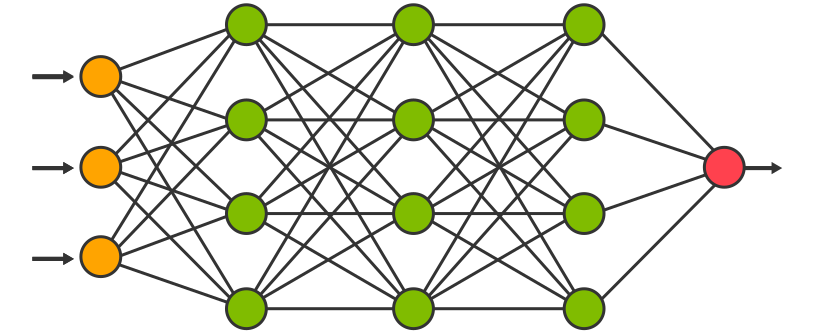
\includegraphics[scale=.3]{Figs/intro.png}}

%%%%%%%%%%%%%%%%%%%%%%%%%%%%%%%%%%%%%%%%%%%%%%%%%%%%%%%%%%%%%%%%%%%%%%%%%%%%%%%%%%%%%%%%%%
%%%%%%%%%%%%%%%%%%%%%%%%%%%%%% Begin Your Document %%%%%%%%%%%%%%%%%%%%%%%%%%%%%%%%%%%%%%%
%%%%%%%%%%%%%%%%%%%%%%%%%%%%%%%%%%%%%%%%%%%%%%%%%%%%%%%%%%%%%%%%%%%%%%%%%%%%%%%%%%%%%%%%%%
\begin{document}
	
%%%%%%%%%%%%%%%%%%%%%%%%%%%%%%%%%%%%%%%%%%%%%%%%%%%%%%%%%%%%%%%%%%%%%%%%%%%%%%%%%%%%%%%%%%
\fontsize{9}{9}
\begin{frame}[noframenumbering, plain]
	\titlepage
\end{frame}

%%%%%%%%%%%%%%%%%%%%%%%%%%%%%%%%%%%%%%%%%%%%%%%%%%%%%%%%%%%%%%%%%%%%%%%%%%%%%%%%%%%%%%%%%%
%\section{Single Layer Perceptron}
%\import{Sections/}{section1.tex}
%\section{Multi Layer Perceptron}
%\import{Sections/}{section2.tex}
%\section{Stochastic Gradient Descent}
%\import{Sections/}{section3.tex}
%\section{Training MLPs}
%\import{Sections/}{section4_training.tex}
%%%%%%%%%%%%%%%%%%%%%%%%%%%%%%%%%%%%%%%%%%%%%%%%%%%%%%%%%%%%%%%%%%%%%%%%


%%%%%%%%%%%%%%%%%%%%%%%%%%[Single Layer]%%%%%%%%%%%%%%%%%%%%%%%%%%%%%%%%%%%%%%%%%%%
\section{Single Layer Perceptron}
\begin{frame}{Biological Analogy}
	\begin{figure}[H]
		\centering
		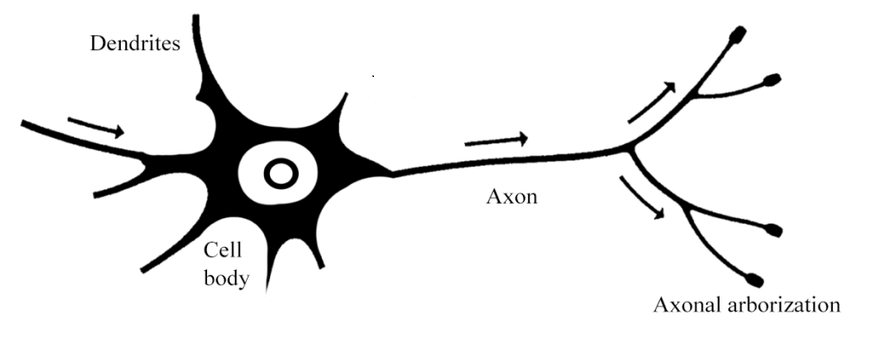
\includegraphics[width=0.9\textwidth]{Figs/biological_neuron.png}
		\caption{Anatomy of a biological neuron \cite{biological-and-nn-neuron}.}
	\end{figure}
\end{frame}

\begin{frame}{Activation Functions}
	\begin{figure}[H]
		\centering
		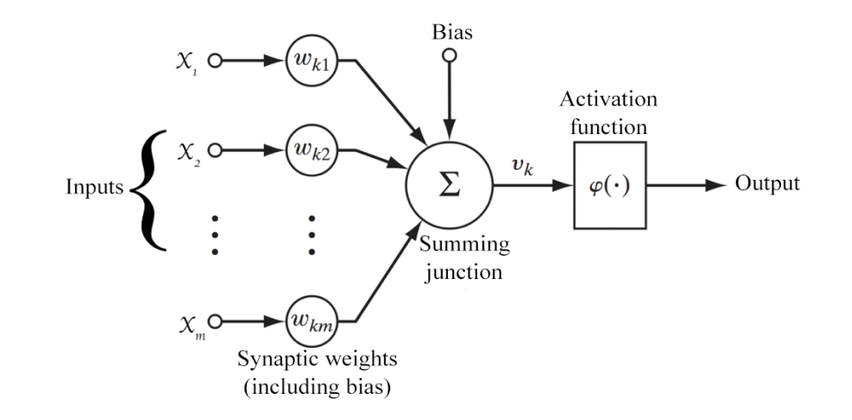
\includegraphics[width=0.9\textwidth]{Figs/nn_neuron.png}
		\caption{Neural network neuron \cite{biological-and-nn-neuron}.}
	\end{figure}
\end{frame}

\begin{frame}{Activation Functions}
	\begin{figure}[H]
		\centering
		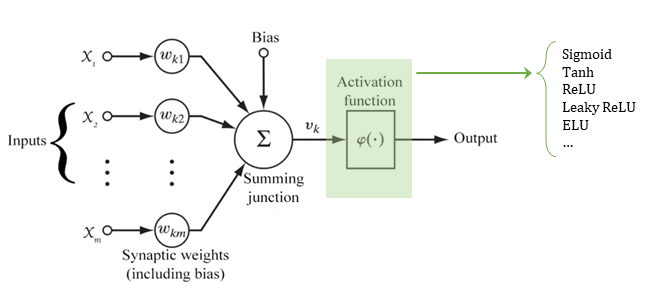
\includegraphics[width=0.9\textwidth]{Figs/activation_function_1.png}
		\caption{Activation function}
	\end{figure}
\end{frame}

\begin{frame}{Activation Functions}
	\begin{figure}[H]
		\centering
		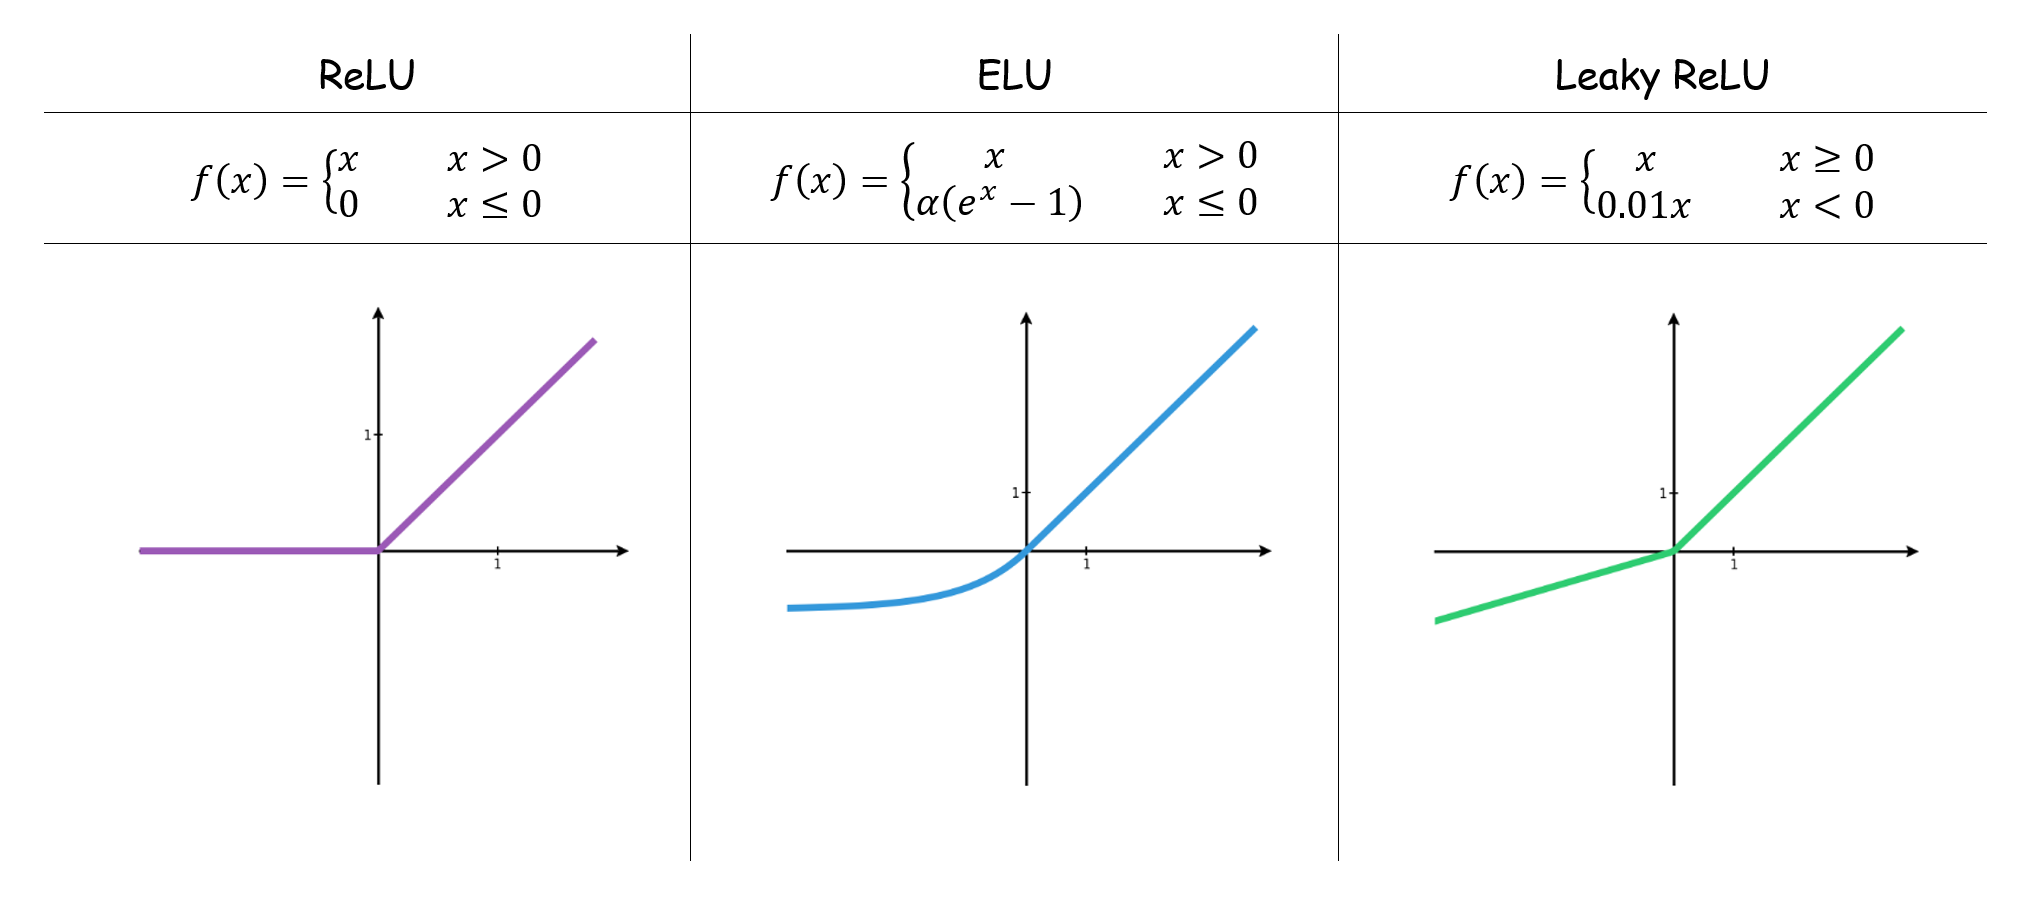
\includegraphics[width=1\textwidth]{Figs/section_1/activation_functions_1.PNG}
	\end{figure}
\end{frame}

\begin{frame}{Activation Functions}
	\begin{figure}[H]
		\centering
		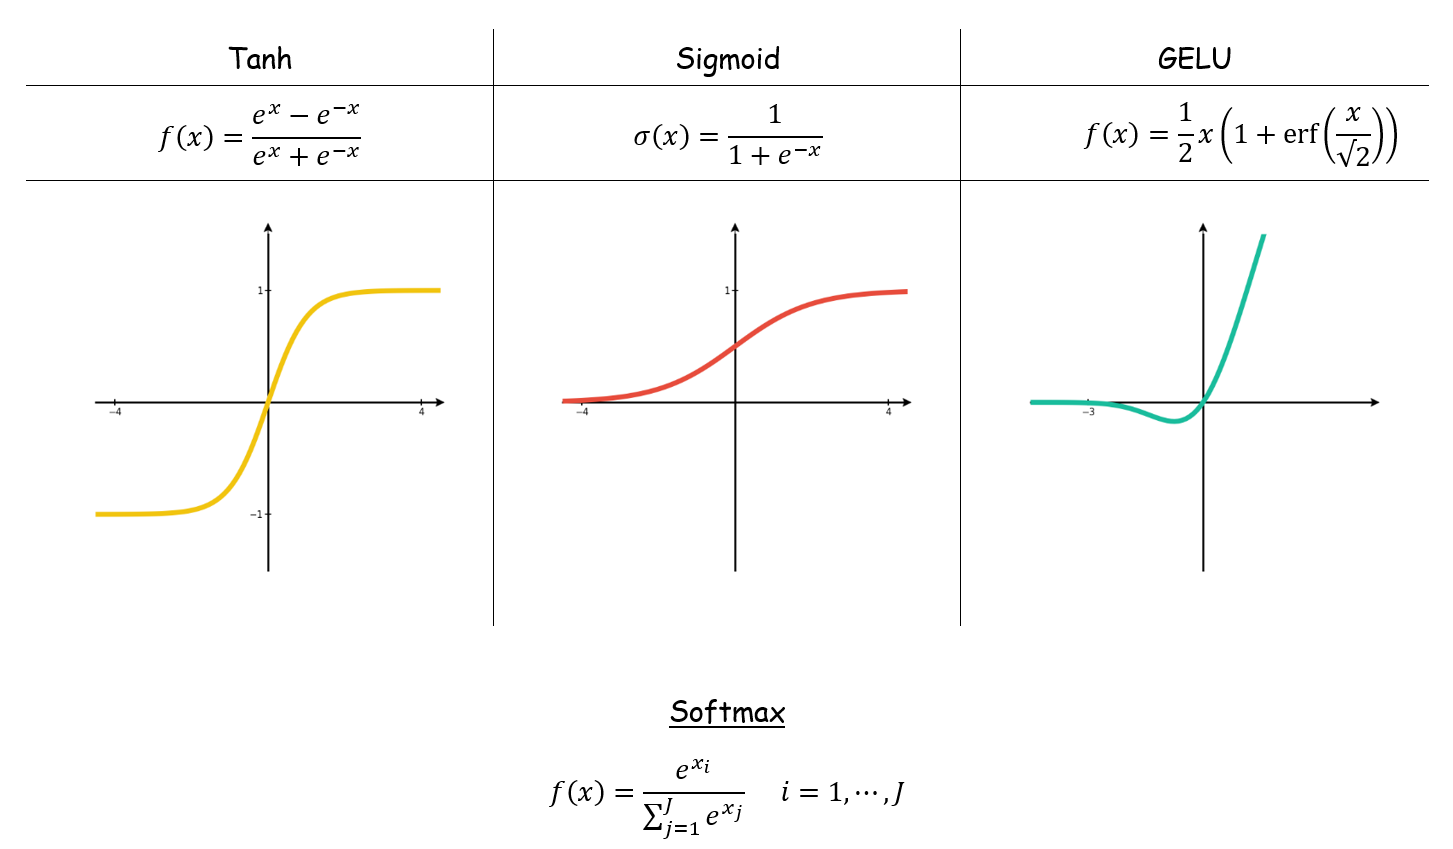
\includegraphics[width=1\textwidth]{Figs/section_1/activation_functions_2.PNG}
	\end{figure}
\end{frame}

\begin{frame}{Gradient Descent}
	\begin{figure}[H]
		\centering
		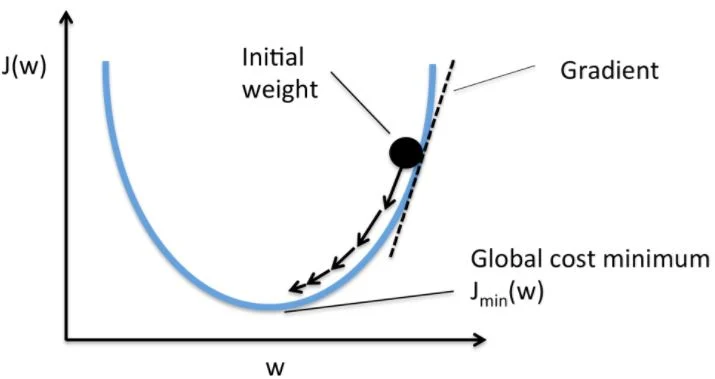
\includegraphics[width=0.70\textwidth]{Figs/gradient_descent2.png}
		\caption{Gradient descent \cite{gradient-descend2}.}
	\end{figure}
\end{frame}

\begin{frame}{Gradient Descent}
	\begin{itemize}
		\item Let's define our problem:
		\begin{itemize}
			\item We have dataset $\mathcal{D} = \{x^{i}, y^{(i)}\}_{i=1}^{n}$.
			\medskip
			\item $f$ is a single layer perceptron.
			\medskip
			\item Define $\hat{y}^{(i)} = f(x^{(i)})$.
		\end{itemize}
		\medskip
		\item We want to minimize following cost function:
		$$
		\mathcal{J}(\bm{w})  = \frac{1}{2} \sum_{i=1}^{n} (y^{(i)} - \hat{y}^{(i)})^2
		$$
		\medskip
		\item We are going to use gradient descent algorithm. $\bm{w}$ will be updated as follows:
		\[
		\bm{w}^{t+1} = \bm{w}^{t} - \eta \nabla_{\bm{w}} \mathcal{J}
		\]
	\end{itemize}
\end{frame}

\begin{frame}{Gradient Descent}
	\begin{itemize}
		\item Let's find $\nabla_{\bm{w}} \mathcal{J}$:
	\end{itemize}
	\vspace*{0.5em}
	\begin{equation*} 
		\begin{split}
			\frac{\partial J}{\partial w_j} & = \frac{\partial }{\partial w_j} \frac{1}{2} \sum_i  (y^{(i)} - \hat{y}^{(i)})^2 \\
			& = \frac{1}{2} \sum_i \frac{\partial}{\partial w_j} (y^{(i)} - \hat{y}^{(i)})^2 \\
			& = \frac{1}{2} \sum_i 2 (y^{(i)} - \hat{y}^{(i)}) \frac{\partial}{\partial w_j} (y^{(i)} - \hat{y}^{(i)}) \\ 
			& = \sum_i (y^{(i)} - \hat{y}^{(i)}) \frac{\partial}{\partial w_j} \bigg(y^{(i)} - \sum_j w_j x^{(i)}_{j}\bigg) \\
			& = \sum_i  (y^{(i)} - \hat{y}^{(i)})(-x^{(i)}_{j}) 
		\end{split}
	\end{equation*}
	
	$$\Delta w_j = - \eta \frac{\partial J}{\partial w_j} = - \eta \sum_i  (y^{(i)} - \hat{y}^{(i)})(- x^{(i)}_{j}) = \eta \sum_i (y^{(i)} - \hat{y}^{(i)})x^{(i)}_{j}$$
	
	$$\mathbf{w} := \mathbf{w} + \Delta \mathbf{w}$$
\end{frame}



%%%%%%%%%%%%%%%%%%%%%%%%%%[Multi Layer Perceptron]%%%%%%%%%%%%%%%%%%%%%%%%%%%%%%%%%%%%%%%%%%%
\section{Multi Layer Perceptron}
\begin{frame}{Limitations of SLP}
	\begin{itemize}
		\item What are the limitations of SLP?
		\item Can we learn all functions with SLP?
	\end{itemize}
	\begin{figure}[H]
		\centering
		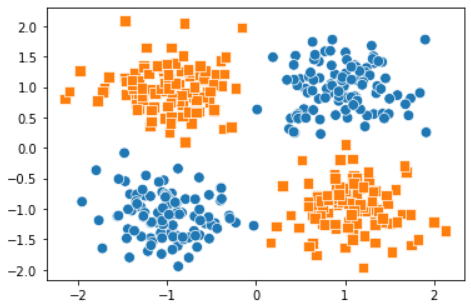
\includegraphics[width=0.6\textwidth]{Figs/xor.png}
		\caption{The XOR function is not linear separable.}
	\end{figure}
\end{frame}

\begin{frame}{Limitations of SLP}
	\begin{itemize}
		\item As we saw in the XOR case, nonlinear separable functions can not be learned by SPLs.
	\end{itemize}
	\begin{figure}[H]
		\centering
		\begin{subfigure}[b]{0.4\textwidth}
			\centering
			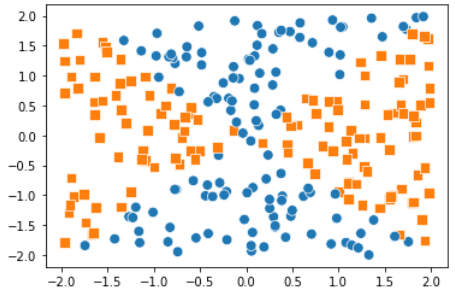
\includegraphics[width=\textwidth]{Figs/non-linear1.png}
		\end{subfigure}
		\hspace*{1.5em}
		\begin{subfigure}[b]{0.4\textwidth}
			\centering
			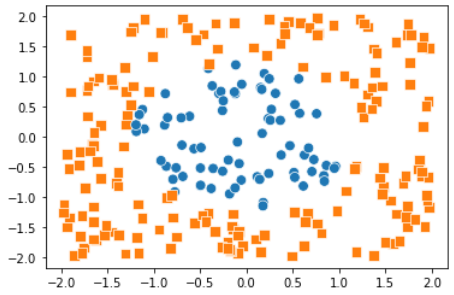
\includegraphics[width=\textwidth]{Figs/non-linear2.png}
		\end{subfigure}
		\caption{Examples of nonlinear separable functions.}
	\end{figure}    
	\begin{itemize}
		\item How to solve this?
	\end{itemize}
\end{frame}

\begin{frame}{Limitations of SLP}
	\begin{itemize}
		\item What if we knew some feature space which our data is linear separable in?!
	\end{itemize}
	\begin{figure}[H]
		\centering
		\begin{subfigure}[b]{0.35\textwidth}
			\centering
			$(x, y)$
			$\vcenter{\hbox{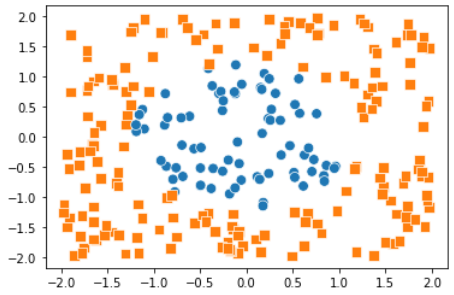
\includegraphics[width=\textwidth]{Figs/non-linear2.png}}}$
		\end{subfigure}
		$\quad\Longrightarrow\quad$
		\begin{subfigure}[b]{0.35\textwidth}
			\centering
			$(r, \theta)$
			$\vcenter{\hbox{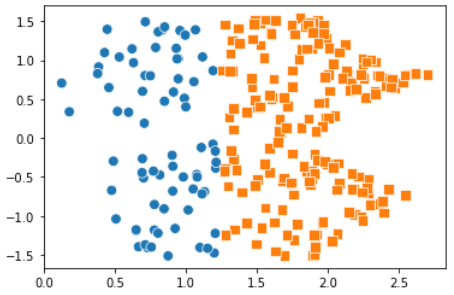
\includegraphics[width=\textwidth]{Figs/circ-linear.png}}}$
		\end{subfigure}
		\caption{Data is linear separable after transformation.}
	\end{figure}
\end{frame}

\begin{frame}{Multi-Layer Perceptron}
	\begin{itemize}
		\item So if we know some $f_1, \cdots, f_4$ we can use SLP to solve problem.
	\end{itemize}
	\begin{figure}[H]
		\centering
		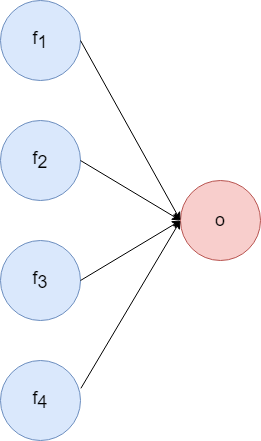
\includegraphics[height=0.45\textheight]{Figs/feature_space.png}
		\caption{Using feature space $f$ to solve problem.}
	\end{figure}
	\begin{itemize}
		\item How to learn this $f_i$s? Use SLP!
	\end{itemize}
\end{frame}

\begin{frame}{Multi-Layer Perceptron}
	\begin{itemize}
		\item We can use inputs ($x_i$) to learn features ($f_i$)
	\end{itemize}
	\begin{figure}[H]
		\centering
		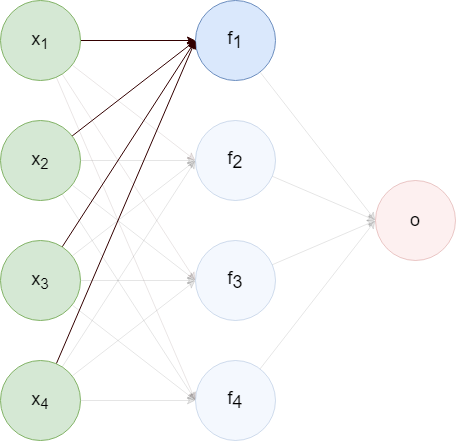
\includegraphics[height=0.45\textheight]{Figs/learn_features.png}
		\caption{Using inputs to learn features.}
	\end{figure}
	\begin{itemize}
		\item What if $f_i$s are not sufficient? We can add more layers!
	\end{itemize}
\end{frame}

\begin{frame}{Multi-Layer Perceptron}
	\begin{itemize}
		\item Adding more layers we will have a bigger network.
	\end{itemize}
	\begin{figure}[H]
		\centering
		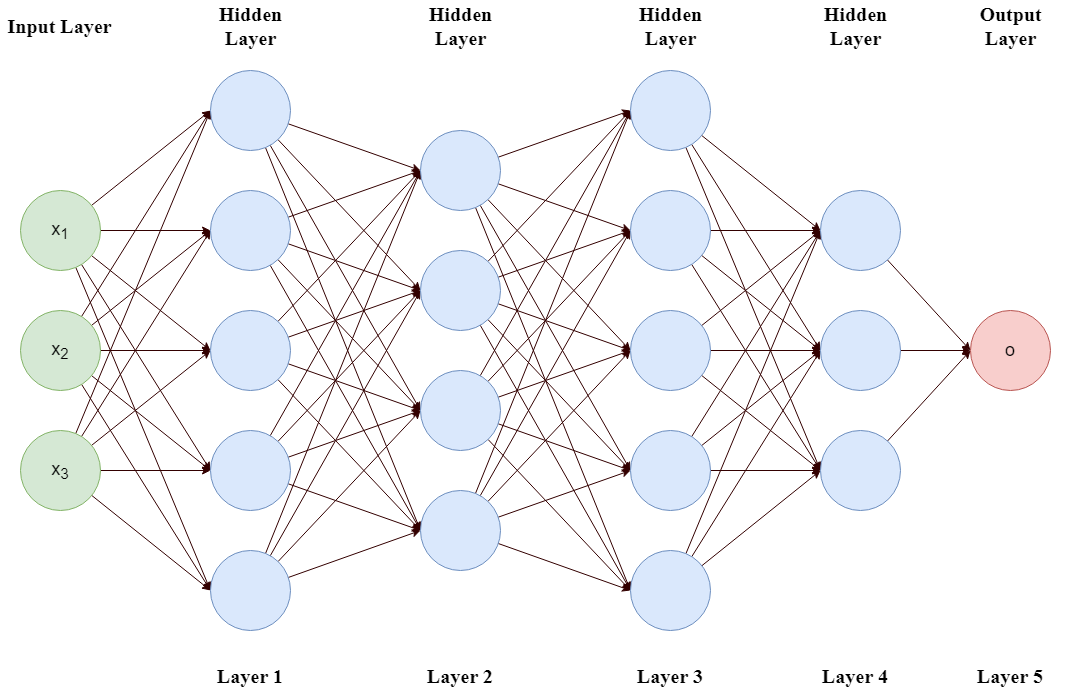
\includegraphics[width=0.8\textwidth]{Figs/5layer_mlp.png}
		\caption{A 5 layer MLP.}
	\end{figure}
\end{frame}


\begin{frame}{Architecture of MLPs}
	\begin{itemize}
		\item Important questions:
		\begin{itemize}
			\item How many hidden layers should we have?
			\item In each hidden layer, how many neurons should we have?
		\end{itemize}
	\end{itemize}
	\begin{figure}[H]
		\centering
		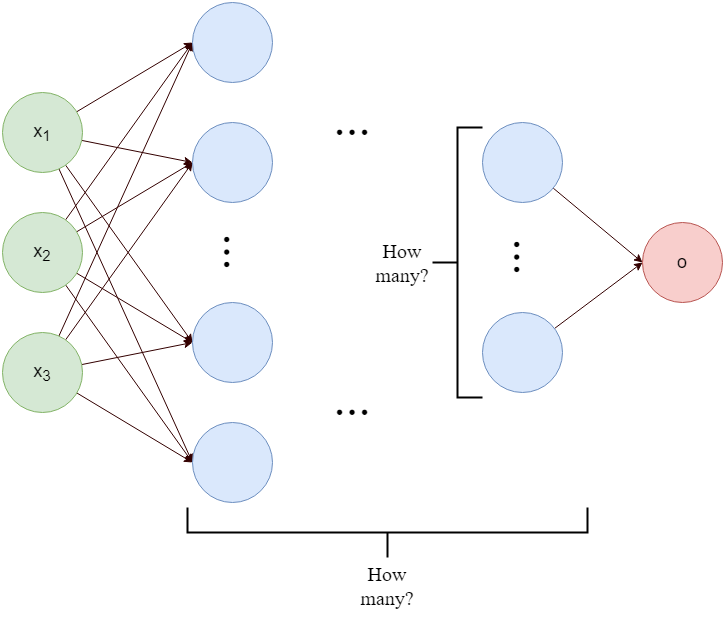
\includegraphics[height=0.6\textheight]{Figs/how_many_layer.png}
		\caption{How many layers and neurons should we have?}
	\end{figure}
\end{frame}


\begin{frame}{Architecture of MLPs}
	\begin{itemize}
		\item In practice:
		\begin{itemize}
			\item You have limited resources
			\item There is no universal rule to choose this hyperparameters
			\item Need to experiment for different number of layers and neurons in each layer
		\end{itemize}
	\end{itemize}
	\begin{figure}[H]
		\centering
		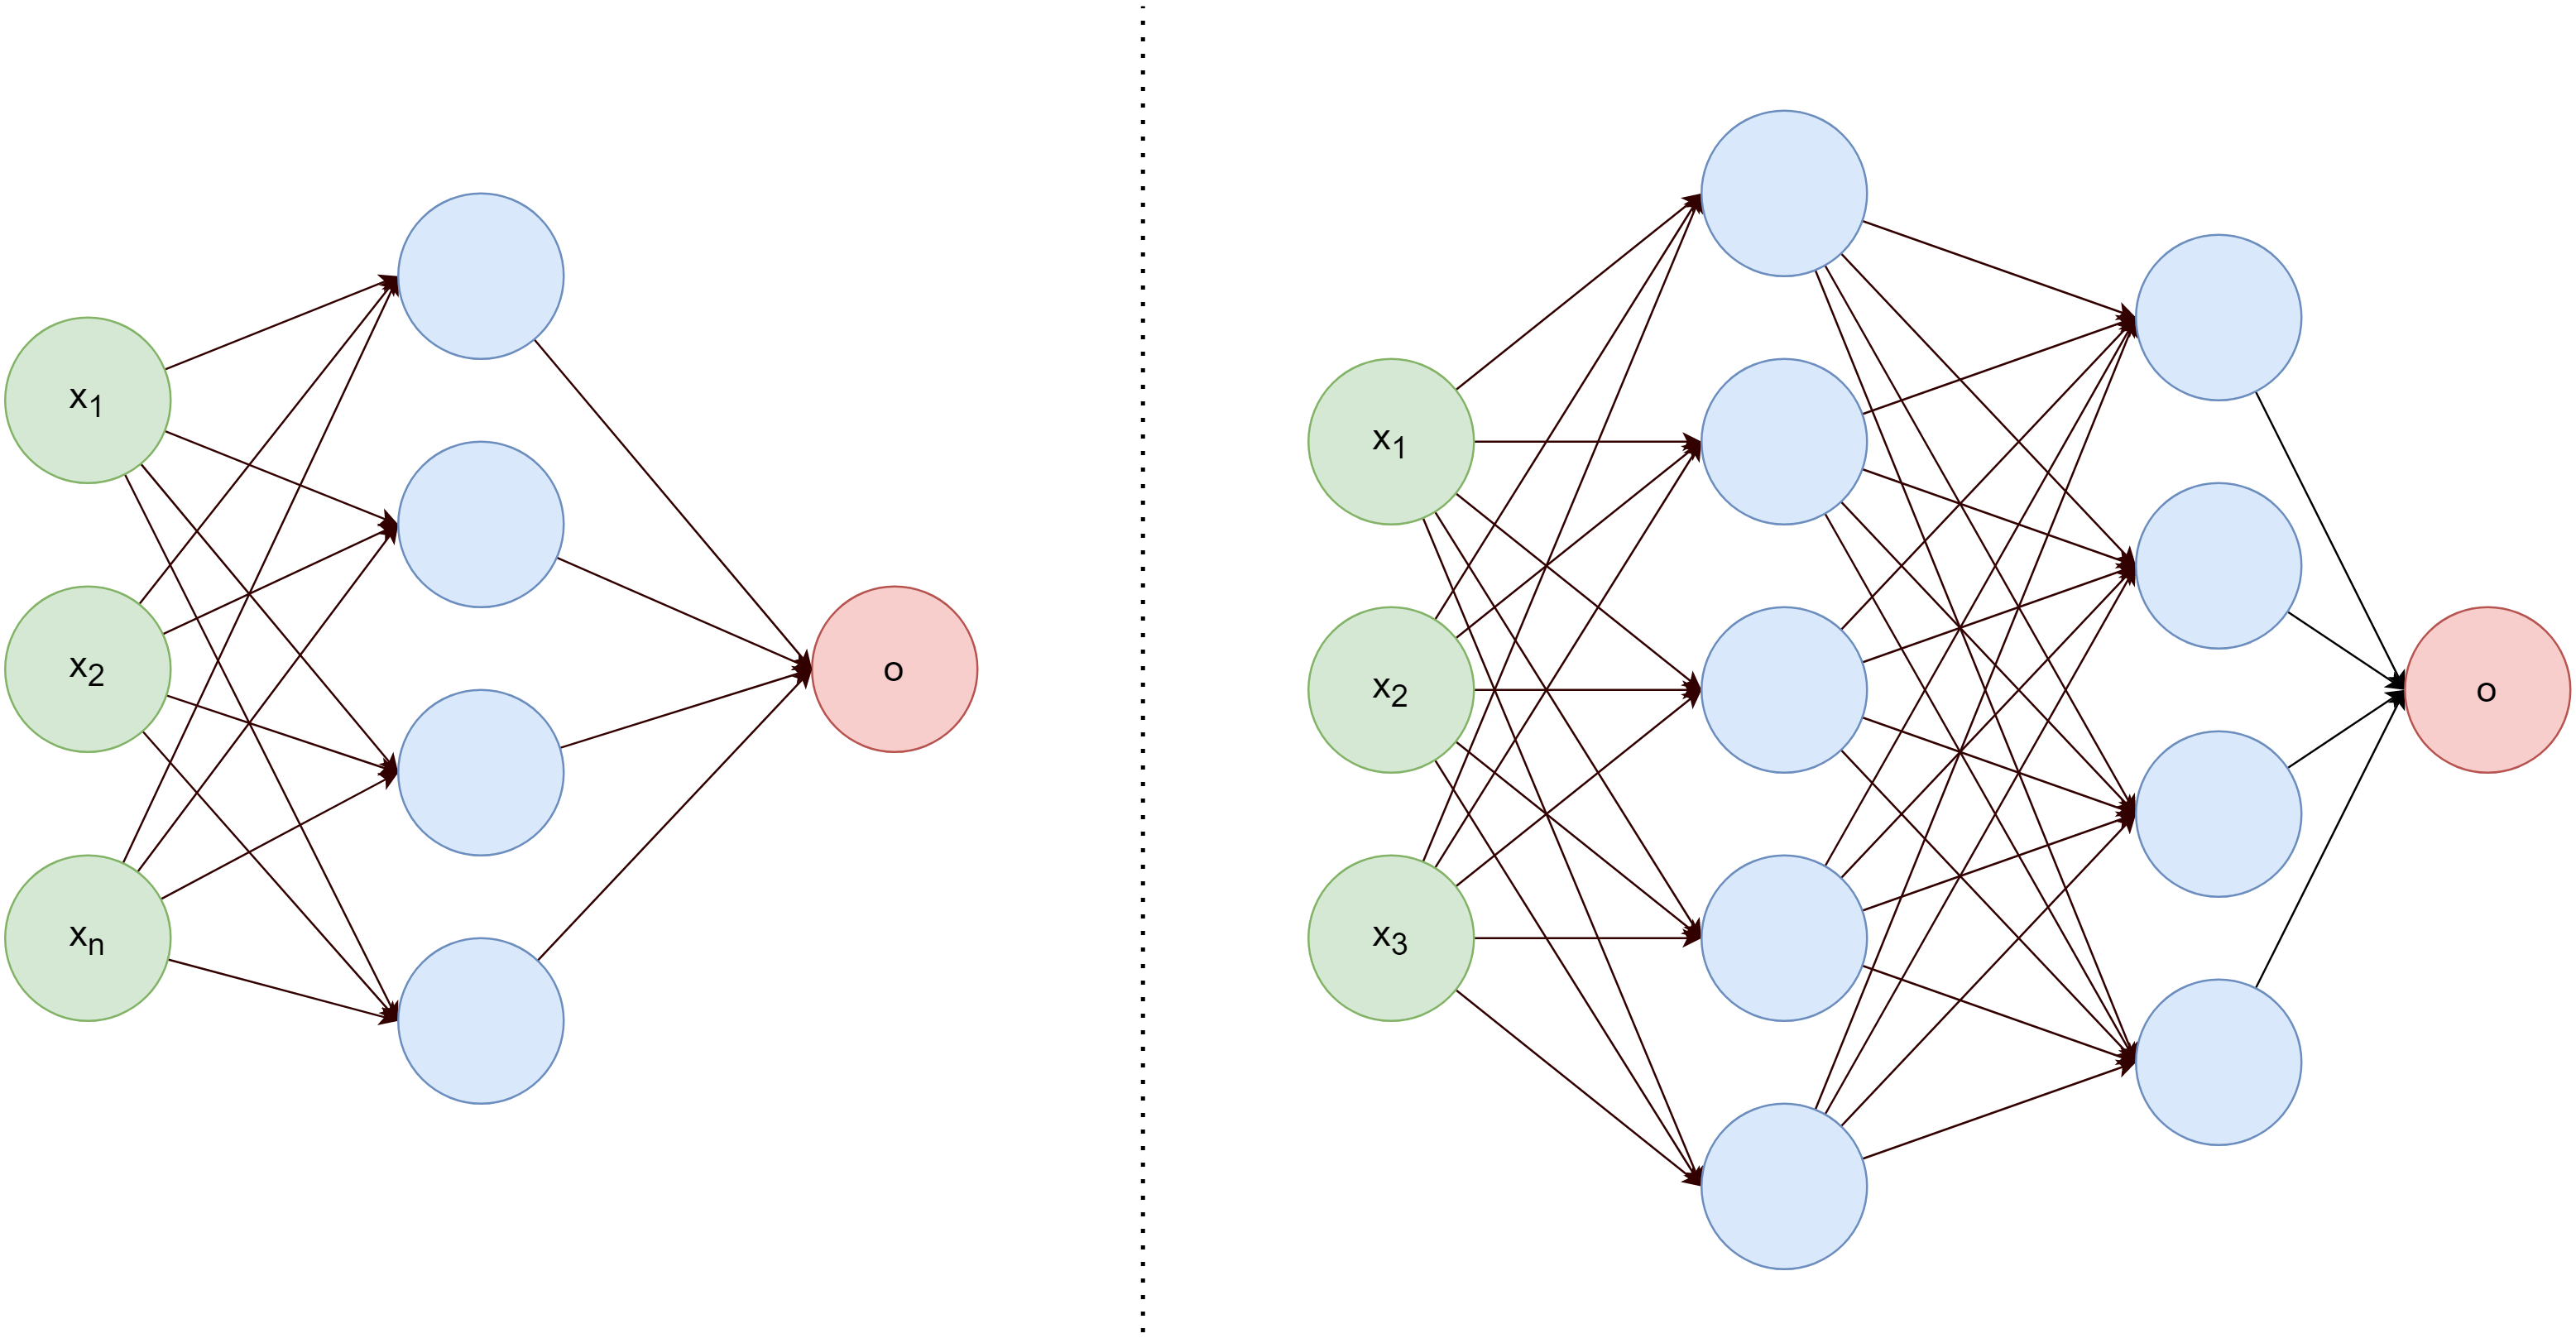
\includegraphics[width=0.6\textwidth]{Figs/experiment_arch.png}
		\caption{Experiment for different architecture and choose the best model.}
	\end{figure}
\end{frame}

\begin{frame}{Activation Function of Hidden Layers}
	\begin{itemize}
		\item One can use any activation function for each hidden units
		\item Usually people use the same activation function for all neurons in one layer
		\item The important point is to use \tc{keywords}{nonlinear} activation functions
	\end{itemize}
	\begin{figure}[H]
		\centering
		\begin{subfigure}[b]{0.55\textwidth}
			\centering
			$\vcenter{\hbox{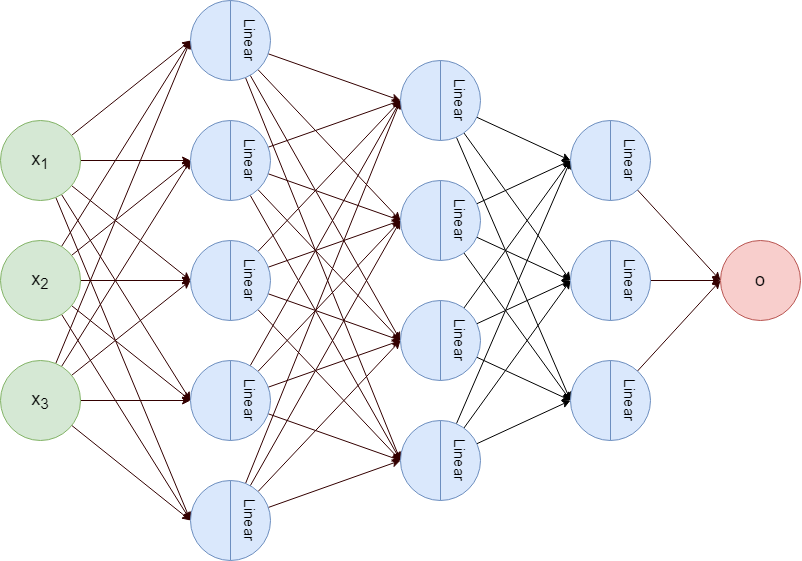
\includegraphics[width=\textwidth]{Figs/linear_neurons.png}}}$
		\end{subfigure}
		$\quad\equiv\quad$
		\begin{subfigure}[b]{0.15\textwidth}
			\centering
			$\vcenter{\hbox{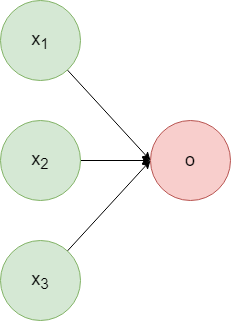
\includegraphics[width=\textwidth]{Figs/simple_slp.png}}}$
		\end{subfigure}
		\caption{MLP with linear activation functions is equivalent to simple SLP.}
	\end{figure}
\end{frame}

\begin{frame}{XOR problem}
	\begin{itemize}
		\item Now let's solve XOR problem with MLPs.
		\item We have two binary inputs, build an MLP to calculate their \textbf{XOR}.
		\medskip
		\medskip
		\item First let's build logical \textbf{AND} and \textbf{OR} functions.
	\end{itemize}
	\begin{figure}[H]
		\centering
		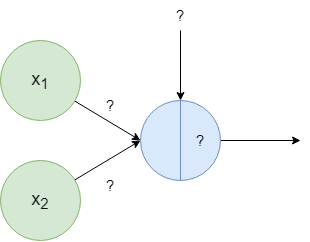
\includegraphics[width=0.35\textwidth]{Figs/solve_and_or_gate.png}
		\caption{We need to find weights, biases and activation function.}
	\end{figure}
\end{frame}

\begin{frame}{XOR problem}
	\begin{figure}
		\centering
		\begin{subfigure}[b]{0.25\textwidth}
			\centering
			$\vcenter{\hbox{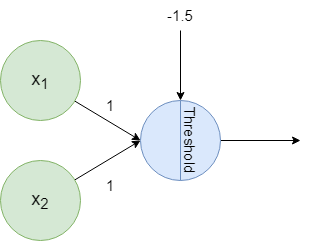
\includegraphics[width=\textwidth]{Figs/and_gate.png}}}$
			\caption{$x_1 \wedge x_2$}
		\end{subfigure}
		\hspace*{0.5em}
		\begin{subfigure}[b]{0.25\textwidth}
			\centering
			$\vcenter{\hbox{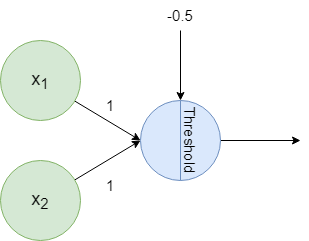
\includegraphics[width=\textwidth]{Figs/or_gate.png}}}$
			\caption{$x_1 \vee x_2$}
		\end{subfigure}
		\hspace*{0.5em}
		\begin{subfigure}[b]{0.25\textwidth}
			\centering
			$\vcenter{\hbox{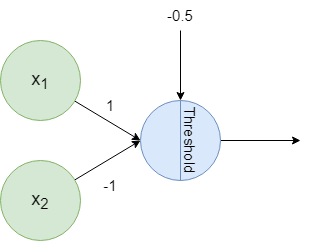
\includegraphics[width=\textwidth]{Figs/and_not_gate.png}}}$
			\caption{$x_1 \wedge \overline{x_2}$}
		\end{subfigure}
	\end{figure}
	\pause
	\begin{figure}[H]
		\centering
		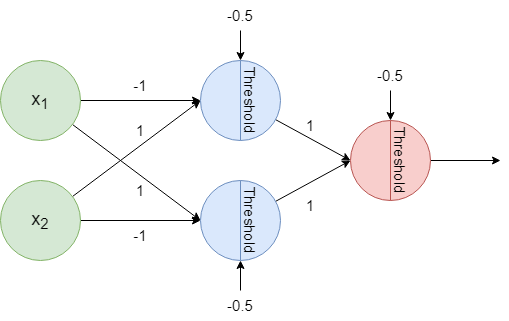
\includegraphics[height=0.35\textheight]{Figs/xor_gate.png}
		\caption{MLP for XOR function.}
	\end{figure}
\end{frame}


% \begin{frame}{Example of universality}
	%     \begin{itemize}
		%         \item ToDo
		%     \end{itemize}
	% \end{frame}


\begin{frame}{MLP notation}
	\begin{itemize}
		\item $a^{[l]}_i$: $i$-th neuron output in layer $l$
		\item $\bm{a}^{[l]}$: layer $l$ output in vector form
	\end{itemize}
	\begin{figure}[H]
		\centering
		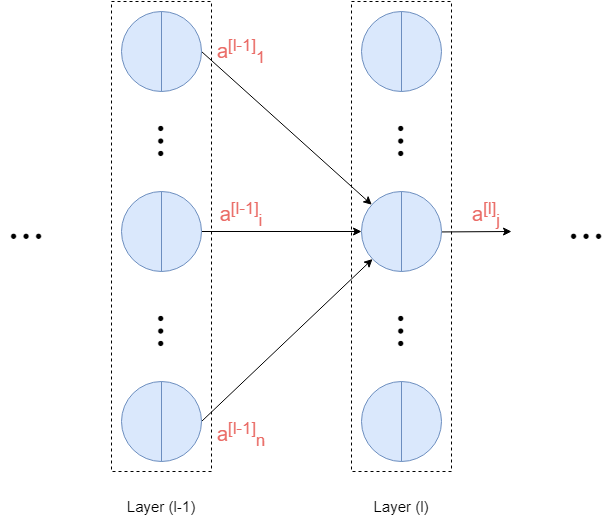
\includegraphics[width=0.5\textwidth]{Figs/notation1.png}
	\end{figure}
\end{frame}

\begin{frame}{MLP notation}
	\begin{itemize}
		\item $b^{[l]}_i$: $i$-th neuron bias in layer $l$
		\item $\bm{b}^{[l]}$: layer $l$ biases in vector form
	\end{itemize}
	\begin{figure}[H]
		\centering
		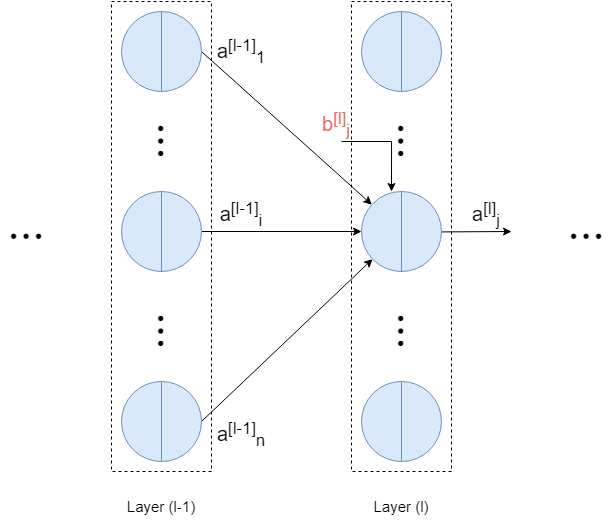
\includegraphics[width=0.5\textwidth]{Figs/notation1.2.png}
	\end{figure}
\end{frame}

\begin{frame}{MLP notation}
	\begin{itemize}
		\item $W^{[l]}_{ij}$: weight of the edge between $i$-th neuron in layer $l-1$ and $j$-th neuron in layer $l$ 
	\end{itemize}
	\begin{figure}[H]
		\centering
		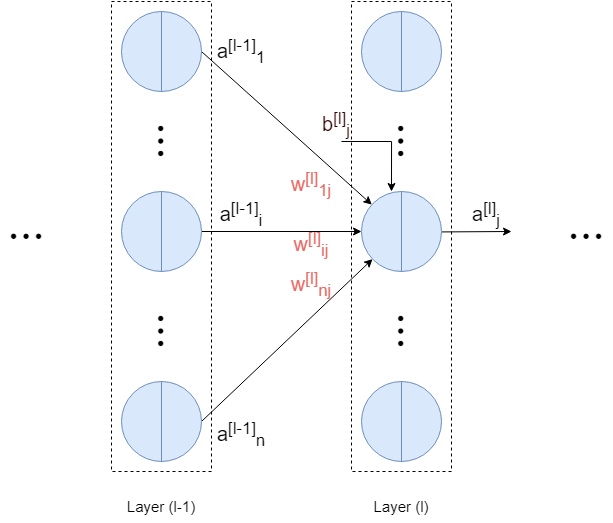
\includegraphics[width=0.5\textwidth]{Figs/notation2.png}
	\end{figure}
\end{frame}

\begin{frame}{MLP notation}
	\begin{itemize}
		\item $z^{[l]}_j$: $j$-th neuron input in layer $l$
		\item $z^{[l]}_j = b_j^{[l]} + \sum_{i=1}^n W^{[l]}_{ij}a^{[l-1]}_i$
	\end{itemize}
	\begin{figure}[H]
		\centering
		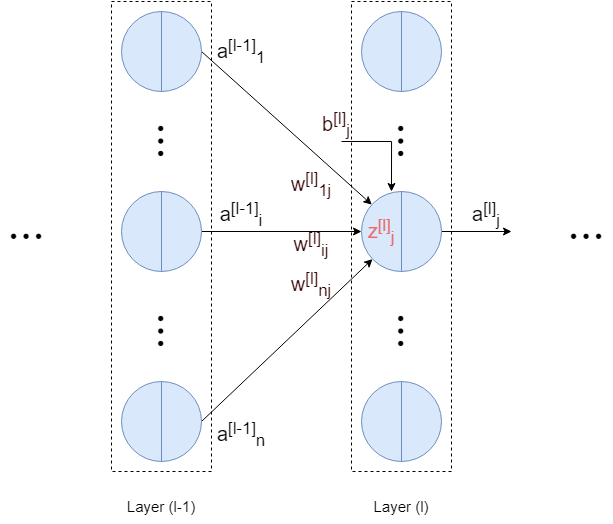
\includegraphics[width=0.5\textwidth]{Figs/notation3.png}
	\end{figure}
\end{frame}

\begin{frame}{MLP notation}
	\begin{itemize}
		\item $\bm{z}^{[l]}$: input of layer $l$ in vector form
		\item $\bm{z}^{[l]} = \bm{b}^{[l]} + (W^{[l]})^T \bm{a}^{[l-1]}$
	\end{itemize}
	\begin{figure}[H]
		\centering
		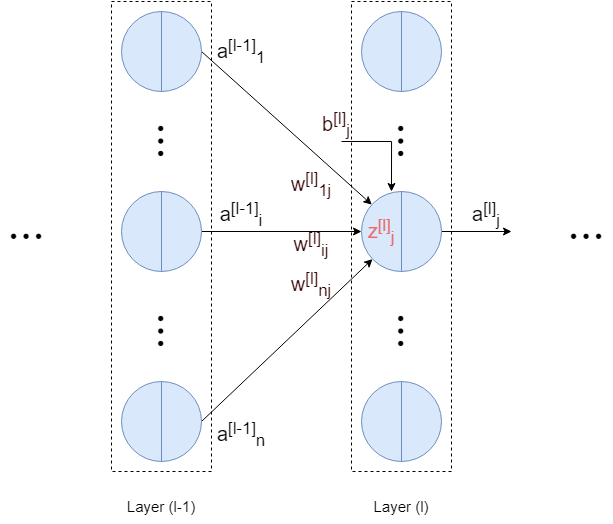
\includegraphics[width=0.5\textwidth]{Figs/notation3.png}
	\end{figure}
\end{frame}

\begin{frame}{MLP notation}
	\begin{itemize}
		\item $\sigma^{[l]}_j$: $j$-th neuron activation function in layer $l$
	\end{itemize}
	\begin{figure}[H]
		\centering
		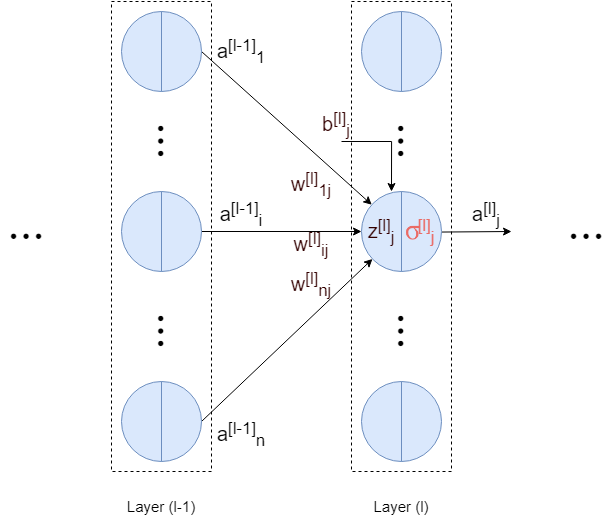
\includegraphics[width=0.5\textwidth]{Figs/notation4.png}
	\end{figure}
\end{frame}

\begin{frame}{MLP notation}
	\begin{itemize}
		\item If we assume all neurons in one layer have the same activation function then:
		\[
		\bm{a}^{[l]} = \sigma^{[l]}\left(\bm{b}^{[l]} +  (W^{[l]})^T\bm{a}^{[l-1]}\right)
		\]
	\end{itemize}
	\begin{figure}[H]
		\centering
		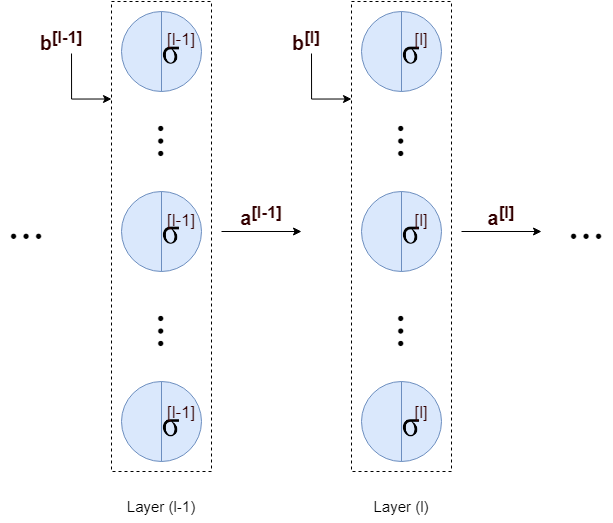
\includegraphics[width=0.5\textwidth]{Figs/notation5.png}
	\end{figure}
\end{frame}

\begin{frame}{MLP notation}
	\begin{itemize}
		\item So for a network with $L$ layer, and $\bm{x}$ as its input we will have:
	\end{itemize}
	\begin{figure}[H]
		\centering
		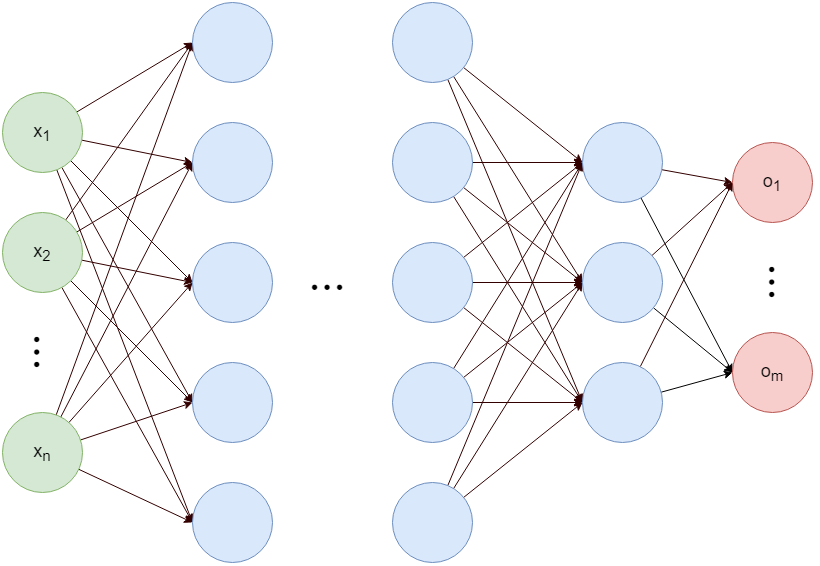
\includegraphics[width=0.6\textwidth]{Figs/notation6.png}
	\end{figure}
	% \[
	% \bm{o}=\bm{a}^{[L]}=\sigma^{[L]}\left((W^{[L]})^T\sigma^{[L-1]}\left((W^{[L-1]})^T\sigma^{[L-2]}\left(\cdots\sigma^{[1]}\left((W^{[1]})^T\bm{x}\right)\cdots \right)\right)\right)
	% \]
	\[
	\bm{o}=\bm{a}^{[L]}=\sigma^{[L]}\left(\bm{b}^{[L]} + (W^{[L]})^T\sigma^{[L-1]}\left(\cdots\sigma^{[1]}\left(\bm{b}^{[1]}+(W^{[1]})^T\bm{x}\right)\cdots \right)\right)
	\]
\end{frame}

\begin{frame}{Learning MLPs}
	\begin{itemize}
		\item Till here we have used networks with predefined weights and biases.
		\item How to learn these parameters?
		\medskip
		\medskip
		\medskip
		\item The idea is to use gradient descent
	\end{itemize}
	\begin{figure}
		\centering
		\begin{subfigure}[b]{0.3\textwidth}
			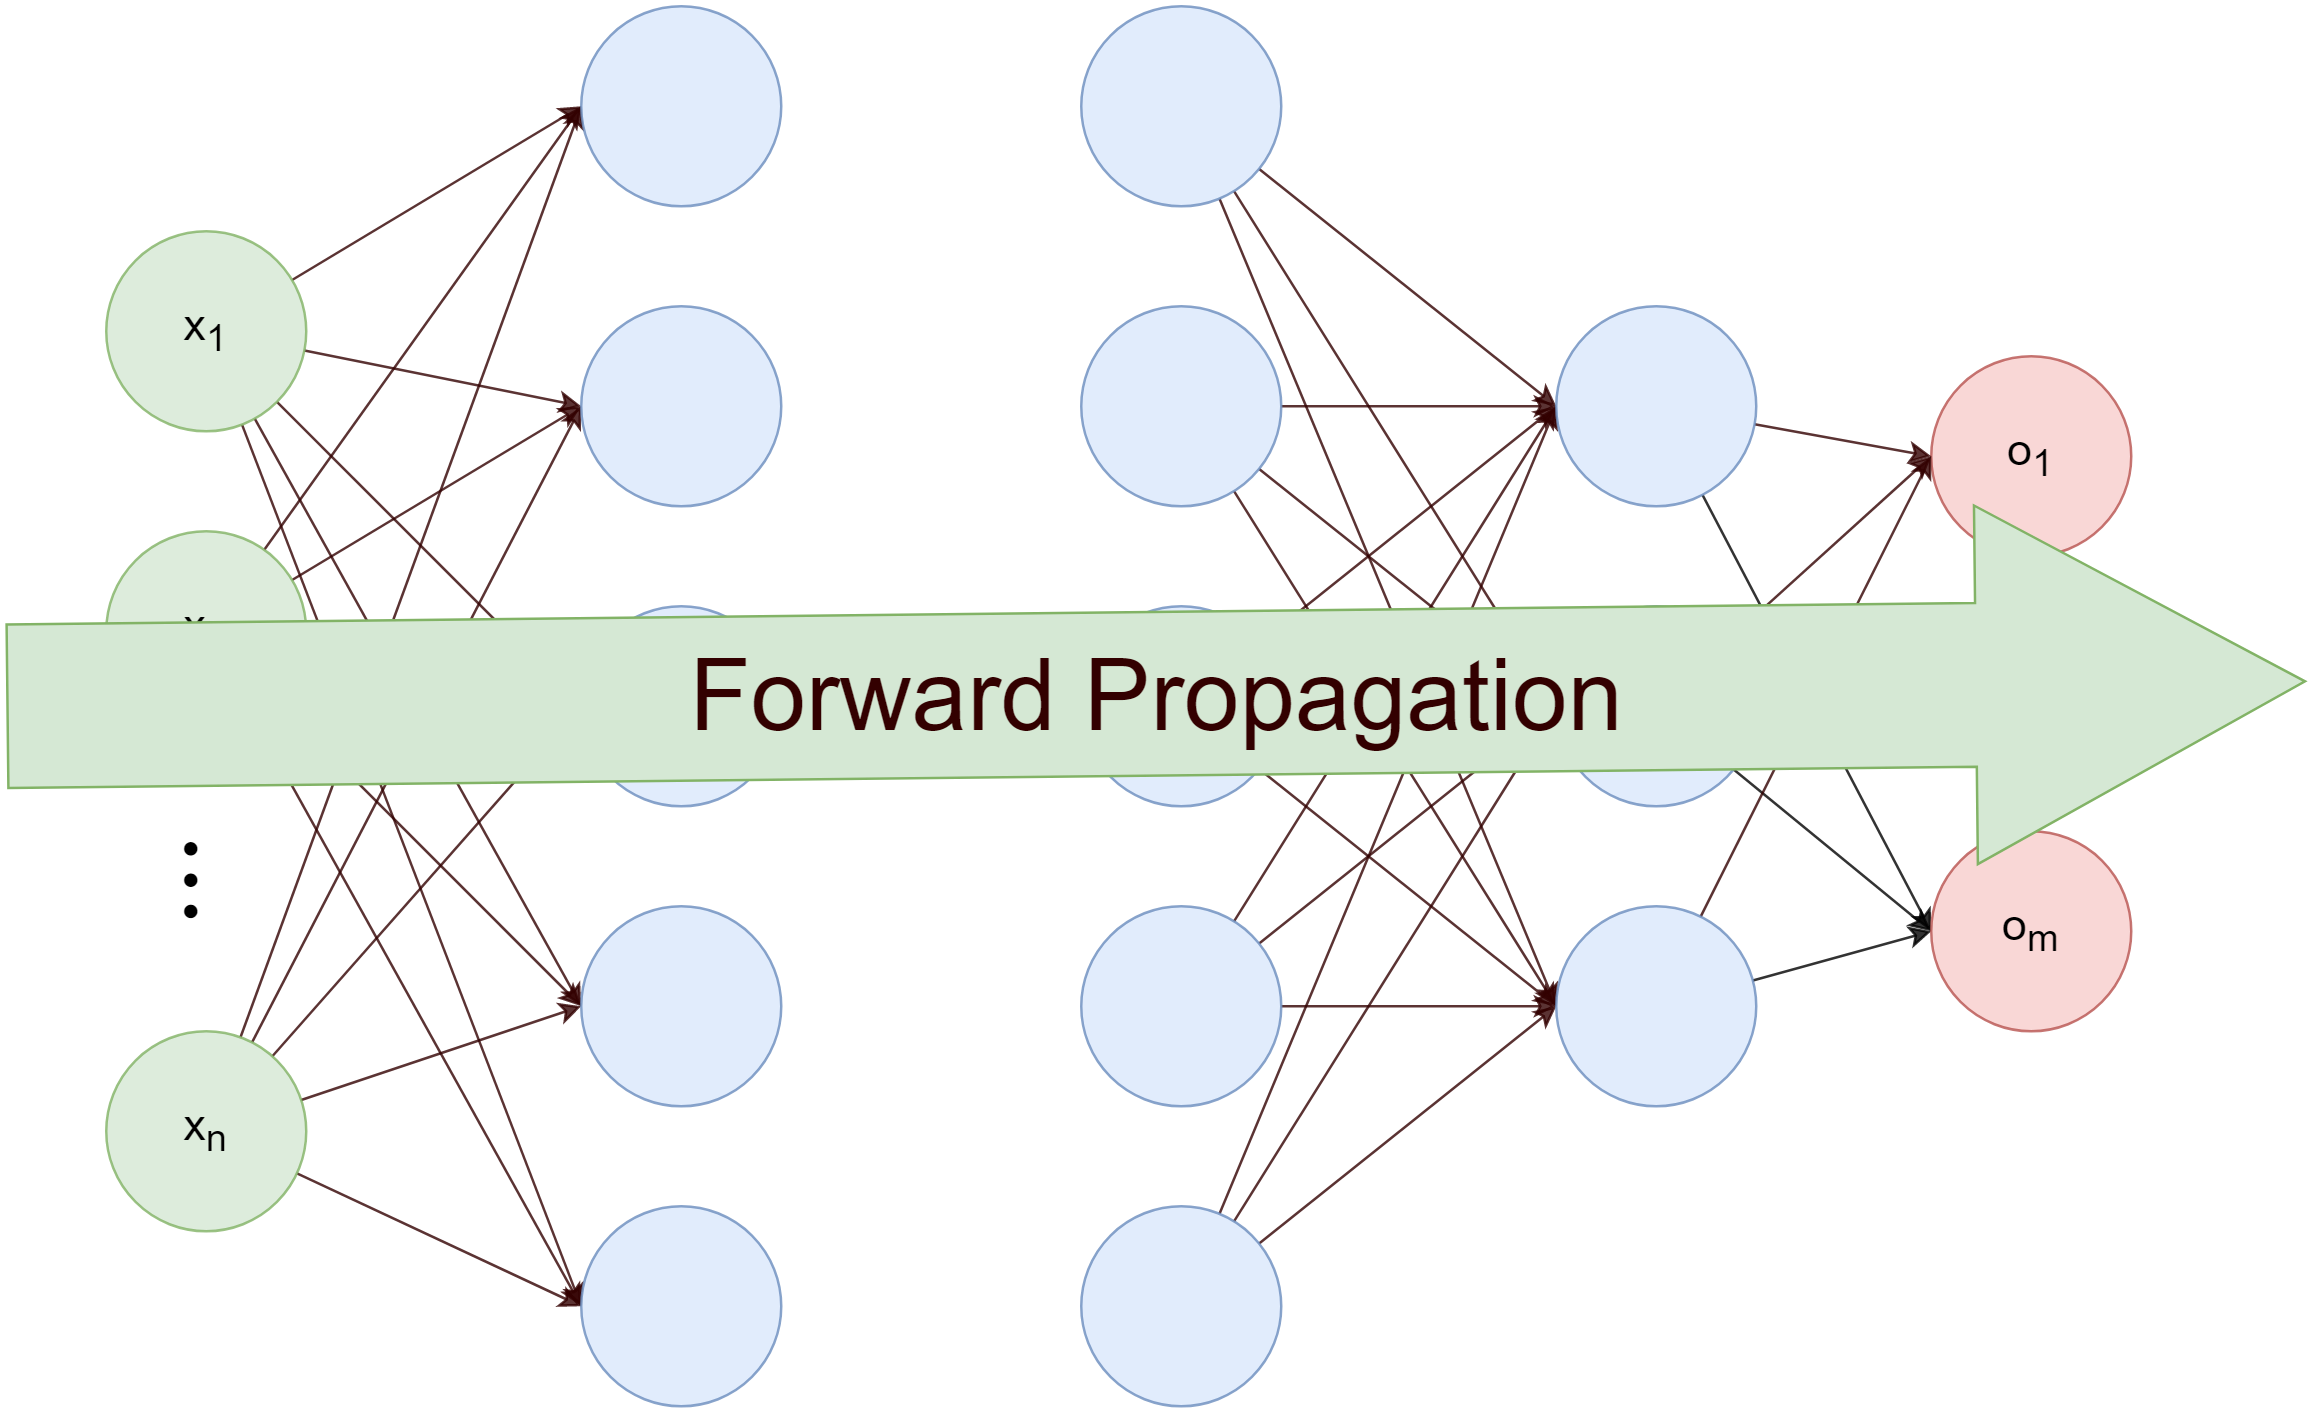
\includegraphics[width=\textwidth]{Figs/forward_propagation.png}
			\caption{Forward pass}
		\end{subfigure}
		\begin{subfigure}[b]{0.3\textwidth}
			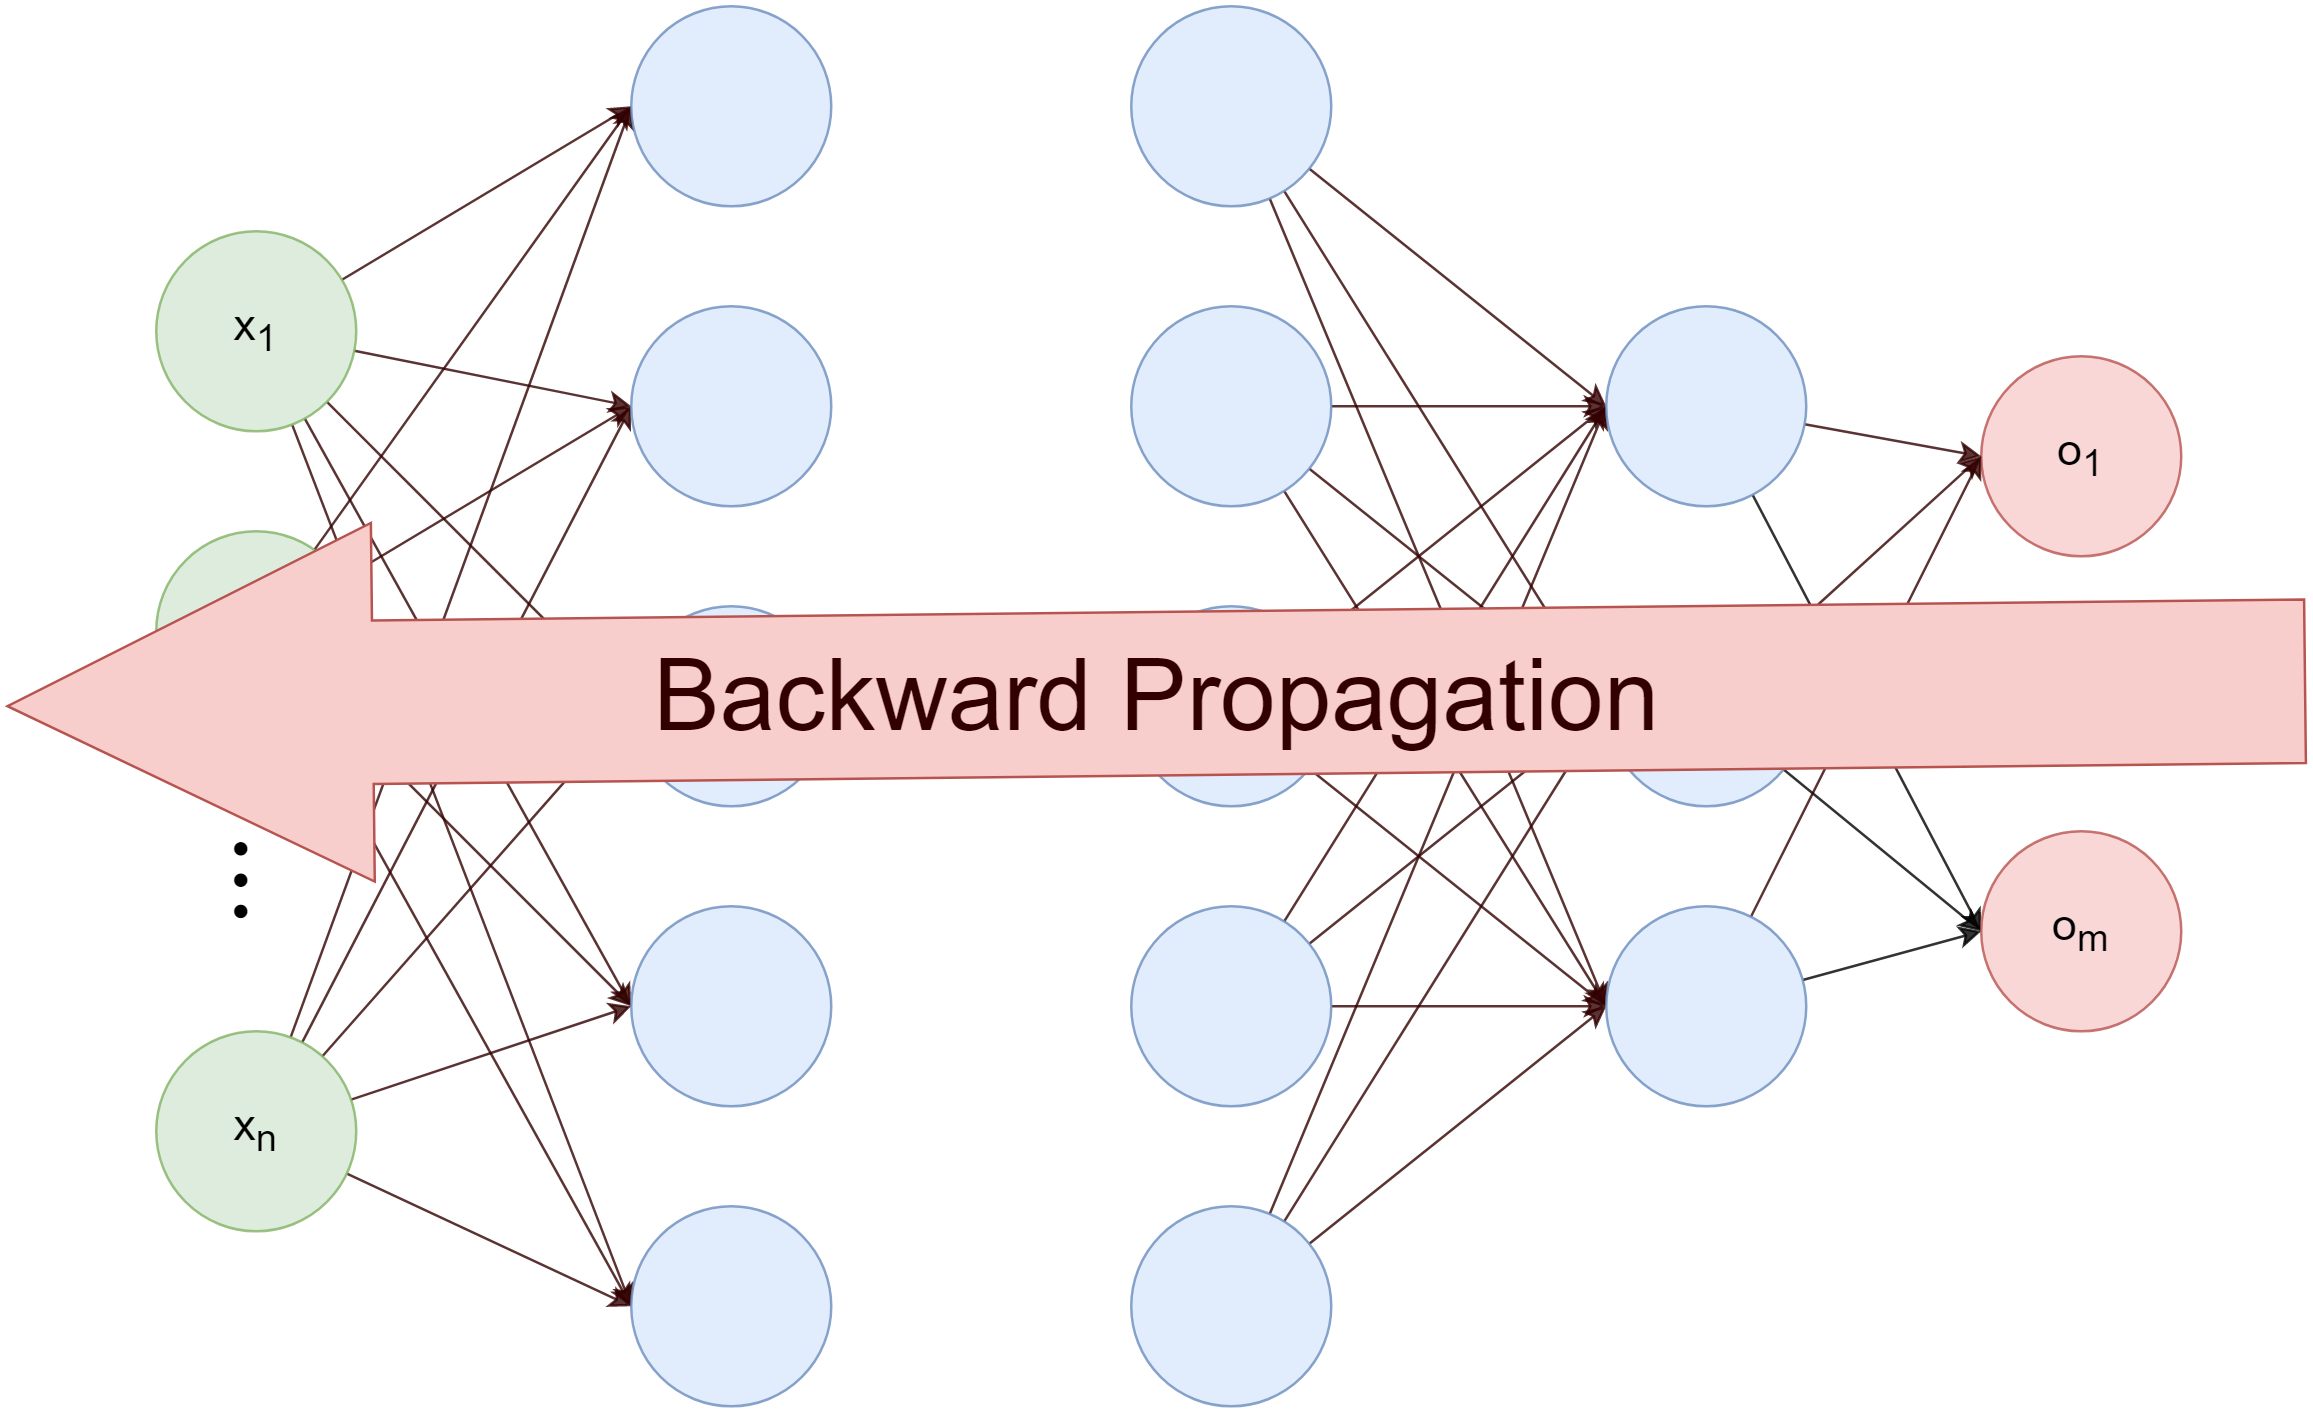
\includegraphics[width=\textwidth]{Figs/backward_propagation.png}
			\caption{Backward pass}
		\end{subfigure}
		\begin{subfigure}[b]{0.28\textwidth}
			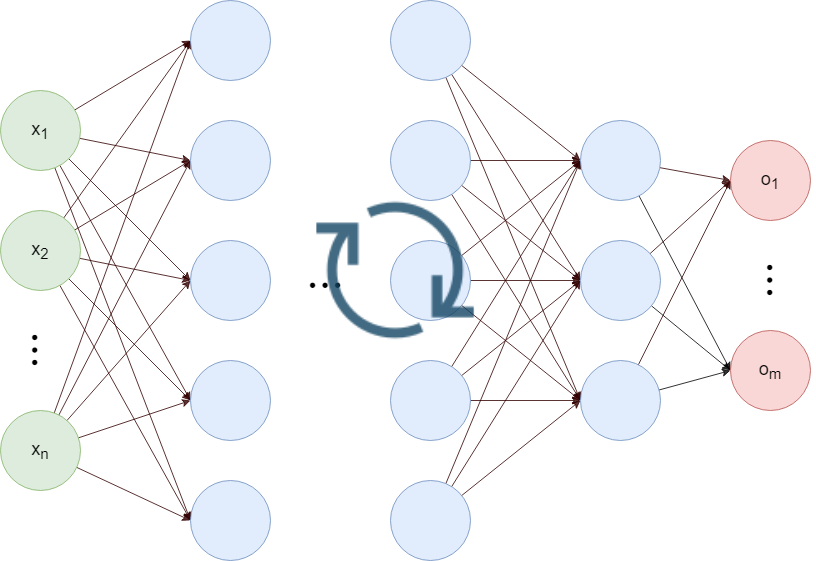
\includegraphics[width=\textwidth]{Figs/update_phase.png}
			\caption{Update parameters}
		\end{subfigure}
	\end{figure}
\end{frame}

\begin{frame}{Learning MLPs}
	\begin{itemize}
		\item Let's define the learning problem more formal:
		\begin{itemize}
			\item $\{(x^{(i)}, y^{(i)})\}_{i=1}^{n}$: dataset
			\item $f$: network
			\item $W$: all weights and biases of the network ($W^{[l]}$ and $\bm{b}^{[l]}$ for different $l$)
			\item $L$: loss function
		\end{itemize}
		\medskip
		\item We want to find $W^{\ast}$ which minimizes following cost function:
		\[
		\mathcal{J}(W) = \sum_{i=1}^{n} L\left(f(x^{(i)}; W), y^{(i)}\right)
		\]
		\item We are going to use gradient descent, so we need to find $\nabla_W \mathcal{J}$.
	\end{itemize}
\end{frame}

\begin{frame}{Forward Propagation}
	\begin{itemize}
		\item First of all we need to find loss value.
		\item It only requires to know the inputs of each neuron.
	\end{itemize}
	\begin{figure}[H]
		\centering
		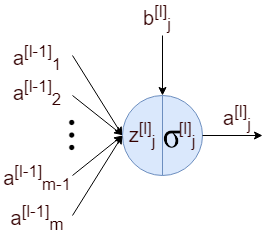
\includegraphics[width=0.3\textwidth]{Figs/forward_pass.png}
		\caption{$a^{[l]}_j = \sum_{i=1}^m W^{[l]}_{ij}a^{[l-1]}_i + b^{[l]}_j$}
	\end{figure}
	\begin{itemize}
		\item So we can calculate these outputs layer by layer.
	\end{itemize}
\end{frame}

\begin{frame}{Forward Propagation}
	\begin{itemize}
		\item After forward pass we will know:
		\begin{itemize}
			\item Loss value
			\item Network output
			\item Middle values
		\end{itemize}
	\end{itemize}
	\begin{figure}[H]
		\centering
		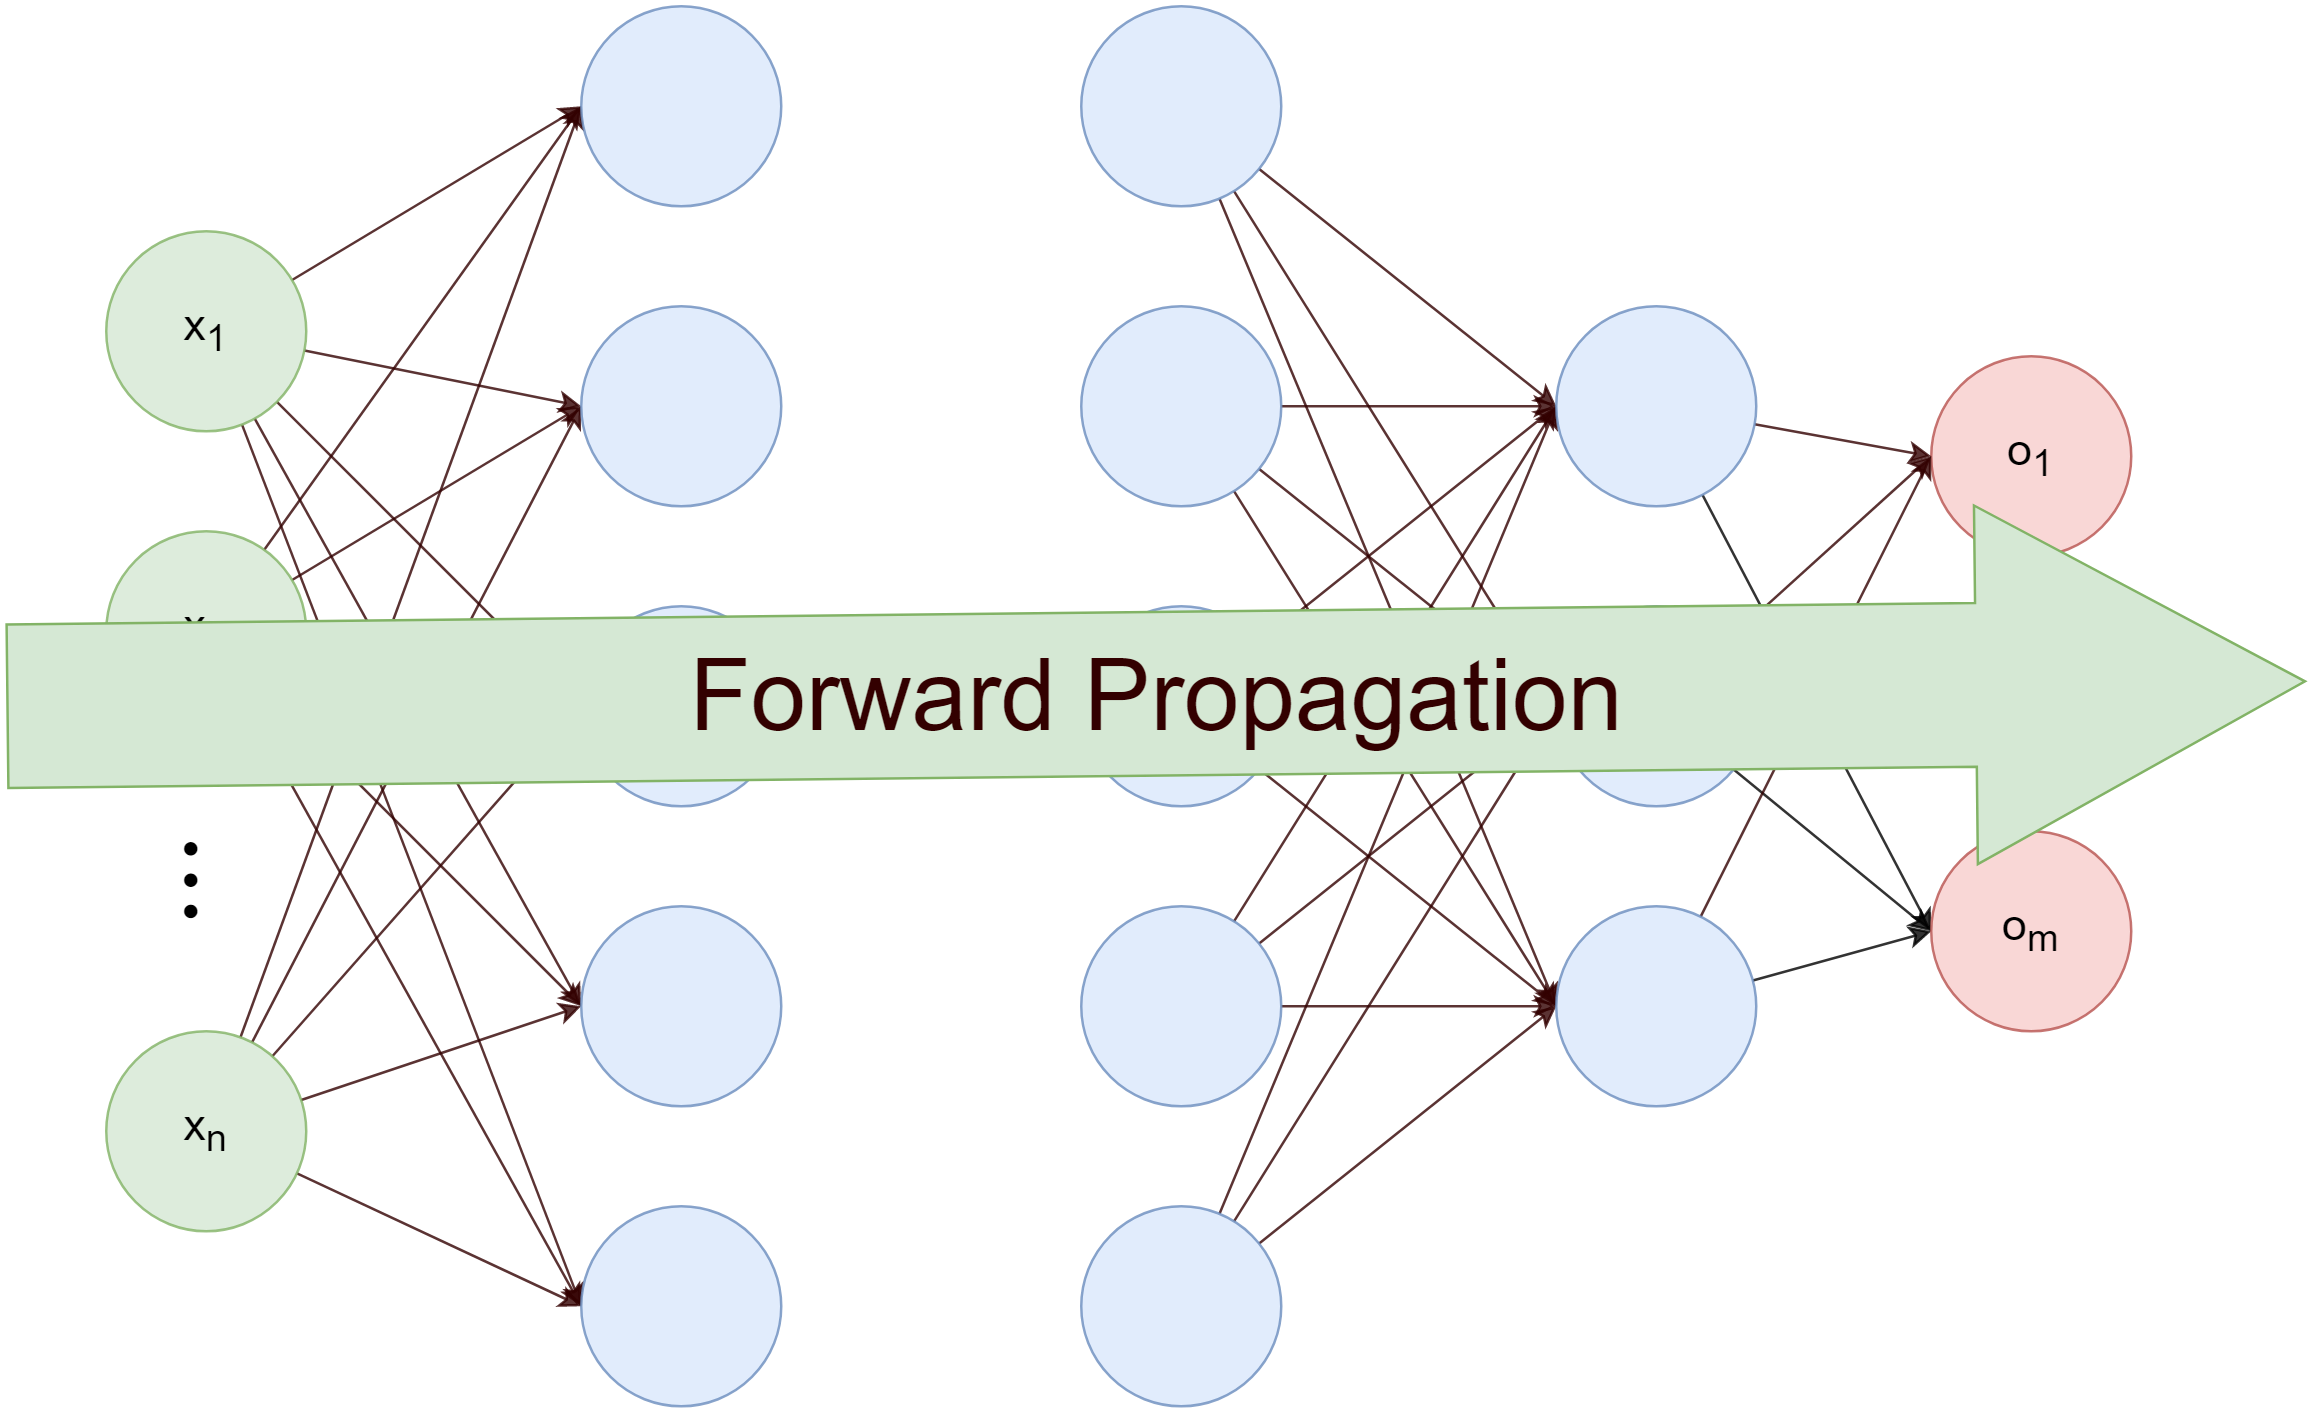
\includegraphics[width=0.5\textwidth]{Figs/forward_propagation.png}
		\caption{Forward pass}
	\end{figure}
\end{frame}

\begin{frame}{Backward Propagation}
	\begin{itemize}
		\item Now we need to calculate $\nabla_W \mathcal{J}$.
		\medskip
		\item First idea:
		\begin{itemize}
			\item Use analytical approach.
			\item Write down derivatives on paper.
			\item Find the close form of $\nabla_W \mathcal{J}$ (if it is possible to do so).
			\item Implement this gradient as a function to work with.
			\medskip
			\medskip
			\item Pros:
			\begin{itemize}
				\item Fast
				\item Exact
			\end{itemize}
			\medskip
			\medskip
			\item Cons:
			\begin{itemize}
				\item Need to rewrite calculation for different architectures
			\end{itemize}
		\end{itemize}
	\end{itemize}
\end{frame}

\begin{frame}{Backward Propagation}
	\begin{itemize}
		\item Second idea:
		\begin{itemize}
			\item Using \tc{keywords}{modular} approach.
			\item Computing the cost function consists of doing many operations.
			\item We can build a computation graph for this calculation.
			\item Each node will represent a single operation.
		\end{itemize}
	\end{itemize}
	\begin{figure}[H]
		\centering
		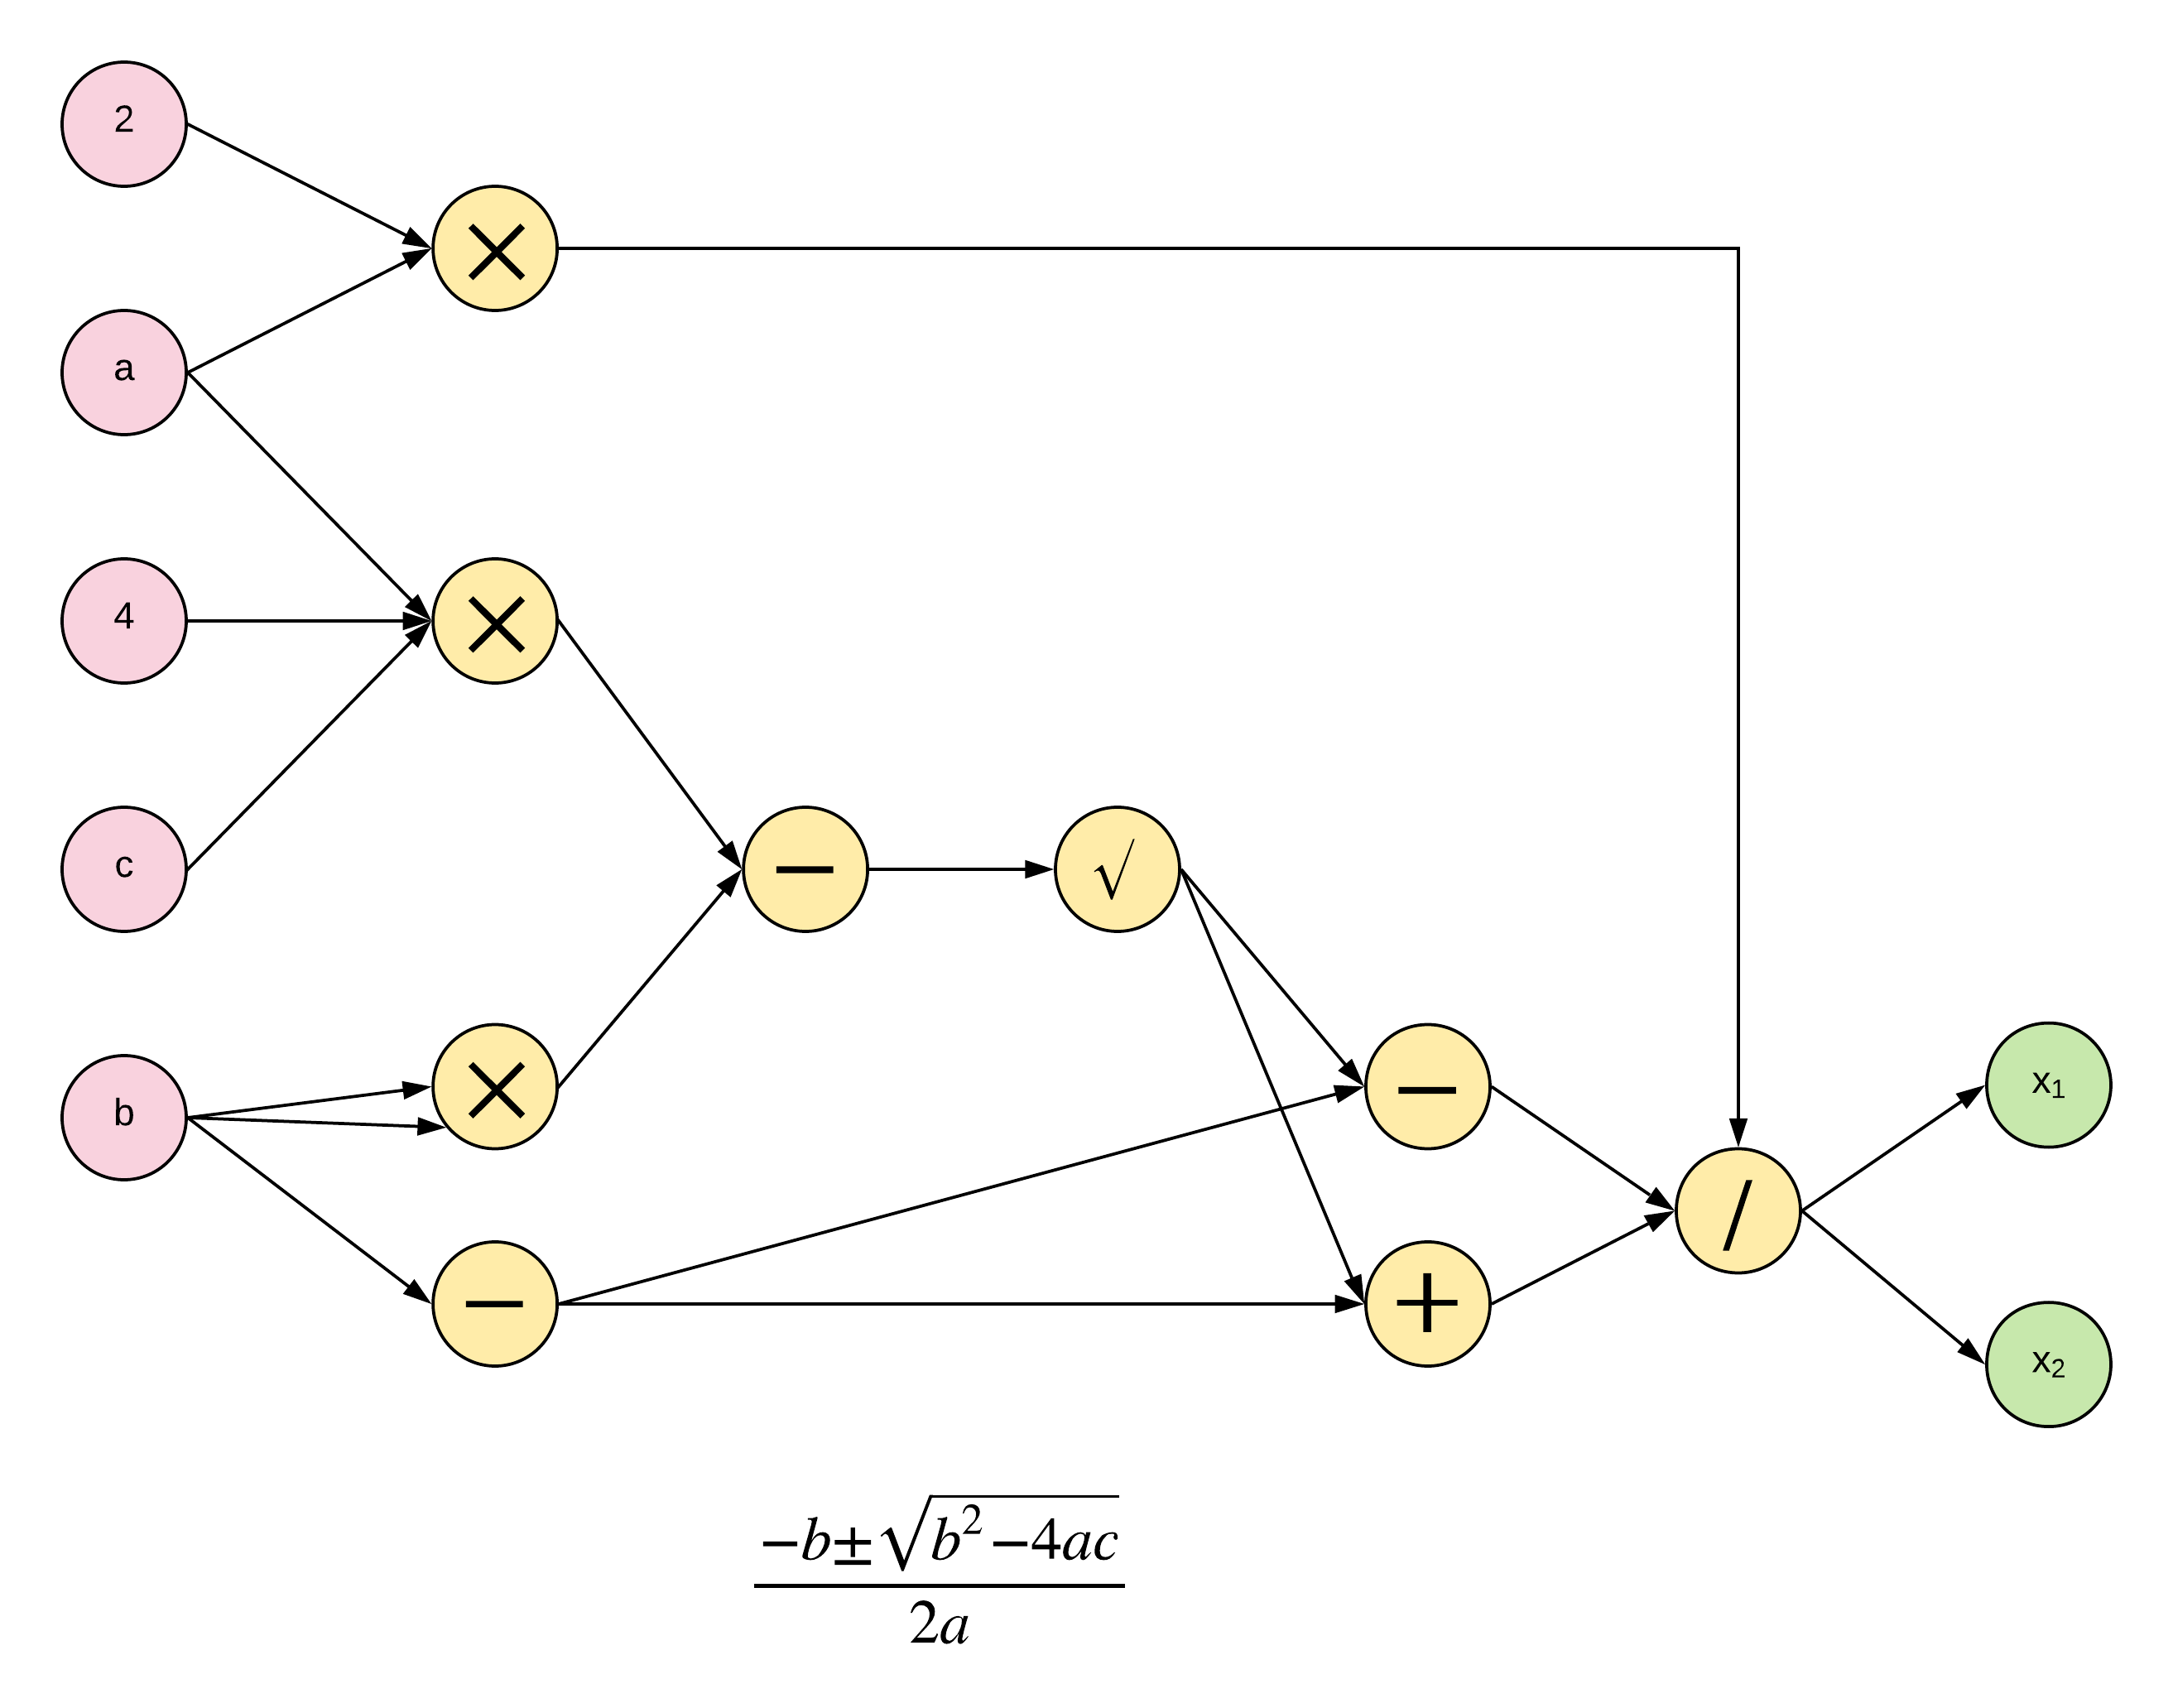
\includegraphics[height=0.5\textheight]{Figs/computational_graph.png}
		\caption{An example of computational graph, \href{https://ekababisong.org/gcp-ml-seminar/tensorflow/}{Source}.}
	\end{figure}
\end{frame}

\begin{frame}{Backward Propagation}
	\begin{itemize}
		\item In this approach if we know how to calculate gradient for single node or module, then we can find gradient with respect to each variables.
		\item Let's say we have a module as follow:
		\begin{figure}[H]
			\centering
			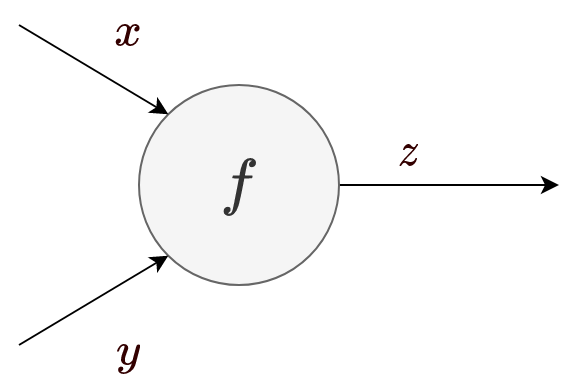
\includegraphics[width=0.35\textwidth]{Figs/module_f.png}
		\end{figure}
		\item It gets $x$ and $y$ as its input and returns $z = f(x, y)$ as its output.
		\item How to calculate derivative of loss with respect to module inputs?
	\end{itemize}
\end{frame}

\begin{frame}{Backward Propagation}
	\begin{itemize}
		\item We know:
		\begin{itemize}
			\item Module output for $x_0$ and $y_0$, let's call it $z_0$.
			\item Gradient of loss with respect to module output at $z_0$, $\left(\frac{\partial L}{\partial z}\right)$.
		\end{itemize}
		\item We want:
		\begin{itemize}
			\item Gradient of loss with respect to module inputs at $x_0$ and $y_0$, $\left(\frac{\partial L}{\partial x}, \frac{\partial L}{\partial y}\right)$.
		\end{itemize}
	\end{itemize}
	\begin{figure}[H]
		\centering
		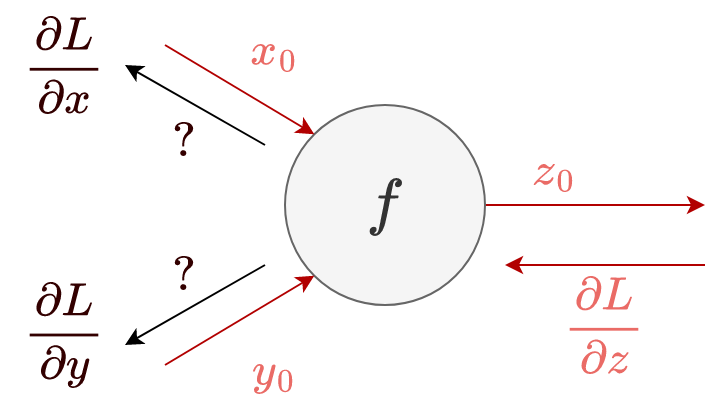
\includegraphics[width=0.4\textwidth]{Figs/module_f_upstream.png}
	\end{figure}
\end{frame}

\begin{frame}{Backward Propagation}
	\begin{itemize}
		\item We can use chain rule to do so.
		\medskip
		\begin{block}{Chain rule:}
			\[
			\left.\begin{aligned}
				& z = f(x, y)\\
				& L = L(z)
			\end{aligned}\right\}\quad\implies\quad \frac{\partial L}{\partial x} = \frac{\partial L}{\partial z}\times \frac{\partial z}{\partial x} 
			\]
		\end{block}
	\end{itemize}
	\begin{figure}[H]
		\centering
		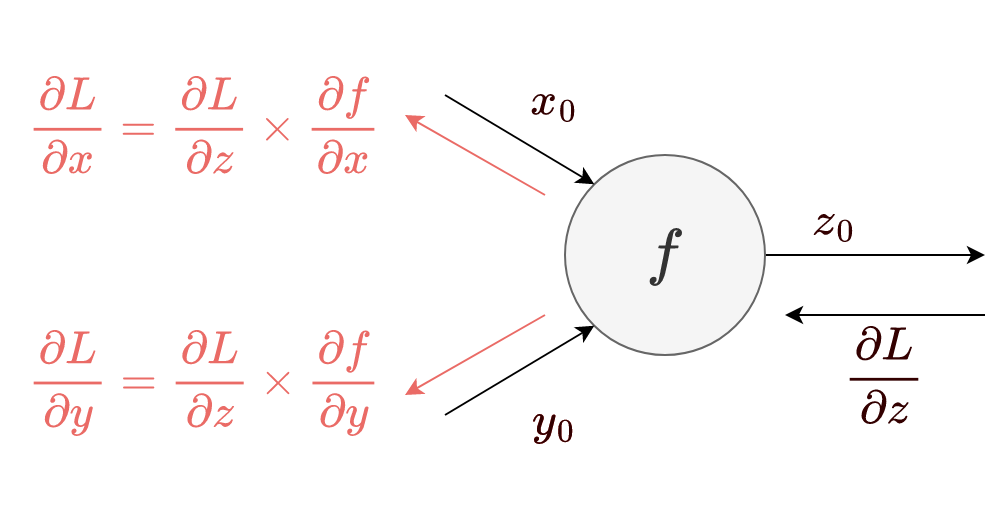
\includegraphics[width=0.6\textwidth]{Figs/module_f_downstream.png}
	\end{figure}
\end{frame}

\begin{frame}{Backward Propagation}
	\begin{itemize}
		\item Backpropagation for single module:
	\end{itemize}
	\begin{figure}[H]
		\centering
		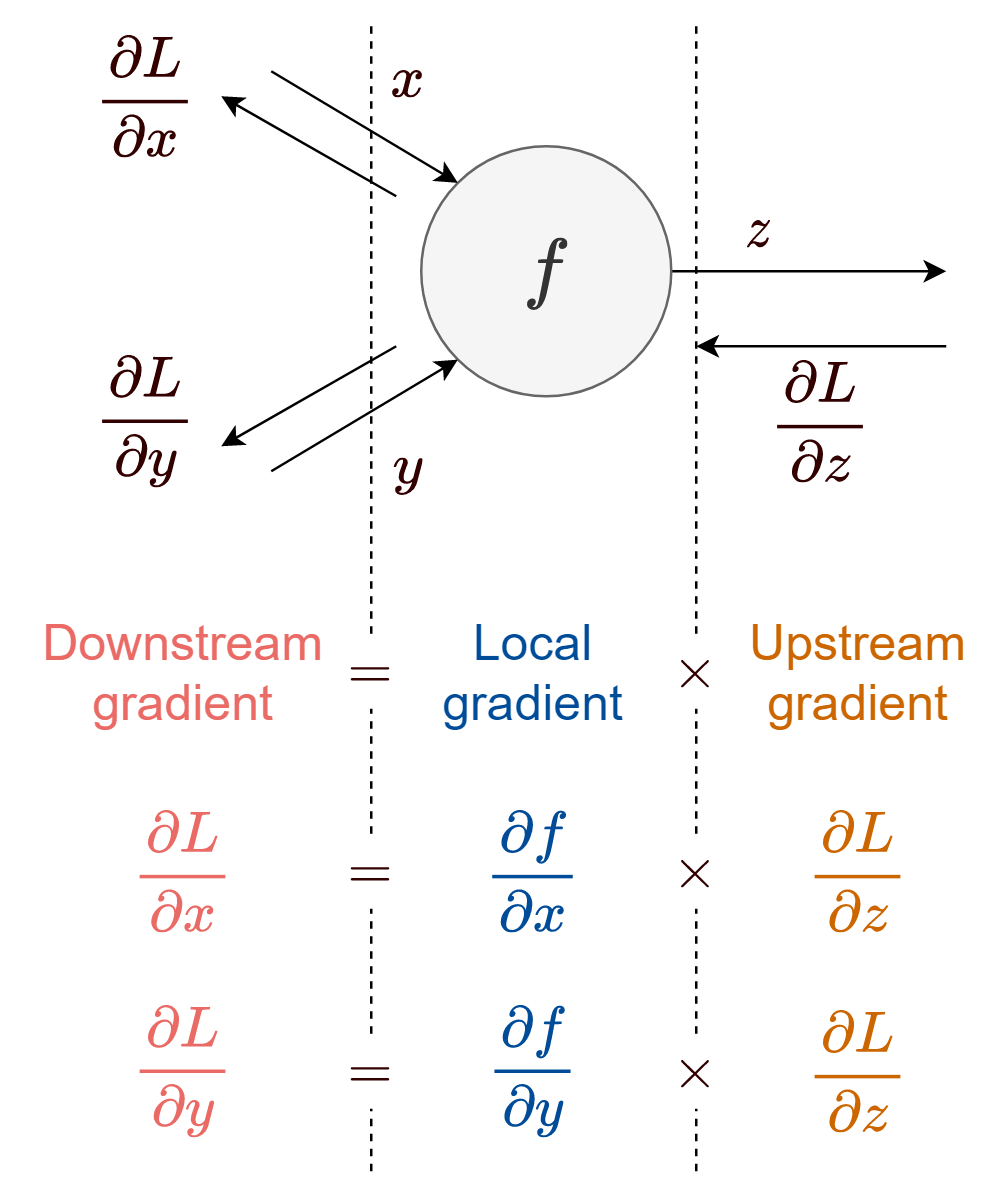
\includegraphics[height=0.7\textheight]{Figs/module_f_chain_rule.png}
	\end{figure}
\end{frame}

\begin{frame}{Backward Propagation: Example}
	\begin{itemize}
		\item Let's solve a simple example using backpropagation.
		\medskip
		\item We have $f(x, y, z) = \frac{x^2 y}{z}$.
		\medskip
		\item Find $\frac{\partial f}{\partial x}$, $\frac{\partial f}{\partial y}$ and $\frac{\partial f}{\partial z}$ at $x=3$, $y=4$ and $z=2$.
		\medskip
	\end{itemize}
	\begin{figure}[H]
		\centering
		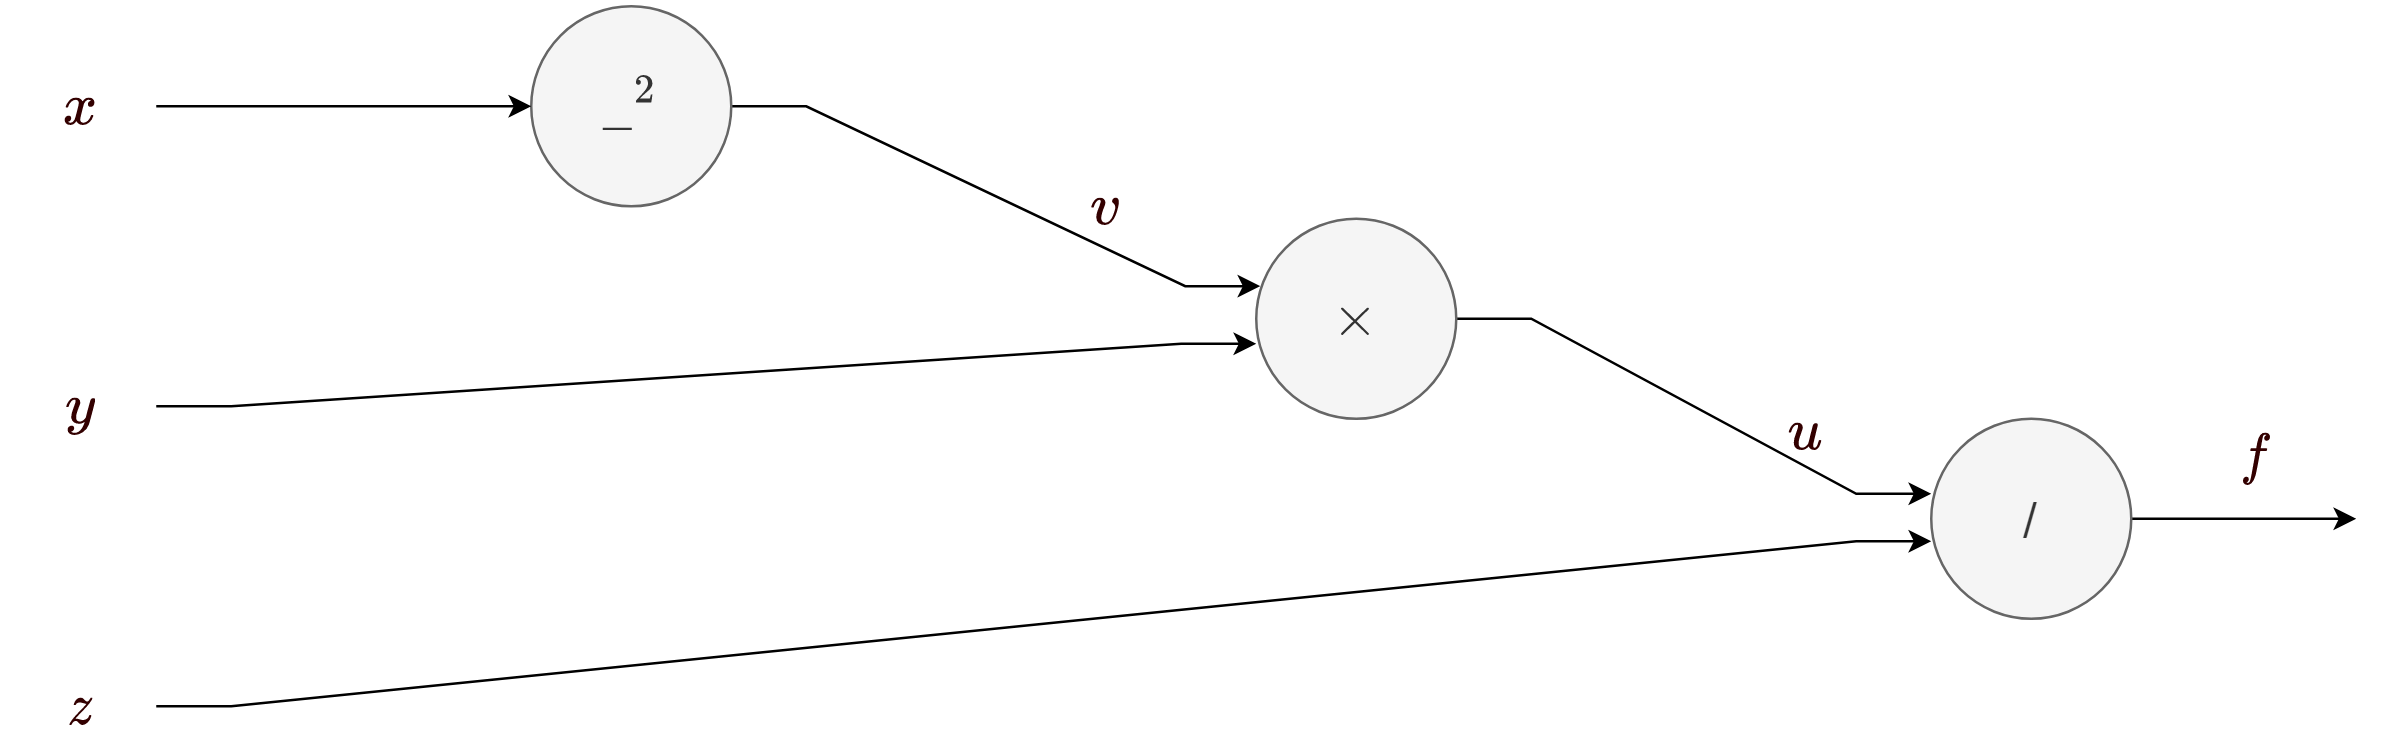
\includegraphics[width=0.9\textwidth]{Figs/backprop_e1.png}
		\caption{Computational graph of $f$.}
	\end{figure}
\end{frame}

\begin{frame}{Backward Propagation: Example}
	\begin{itemize}
		\item First let's find gradient analytically.
		\item We have:
		\[
		\begin{cases}
			v = x^2\\
			u = vy\\
			f = \frac{u}{z}
		\end{cases}
		\qquad
		\begin{cases}
			\frac{\partial f}{\partial z} = -\frac{u}{z^2}\\[0.7em]
			\frac{\partial f}{\partial y} = \frac{\partial u}{\partial y}\times\frac{\partial f}{\partial u} =  v \times \frac{1}{z} = \frac{v}{z}\\[0.7em]
			\frac{\partial f}{\partial x} = \frac{\partial v}{\partial x}\times\frac{\partial u}{\partial v}\times\frac{\partial f}{\partial u} = 2x \times y \times \frac{1}{z} = \frac{2xy}{z}
		\end{cases}
		\]
		\[
		(x=3, y=4, z=2)\implies
		\begin{cases}
			v = 9\\
			u = 36 \\
			f = 18
		\end{cases}
		\implies
		\begin{cases}
			\frac{\partial f}{\partial z} = -9\\[0.7em]
			\frac{\partial f}{\partial y} = 4.5\\[0.7em]
			\frac{\partial f}{\partial x} = 12
		\end{cases}
		\]
	\end{itemize}
\end{frame}

\begin{frame}{Backward Propagation: Example}
	\begin{itemize}
		\item Now let's use backpropagation.
		\item First we do forward propagation.
		\medskip
		\begin{figure}[H]
			\centering
			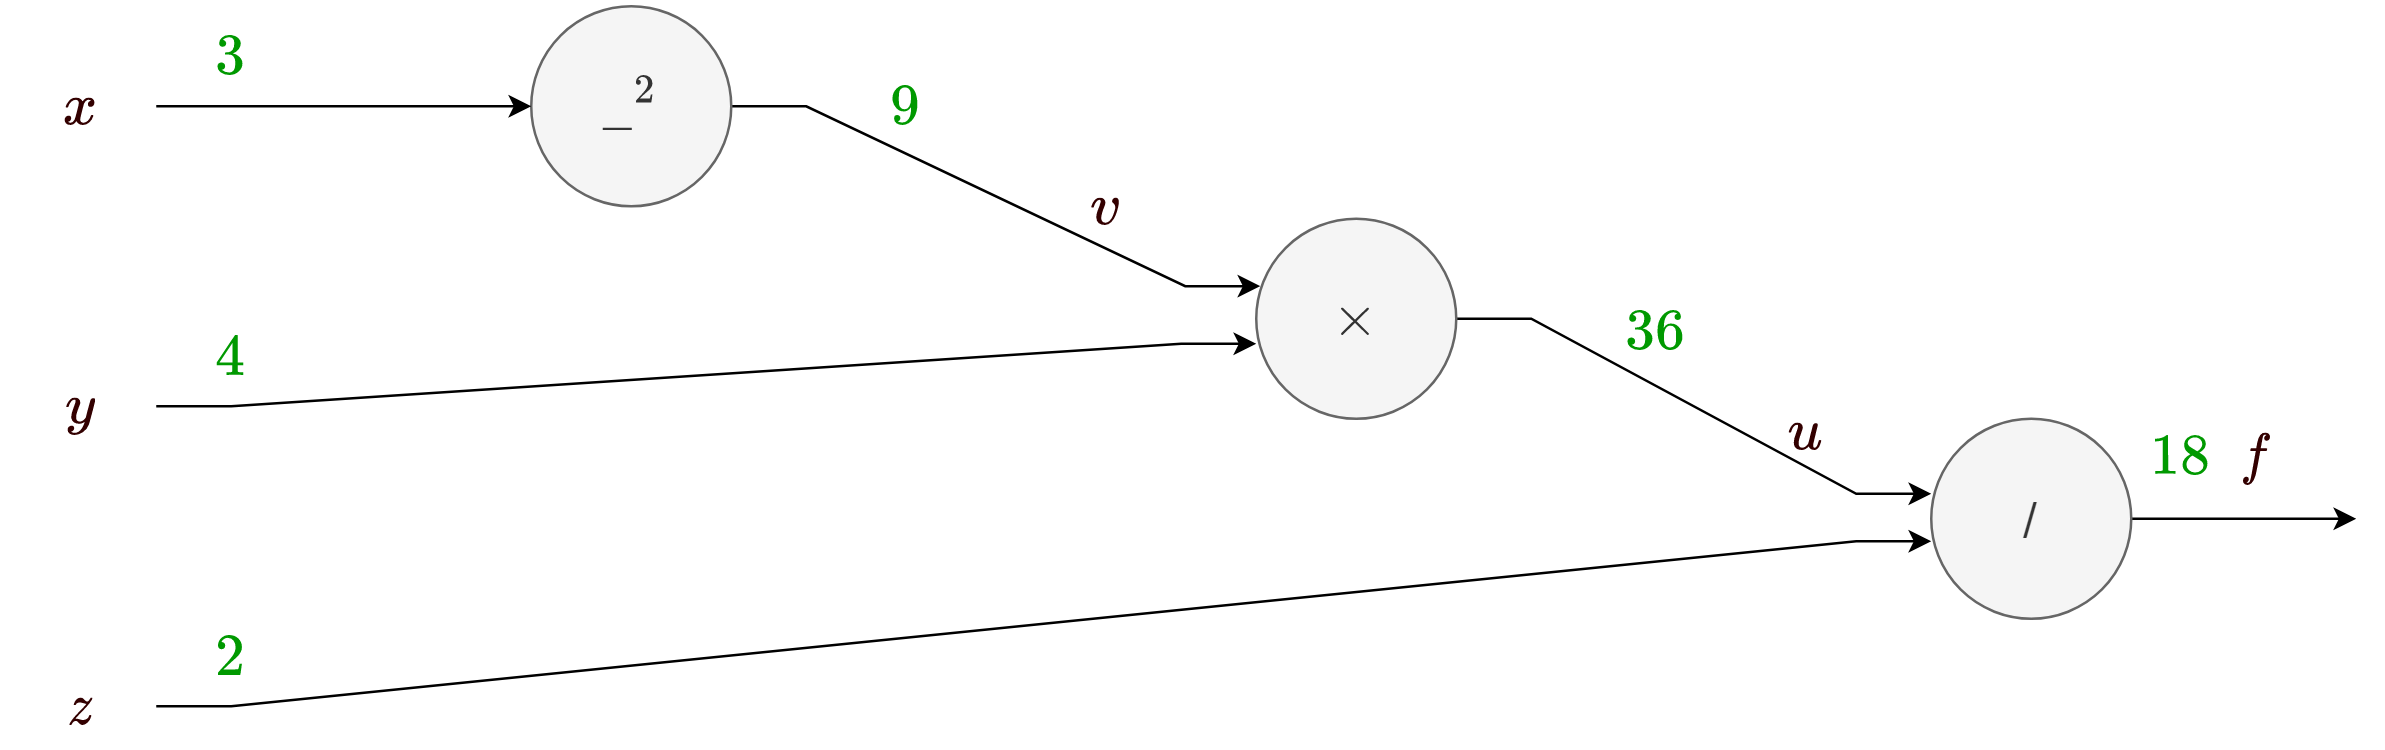
\includegraphics[width=0.9\textwidth]{Figs/backprop_e2.png}
		\end{figure}
		\medskip
		\item Second we will do backpropagation for each module.
	\end{itemize}
\end{frame}

\begin{frame}{Backward Propagation: Example}
	\begin{itemize}
		\item Backpropagation for $/$ module:
	\end{itemize}
	\begin{figure}[H]
		\centering
		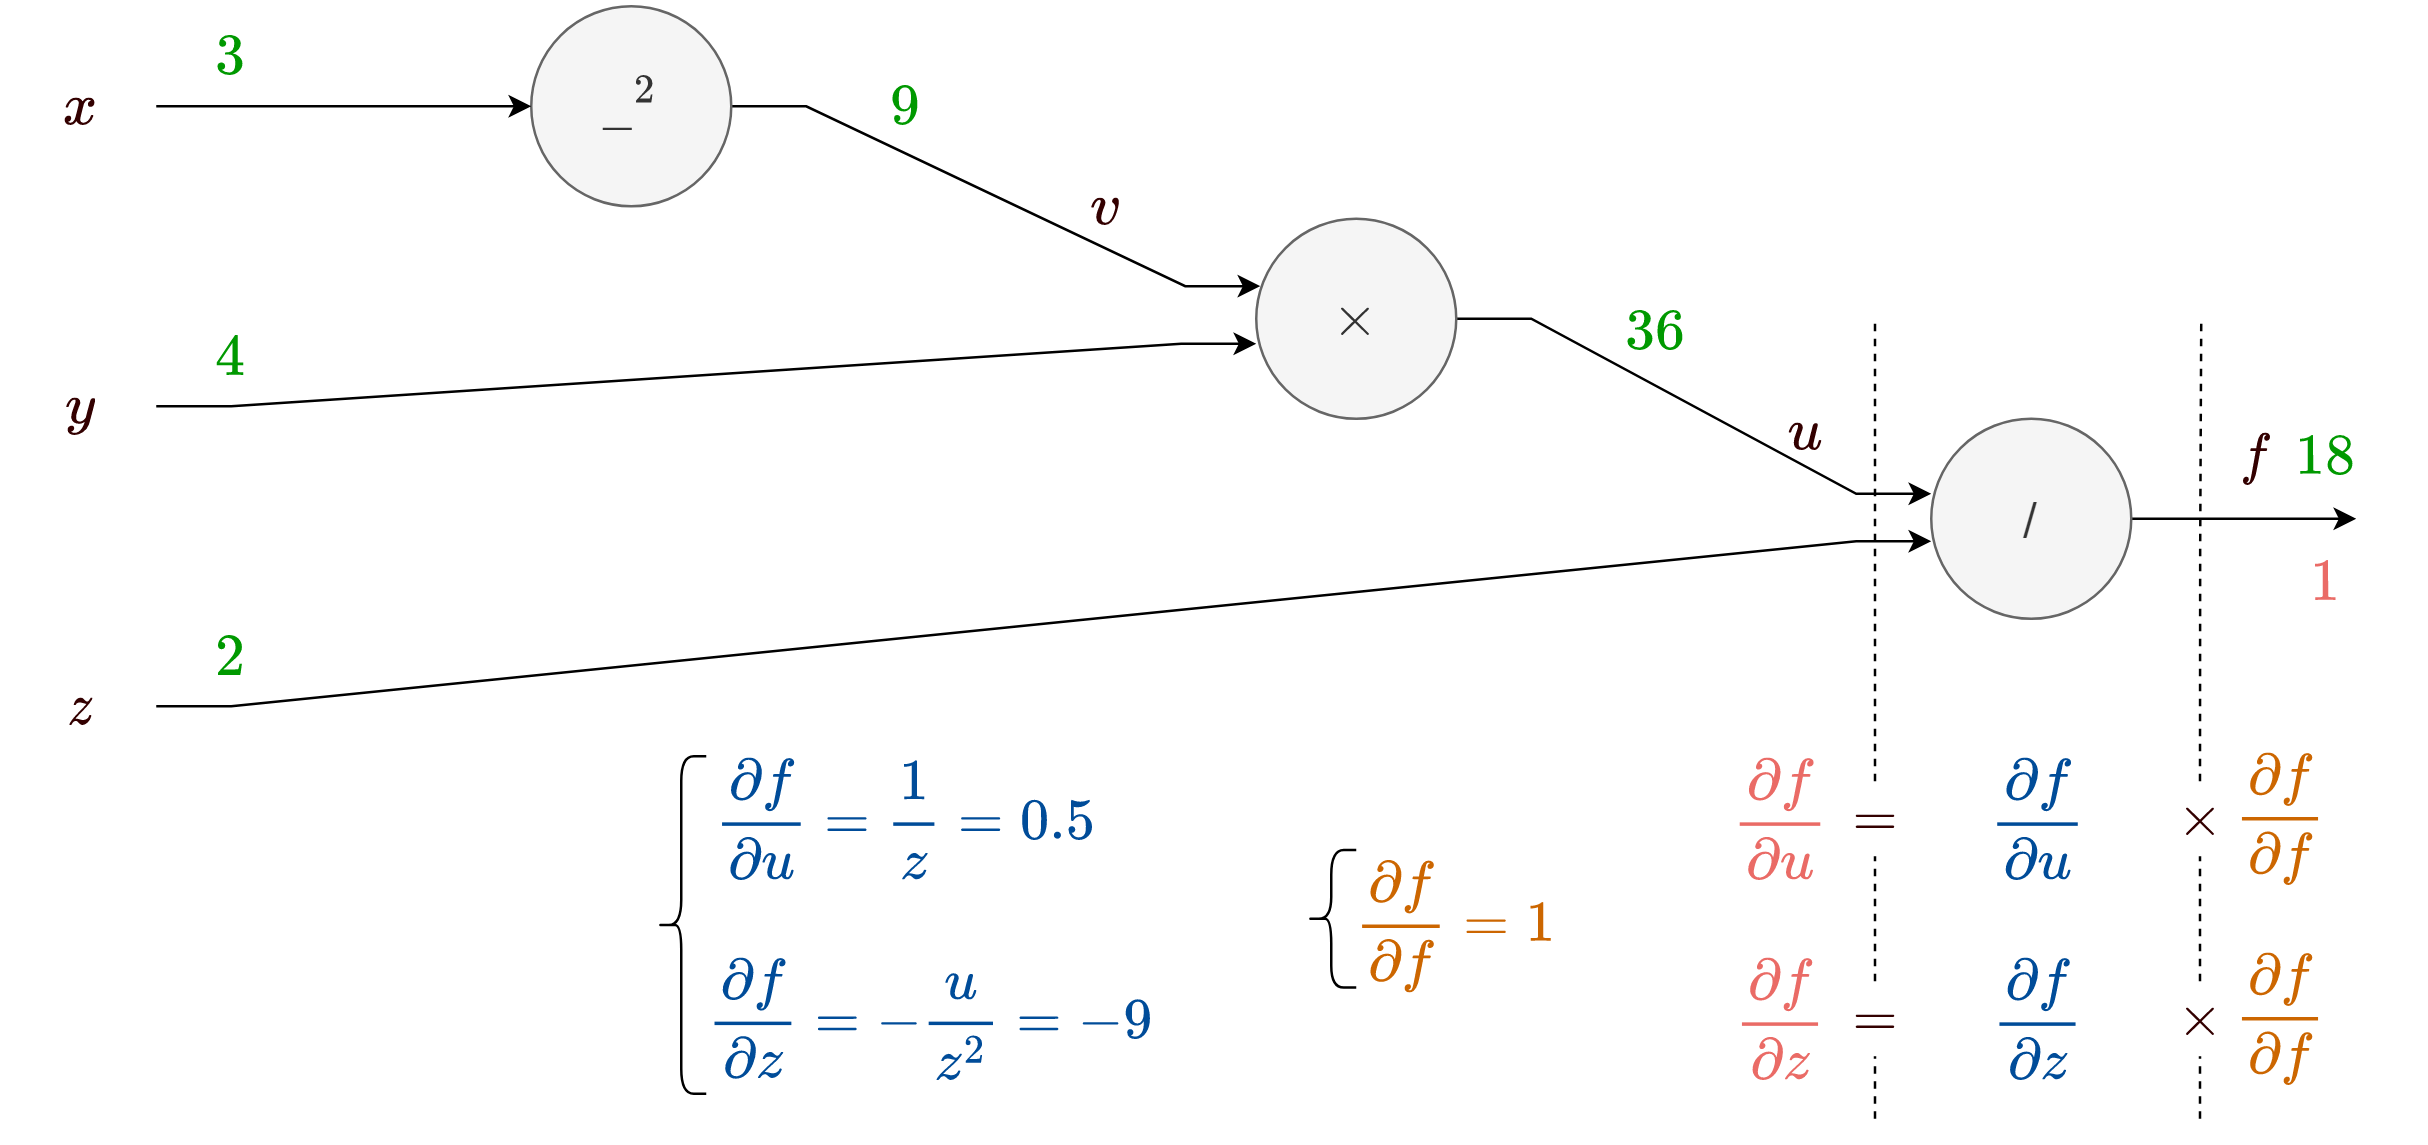
\includegraphics[width=0.9\textwidth]{Figs/backprop_e3.png}
	\end{figure}
\end{frame}

\begin{frame}{Backward Propagation: Example}
	\begin{itemize}
		\item Backpropagation for $/$ module:
	\end{itemize}
	\begin{figure}[H]
		\centering
		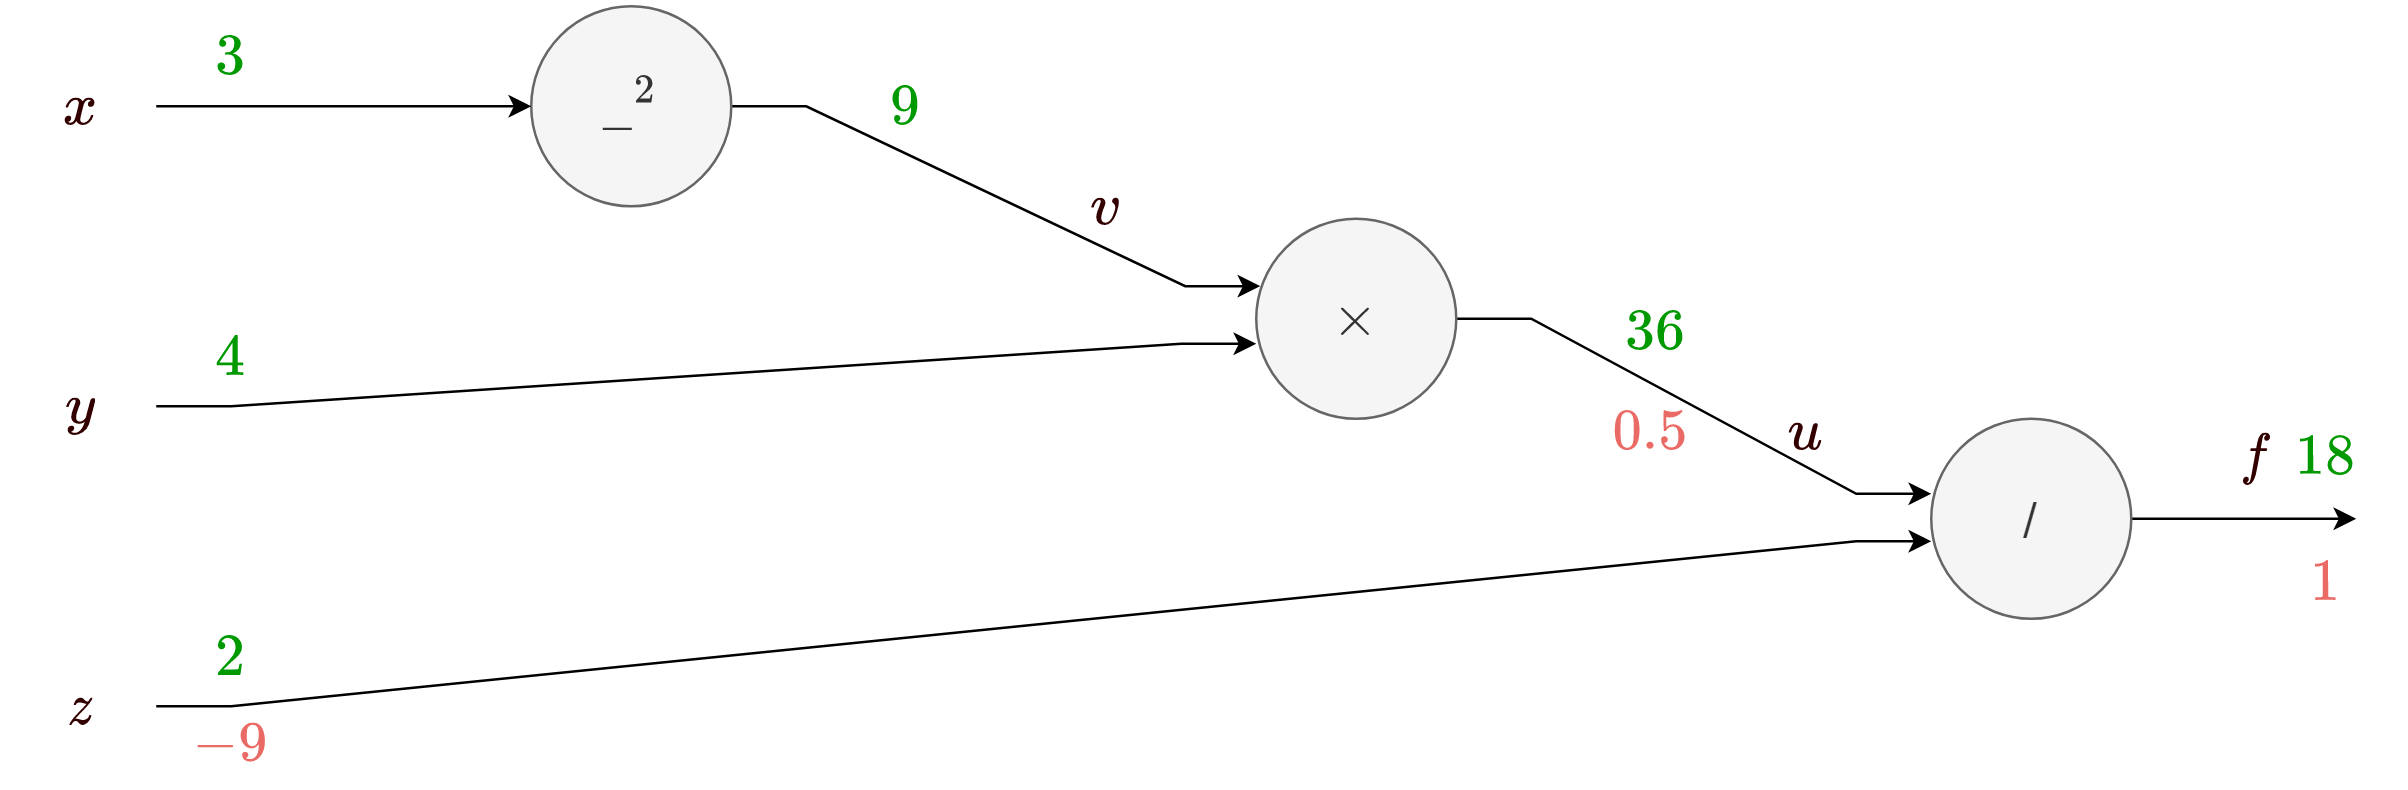
\includegraphics[width=0.9\textwidth]{Figs/backprop_e4.png}
	\end{figure}
\end{frame}

\begin{frame}{Backward Propagation: Example}
	\begin{itemize}
		\item Backpropagation for $\times$ module:
	\end{itemize}
	\begin{figure}[H]
		\centering
		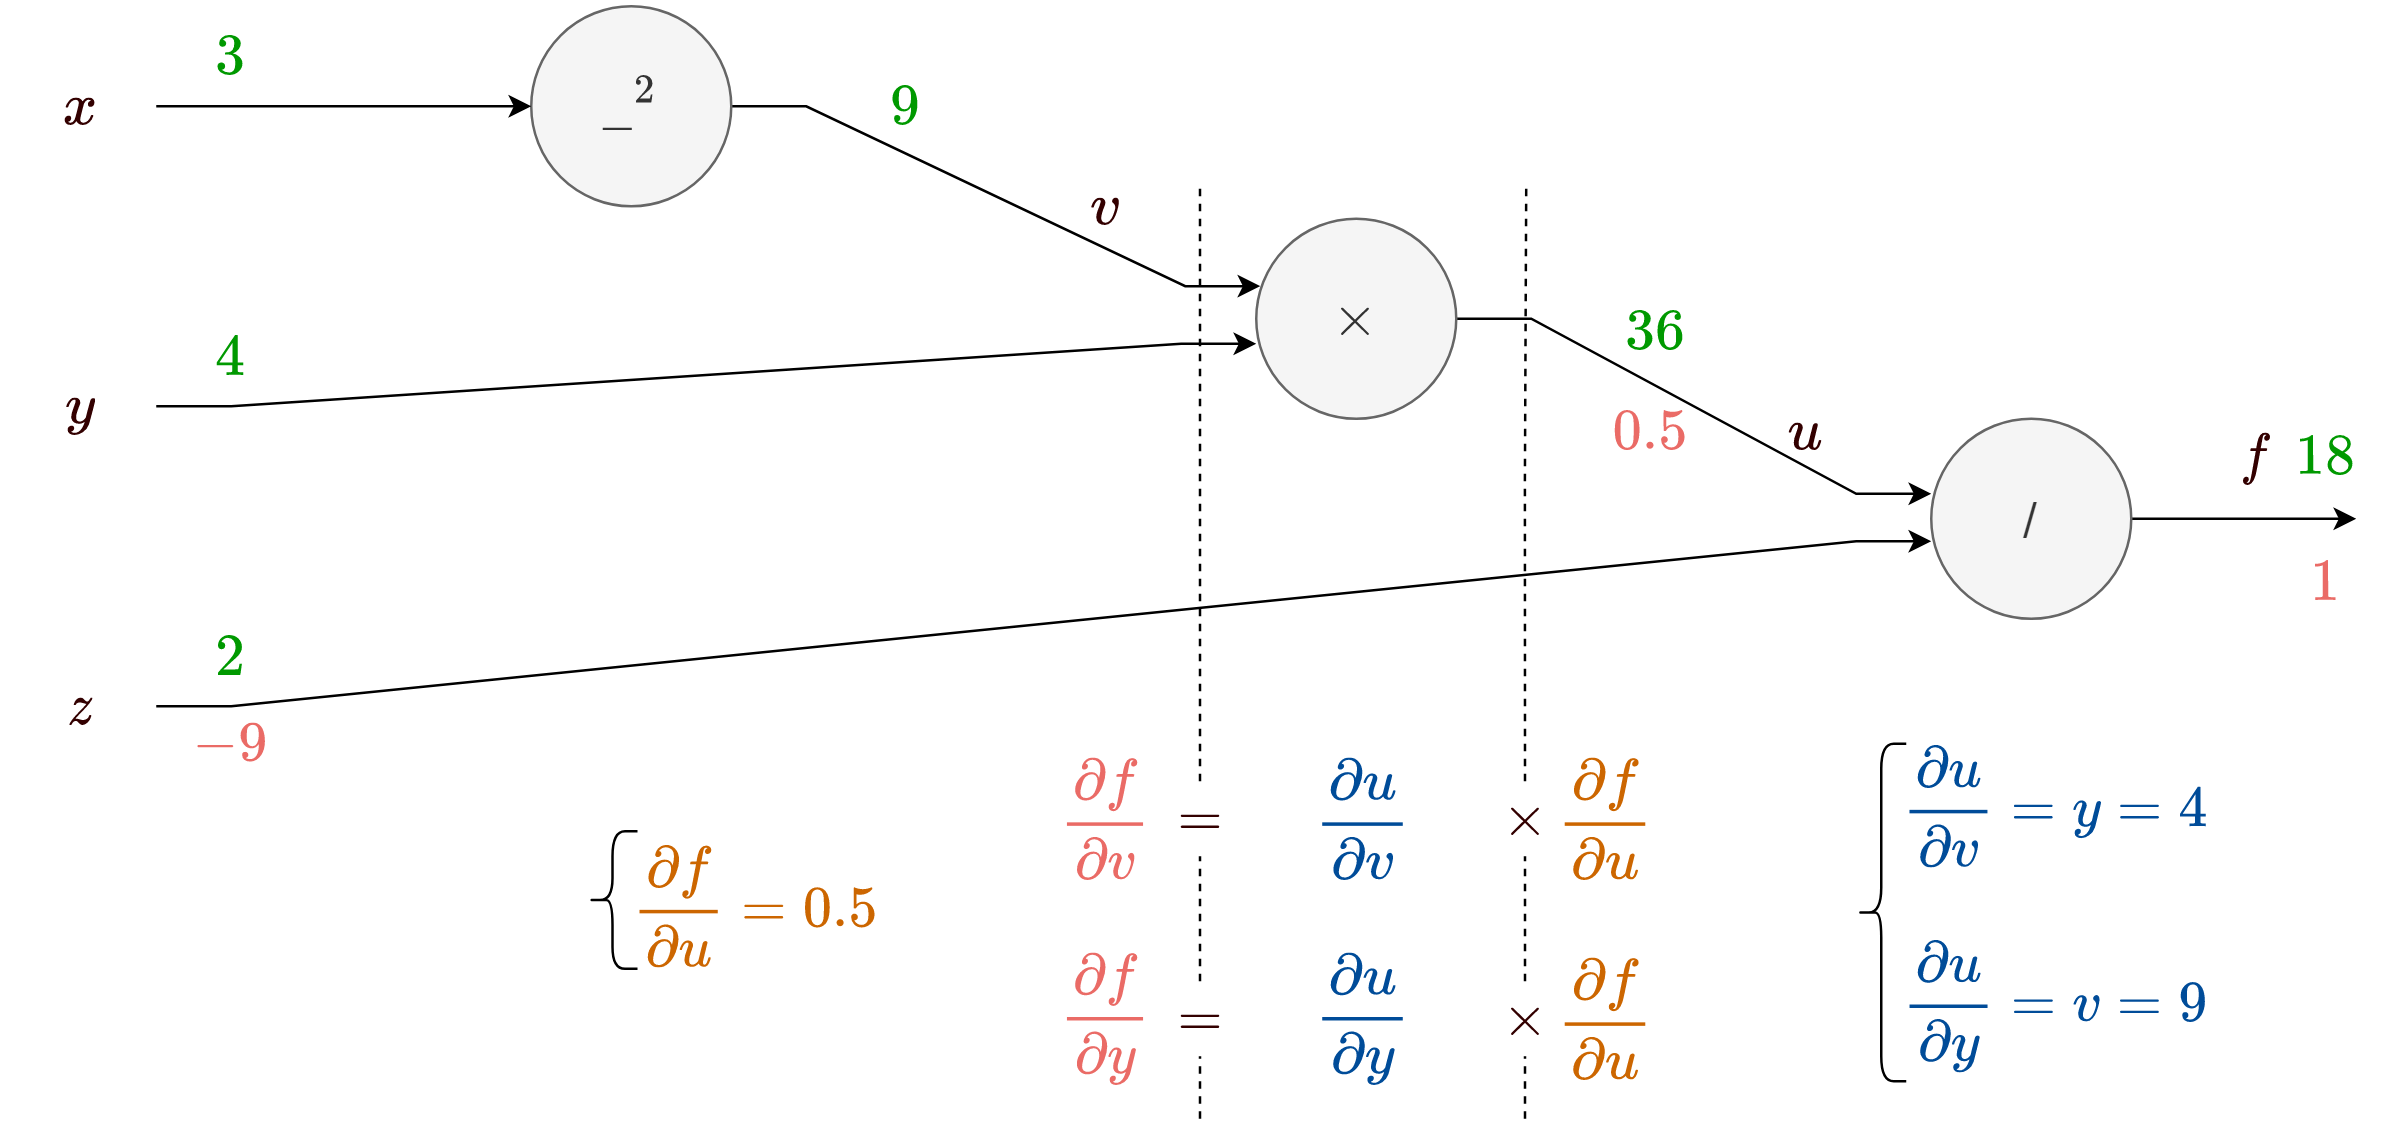
\includegraphics[width=0.9\textwidth]{Figs/backprop_e5.png}
	\end{figure}
\end{frame}

\begin{frame}{Backward Propagation: Example}
	\begin{itemize}
		\item Backpropagation for $\times$ module:
	\end{itemize}
	\begin{figure}[H]
		\centering
		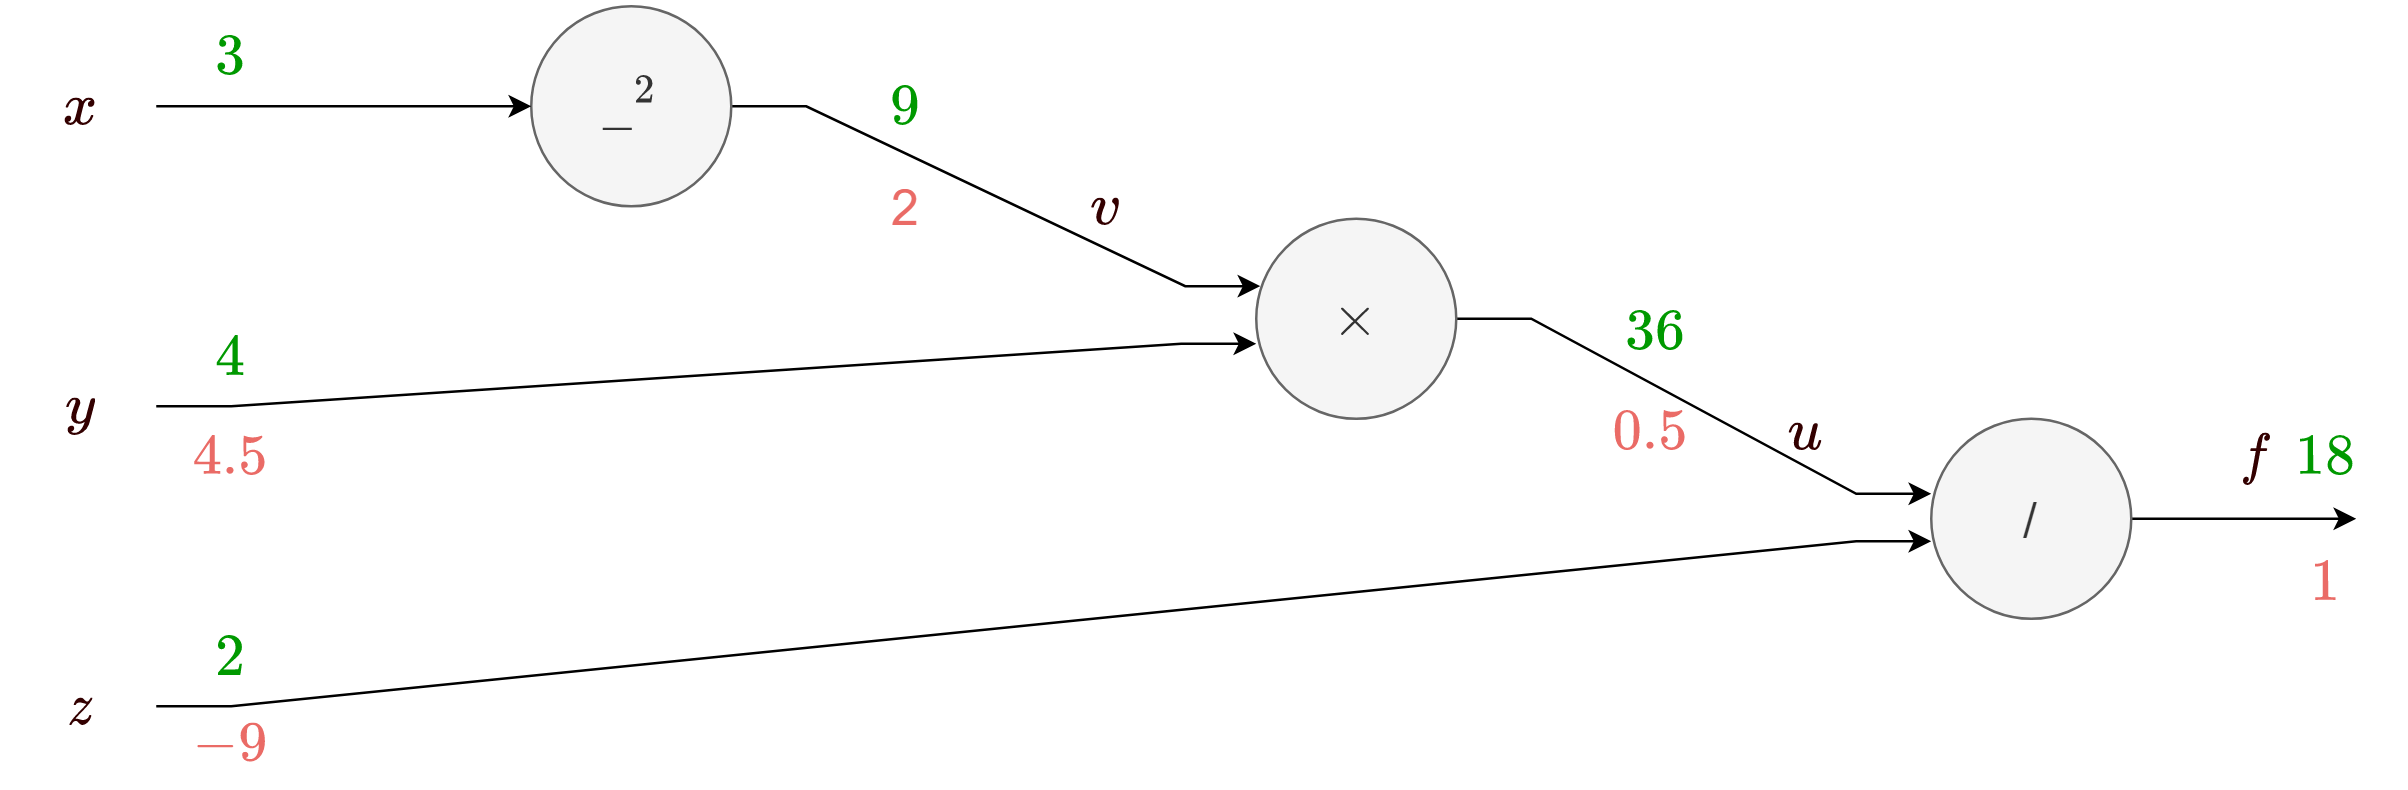
\includegraphics[width=0.9\textwidth]{Figs/backprop_e6.png}
	\end{figure}
\end{frame}

\begin{frame}{Backward Propagation: Example}
	\begin{itemize}
		\item Backpropagation for ${\_}^2$ module:
	\end{itemize}
	\begin{figure}[H]
		\centering
		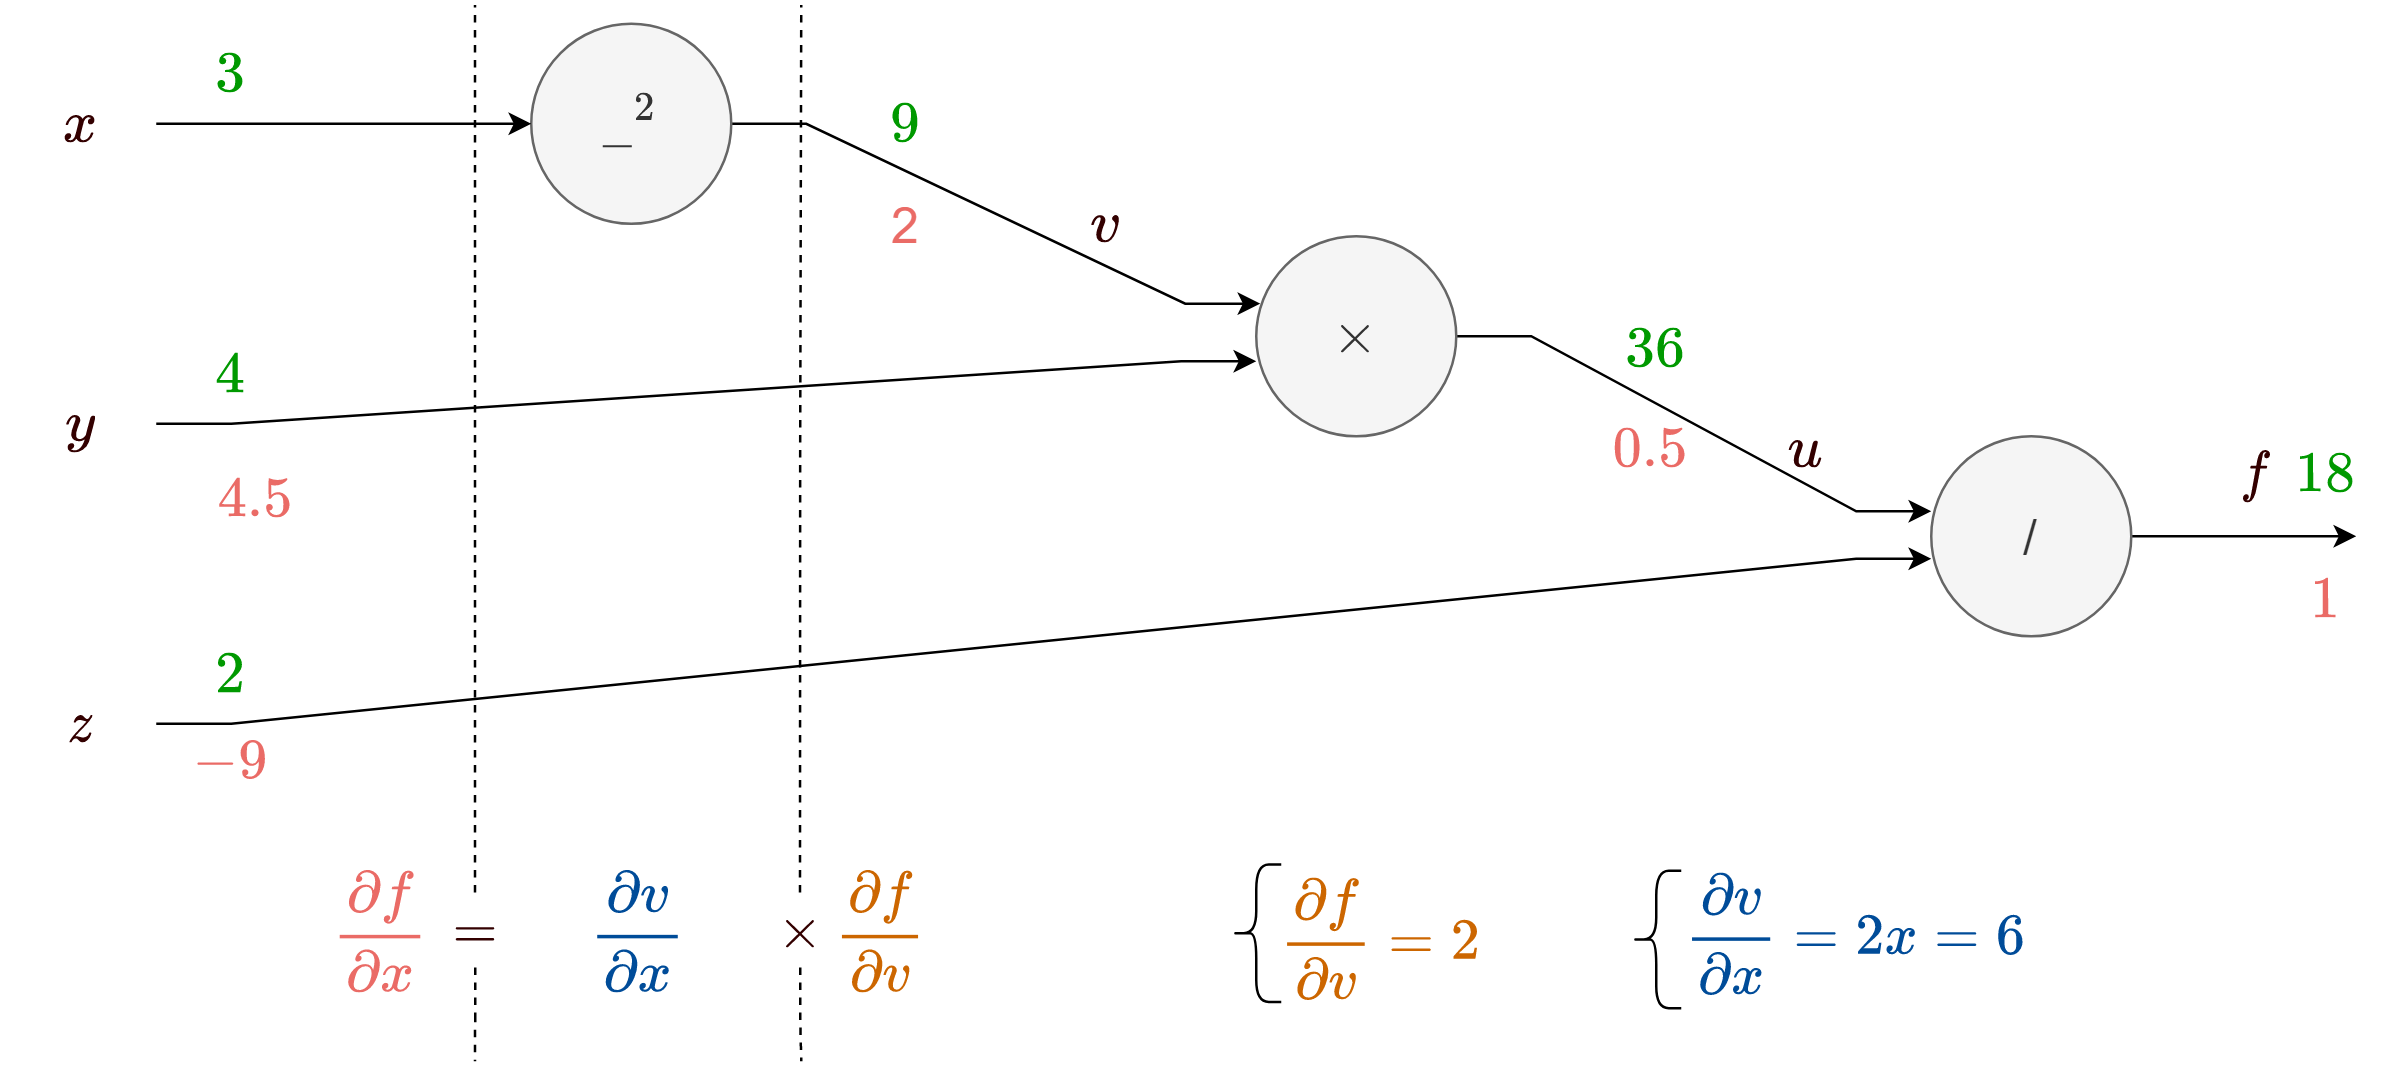
\includegraphics[width=0.9\textwidth]{Figs/backprop_e7.png}
	\end{figure}
\end{frame}

\begin{frame}{Backward Propagation: Example}
	\begin{itemize}
		\item Backpropagation for ${\_}^2$ module:
	\end{itemize}
	\begin{figure}[H]
		\centering
		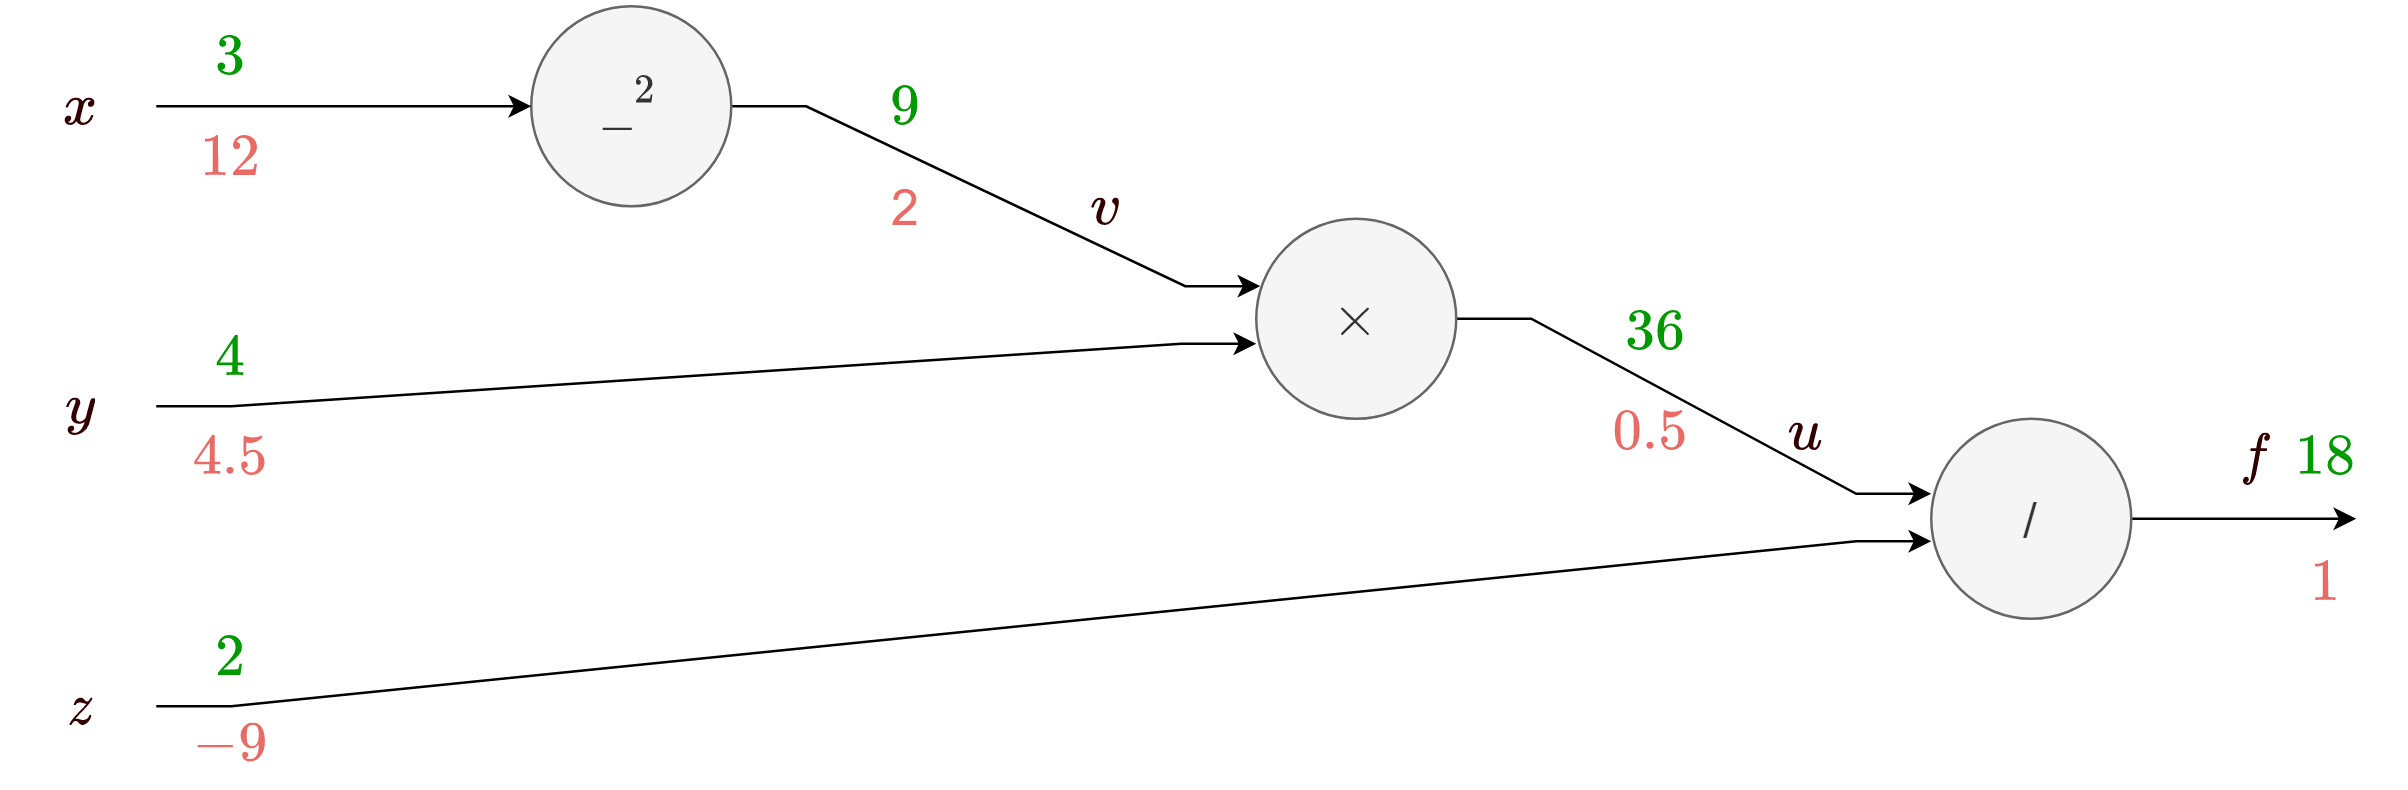
\includegraphics[width=0.9\textwidth]{Figs/backprop_e8.png}
	\end{figure}
	\begin{itemize}
		\item Results are the same as analytical results.
	\end{itemize}
\end{frame}

\begin{frame}{Backward Propagation}
	\begin{itemize}
		\item So after backward propagation we will have:
		\begin{itemize}
			\item Gradient of loss with respect to each parameter.
			\item We can apply gradient descent to update parameters.
		\end{itemize}
	\end{itemize}
	\begin{figure}[H]
		\includegraphics[width=0.5\textwidth]{Figs/backward_propagation.png}
		\caption{Backward pass}
	\end{figure}
\end{frame}


%%%%%%%%%%%%%%%%%%%%%%%%%%[Stochastic Gradient Descent]%%%%%%%%%%%%%%%%%%%%%%%%%%%%%%%%%%%%%%%%%%%
\section{Stochastic Gradient Descent}
\begin{frame}{Various GD types}
	\begin{itemize}
		\item So far you got familiar with gradient-based optimization.
		\item If $\bm{g} = \nabla_{\bm{\theta}} \mathcal{J}$, then we will update parameters with this simple rule:
		\[
		\bm{\theta} \gets \bm{\theta} - \eta\bm{g}
		\]
		% 	\item[]
		\item But there is one question here, how to compute $\bm{g}$?
		\item Based on how we calculate $\bm{g}$ we will have different types of gradient descent:
		\begin{itemize}
			\item Batch Gradient Descent
			\item Stochastic Gradient Descent
			\item Mini-Batch Gradient Descent
		\end{itemize}
	\end{itemize}
\end{frame}

\begin{frame}{Various GD types}
	\begin{block}{Recap:}
		Training cost function ($\mathcal{J}$) over a dataset usually is the average of loss function ($\mathcal{L}$) on entire training set, so for a dataset $\mathcal{D}=\{d_i\}_{i=1}^n$ we have:
		\[
		\mathcal{J}(\mathcal{D}) = \frac{1}{n} \sum_{i=1}^{n} \mathcal{L}(d_i; \bm{\theta})
		\]
		For example:
		\begin{equation*}
			H(p, q)=-\frac{1}{m} \sum_{i=1}^m\sum_{j=1}^{k} y_j^{(i)} \log (p(y_j^{(i)}))
		\end{equation*}
		\begin{equation*}
			\text{MSE}(y, \hat{y}) = \frac{1}{m}\sum_{i=1}^{m}(y_i-\hat{y}_i)^2
		\end{equation*}
		\begin{equation*}
			\text{MAE}(y, \hat{y}) = \frac{1}{m}\sum_{i=1}^{m}|(y_i-\hat{y}_i)|
		\end{equation*}
	\end{block}
\end{frame}

\begin{frame}{Various GD types: Batch Gradient Descent}
	\begin{itemize}
		\item In this type we use \tc{keywords}{entire training set} to calculate gradient.
		\begin{block}{Batch Gradient:}
			\[
			\bm{g} = \frac{1}{n}\sum_{i=1}^n \nabla_{\bm{\theta}} \mathcal{L}(d_i, \bm{\theta})
			\]
		\end{block}
		\item[]
		\item Using this method with very large training set:
		\begin{itemize}
			\item Your data can be too large to process in your memory.
			\item It requires a lot of processing to compute gradient for all samples.
		\end{itemize}
		\item Using exact gradient may lead us to local minima.
		\item Moving noisy may help us get out of this local minimas.
	\end{itemize}
\end{frame}

\begin{frame}{Various GD types: Batch Gradient Descent}
	\begin{figure}[H]
		\centering
		\includegraphics[width=0.8\textwidth]{Figs/bgd.png}
		\caption{Optimization of parameters using BGD. Movement is very smooth \cite{katanforoosh-kunin-opt}.}
	\end{figure} 
\end{frame}

\begin{frame}{Various GD types: Stochastic Gradient Descent}
	\begin{itemize}
		\item Instead of calculating exact gradient, we can estimate it using our data.
		\item This is exactly what SGD does, it estimates gradient using \tc{keywords}{only single data point}.
		\begin{block}{Stochastic Gradient:}
			\[
			\hat{\bm{g}} = \nabla_{\bm{\theta}} \mathcal{L}(d_i, \bm{\theta})
			\]
		\end{block}
		\item[]
		\item As we use an approximation of gradient, instead of gently decreasing, the cost function will bounce up and down and decrease only on average.
		\item This method is really computationally efficient cause we only need to calculate gradient for one point per iteration. 
	\end{itemize}
\end{frame}

\begin{frame}{Various GD types: Stochastic Gradient Descent}
	\begin{figure}[H]
		\centering
		\includegraphics[width=0.8\textwidth]{Figs/sgd.png}
		\caption{Optimization of parameters using SGD. As we expect, the movement is not that smooth \cite{katanforoosh-kunin-opt}.}
	\end{figure} 
\end{frame}

\begin{frame}{Various GD types: Mini-Batch Gradient Descent}
	\begin{itemize}
		\item In this method we still use estimation idea But use \tc{keywords}{a batch of data} instead of one point.
		\begin{block}{Mini-Batch Gradient:}
			\[
			\hat{\bm{g}} = \frac{1}{|\mathcal{B}|} \sum_{d\in\mathcal{B}} \nabla_{\bm{\theta}} \mathcal{L}(d, \bm{\theta}), \quad \mathcal{B} \subset \mathcal{D}
			\]
		\end{block}
		\item[]
		\item This is a better estimation than SGD.
		\item With this way we can get a performance boost from hardware optimization, especially when using GPUs.
		\item Batch size ($|\mathcal{B}|$) is a hyperparameter you need to tune.
	\end{itemize}
\end{frame}

\begin{frame}{Various GD types: Mini-Batch Gradient Descent}
	\begin{figure}[H]
		\centering
		\includegraphics[width=0.8\textwidth]{Figs/mbgd.png}
		\caption{Optimization of parameters using MBGD. The movement is much smother than SGD and behaves like BGD \cite{katanforoosh-kunin-opt}.}
	\end{figure} 
\end{frame}

\begin{frame}{Various GD types}
	\begin{itemize}
		\item Now that we know what a batch is, we can define epoch and iteration:
		\begin{itemize}
			\item One \tc{keywords}{Epoch} is when an entire dataset is passed forward and backward through the network only once.
			\item One \tc{keywords}{Iteration} is when a batch is passed forward and backward through the network. 
		\end{itemize}
		
		\begin{figure}[H]
			\centering
			\includegraphics[width=0.4\textwidth]{Figs/epoch-iteration.png}
			\caption{Epoch vs Iteration, \href{https://jerryan.medium.com/batch-size-a15958708a6}{source}.}
		\end{figure} 
	\end{itemize}
\end{frame}

\begin{frame}{Various GD types}
	\begin{itemize}
		\item So we got familiar with different types of GD.
		\begin{itemize}
			\item[\color{darkgreen}$\checkmark$] Batch Gradient Descent (BGD)
			\item[\color{darkgreen}$\checkmark$] Stochastic Gradient Descent (SGD)
			\item[\color{darkgreen}$\checkmark$] Mini-Batch Gradient Descent (MBGD)
		\end{itemize}
		\item[]
		\item[]
		\item The most recommended one is MBGD, because it is computationally efficient.
		\item Choosing the right batch size is important to ensure convergence of the cost function and parameter values, and to the generalization of your model.
	\end{itemize}
\end{frame}

\section{Training MLPs}
\begin{frame}{Training MLPs}
	\begin{itemize}
		\item So far we have learned about how MLPs work and how to update their parameters in order to perform better.
		\item But training MLPs is not that easy.
		\item You will face several different challenges in this procedure.
		\item In this section we will talk about this challenges and how to solve them.
	\end{itemize}
\end{frame}


%%%%%%%%%%%%%%%%%%%%%%%%[Vanishing Exploding]%%%%%%%%%%%%%%%%%%%%%%%%
\begin{frame}{Vanishing/Exploding Gradient}
	\begin{itemize}
		\item The backpropagation algorithm propagates the error gradient while proceeding from the output layer to the input layer. The issue here is the magnitude of the cost function gradients through the layers... 
	\end{itemize}
	\begin{figure}
		\centering
		\includegraphics[width=8cm, height=4cm]{Figs/van_2.png}
		\caption{Vanishing/Exploding Gradient, \href{https://medium.com/@ayushch612/vanishing-gradient-and-exploding-gradient-problems-7737c0aa535f}{Source}}
	\end{figure}
\end{frame}

\begin{frame}{Vanishing/Exploding Gradient}
	\begin{itemize}
		\item Vanishing
		\begin{itemize}
			\item Gradients often get smaller as the algorithm progresses down. As a result, gradient descent updates do not effectively change the weights of the lower layer connections, and training never converges.
			\medskip
			\item Make learning slow especially of front layers in the network.
			\medskip
		\end{itemize}
		\item Exploding
		\begin{itemize}
			\item Gradients can get bigger and bigger, so there are very large weight updates at many levels, causing the algorithm to diverge.
			\medskip
			\item The model is not learning much on the training data therefore resulting in a poor loss.
			\medskip
		\end{itemize}
	\end{itemize}
\end{frame}


%%%%%%%%%%%%%%%%%%%%%%%%%%%%%%%%[Weight Initialization]%%%%%%%%%%%%%%%%%%%%%%%%%%%%%%%%%%%
\begin{frame}{Weight Initialization}
	\begin{itemize}
		\item Is initialization really necessary?
		\item What are the impacts of initialization?
		\item A bad initialization may increase convergence time or even make optimization diverge.
		\item How to initialize?
		\begin{itemize}
			\item Zero initialization
			\item Random initialization
		\end{itemize}
	\end{itemize}
	\begin{figure}[H]
		\centering
		\includegraphics[width=0.65\textwidth]{Figs/wi-crucial.png}
		\caption{The output of a three layer network after about 600 epochs. (left) using a bad\\ initialization method and (right) using an appropriate initialization \cite{katanforoosh-kunin}.}
	\end{figure}
\end{frame}

\begin{frame}{Weight Initialization}
	\begin{block}{Let's review some notations before we continue:}
		\begin{columns}
			\begin{column}{0.4\textwidth}
				\[
				\begin{cases}
					n^{[l]} := \text{layer $l$ neurons number}, \\[0.5em]
					W^{[l]} := \text{layer $l$ weights},\\[0.5em]
					b^{[l]} := \text{layer $l$ biases},\\[0.5em]
					a^{[l]} := \text{layer $l$ outputs}
				\end{cases}
				\]
				\[
				\begin{cases}
					\text{fan}_\text{in}^{[l]} = n^{[l-1]} \quad (\text{layer $l$ number of inputs}),\\[0.6em]
					\text{fan}_\text{out}^{[l]} = n^{[l]} \quad (\text{layer $l$ number of outputs}),\\[0.6em]
					\text{fan}_\text{avg}^{[l]} = \frac{n^{[l-1]} + n^{[l]}}{2}
				\end{cases}
				\]
			\end{column}\hfill
			\begin{column}{0.4\textwidth}
				\begin{figure}[H]
					\centering	\includegraphics[width=0.65\textwidth]{Figs/notation_review.png}
				\end{figure}
			\end{column}
		\end{columns}
	\end{block}
\end{frame}

\begin{frame}{Weight Initialization: Zero Initialization}
	\begin{block}{Zero Initialization method:}
		\[
		\begin{cases}
			W^{[l]} = \bm{0},\\
			b^{[l]} = \bm{0}
		\end{cases}
		\]
	\end{block}
	\begin{itemize}
		\item[]
		\item[]
		\item Simple but perform very poorly. (why?)
		\item Zero initialization will lead each neuron to learn the same feature
		\item This problem is known as network {\color{red}failing to break symmetry}
		\item In fact any constant initialization suffers from this problem.
	\end{itemize}
\end{frame}

\begin{frame}{Weight Initialization: Zero Initialization}
	\begin{figure}[H]
		\centering
		\includegraphics[width=0.65\textwidth]{Figs/zero-init.png}
		\caption{As we can see network has failed to break symmetry. There has been no improvement in weights after about 600 epochs of training \cite{katanforoosh-kunin}.}
	\end{figure}
	\begin{itemize}
		\item We need to break symmetry. How? using randomness.
	\end{itemize}
\end{frame}

\begin{frame}{Weight Initialization: Random Initialization}
	\begin{itemize}
		\item To use randomness in our initialization we can use uniform or normal distribution:
		\medskip
		\item[]\begin{block}{General Uniform Initialization:}
			\[
			\begin{cases}
				W^{[l]} \sim U(-r, +r),\\
				b^{[l]} = 0
			\end{cases}
			\]
		\end{block}
		\item[]\begin{block}{General Normal Initialization:}
			\[
			\begin{cases}
				W^{[l]} \sim \mathcal{N}(\mu=0, \sigma^2),\\
				b^{[l]} = 0
			\end{cases}
			\]
		\end{block}
		\item But this is really crucial to choose $r$ or $\sigma$ properly.
	\end{itemize}
\end{frame}

\begin{frame}{Weight Initialization: Random Initialization}
	\begin{figure}[H]
		\centering
		\includegraphics[width=0.9\textwidth]{Figs/normal-init.png}
		\caption{Uniform initialization problem. On the top, you can see the model architecture, and on the bottom, you can see the density of each layer's output. Model has trained on MNIST dataset for 4 epochs. Weights are initialized randomly from $U(\frac{-1}{\sqrt{n^{[l-1]}}}, \frac{1}{\sqrt{n^{[l-1]}}})$ \cite{katanforoosh-kunin}.}
	\end{figure}
\end{frame}

\begin{frame}{Weight Initialization: Random Initialization}
	\begin{itemize}
		\item How to choose $r$ or $\sigma$?
		\item We need to follow these rules:
		\begin{itemize}
			\item keep the mean of the activations zero.
			\item keep the variance of the activations same across every layer.
		\end{itemize}
	\end{itemize}
	\begin{block}{Xavier Initialization:}
		\begin{itemize}
			\item For Uniform distribution use:
			\[
			r = \sqrt{\frac{3}{\text{fan}_\text{avg}}}
			\]
			\item For Normal distribution use:
			\[
			\sigma^2 = \frac{1}{\text{fan}_\text{avg}}
			\]
		\end{itemize}
		{\scriptsize (You can read about why this method works at \cite{katanforoosh-kunin}.)}
	\end{block}
\end{frame}

\begin{frame}{Weight Initialization: Xavier Initialization}
	\begin{itemize}
		\item Xavier initialization works well on \tc{keywords}{Tanh, Logistic or Sigmoid} activation function.
	\end{itemize}
	\begin{figure}[H]
		\centering
		\includegraphics[width=0.9\textwidth]{Figs/xavier-init.png}
		\caption{Vanishing gradient is no longer problem using Xavier initialization. Model has trained on MNIST dataset for 4 epochs. \cite{katanforoosh-kunin}.}
	\end{figure}
\end{frame}

\begin{frame}{Weight Initialization: He Initialization}
	\begin{itemize}
		\item Different method has proposed for different activation functions.
	\end{itemize}
	\begin{block}{He Initialization:}
		\begin{itemize}
			\item For Normal distribution:
			\[
			\sigma^2 = \frac{2}{n^{[l]}}
			\]
			\item For Uniform distribution:
			\[
			r = \sqrt{3\sigma^2}
			\]
		\end{itemize}
	\end{block}
	\begin{itemize}
		\medskip
		\medskip
		\item He initialization works well on \tc{keywords}{ReLU and its variants}.
	\end{itemize}
\end{frame}

\begin{frame}{More On Weight Initialization}
	\begin{itemize}
		\item To read more about different weight initialization methods and deepen your understanding about how it can affect your network, visit \href{https://www.deeplearning.ai/ai-notes/initialization/index.html}{here}. 
	\end{itemize}
\end{frame}

%%%%%%%%%%%%%%%%%%%%%%%%%%%%%%[Saturating Functions]%%%%%%%%%%%%%%%%%%%%%%%%%%
\DeclarePairedDelimiter\abs{\lvert}{\rvert}%
\begin{frame}{Saturating Functions}
	\begin{itemize}
		\item A  \tc{keywords}{non-saturating} activation function squeezes the input.
		\begin{align*}
			(\lim_{x \to -\infty}|f(x)|=+\infty)
			\vee (\lim_{x \to +\infty}|f(x)|=+\infty)
		\end{align*}
		\begin{figure}[H]
			\centering
			\includegraphics[width=0.5\textwidth]{Figs/van_1.png}
			\caption{Saturating Functions, \href{https://www.analyticsvidhya.com/blog/2021/06/the-challenge-of-vanishing-exploding-gradients-in-deep-neural-networks/}{Source}}
		\end{figure}
	\end{itemize}
\end{frame}

\begin{frame}{Saturating Functions}
	\begin{itemize}
		\item The Tanh (hyperbolic tangent) activation function is saturating as it squashes real numbers to range between $(-1, 1)$
	\end{itemize}
	\begin{figure}[H]
		\centering
		\resizebox{0.45\textwidth}{!}{
			\begin{tikzpicture}
				\begin{axis} [axis lines=middle]
					\addplot [color=red, domain=-10:10, smooth, thick] {(exp(x)-exp(-x))/(exp(x)+exp(-x))};
				\end{axis}
		\end{tikzpicture}}
		\caption{Hyperbolic Tangent}
	\end{figure}
\end{frame}

\begin{frame}{Saturating Functions}
	\begin{itemize}
		\item The Sigmoid activation function  $f(x) = \frac{1}{1+\exp^{-x}}$ is also saturating, because it squashes real numbers to range between $(0, 1)$.
	\end{itemize}
	\begin{figure}[H]
		\centering
		\resizebox{0.45\textwidth}{!}{
			\begin{tikzpicture}
				\begin{axis} [axis lines=middle]
					\addplot [color=red, domain=-6:6, smooth, thick] {1/(1+exp(-x))};
				\end{axis}
		\end{tikzpicture}}
		\caption{Sigmoid}
	\end{figure}
\end{frame}

\begin{frame}{Saturating Functions}
	\begin{itemize}
		\item In contrast, The Rectified Linear Unit (ReLU) activation function is non-saturating.
	\end{itemize}
	\begin{figure}[H]
		\centering
		\resizebox{0.6\textwidth}{!}{
			\begin{tikzpicture}
				\begin{axis} [axis lines=middle, unit vector ratio*=1 1 1]
					\addplot [color=red, domain=-10:0, smooth, very thick] {0};
					\addplot [color=red, domain=0:10, smooth, thick] {x};	
				\end{axis}
		\end{tikzpicture}}
		\caption{ReLU}
	\end{figure}
\end{frame}



%%%%%%%%%%%%%%%%%%%%%%%%%%%%[Batch Normalization]%%%%%%%%%%%%%%%%%%%%%%%%%%%%%%%%%%%
\begin{frame}{Solution: Batch Norm Layer}
	\begin{itemize}
		\item It is used to \tc{keywords}{normalize} the data.
	\end{itemize}
	\begin{figure}[H]
		\centering
		\includegraphics[width=0.75\textwidth]{Figs/section_4/batchnorm_2.jpg}
		\caption{The suggested place to put a BatchNorm layer, \href{https://gradientscience.org/batchnorm/}{Source}}
	\end{figure}
\end{frame}
\begin{frame}{Batch Norm: Training Time}
	\begin{itemize}
		\item First, it zero-centers and normalizes the batch.
	\end{itemize}
	\vspace{0.05\textheight}
	\begin{equation*}
		\mathlarger{
			\mu_B := \frac{1}{N_B} \sum{x_B^{(i)}}
		}
	\end{equation*}
	\begin{equation*}
		\mathlarger{
			\sigma_B^2 := \frac{1}{N_B} \sum{(x_B^{(i)} - \mu_B)^2}
		}
	\end{equation*}
	\begin{equation*}
		\mathlarger{
			\hat{x_B}^{(i)} = \frac{x_B^{(i)} - \mu_B}{\sqrt{\sigma^2_B + \epsilon}}
		}
	\end{equation*}
	\begin{itemize}
		\item Then, scales and shifts the batch with two learnable parameters $\gamma, \beta$.
	\end{itemize}
	\vspace{0.05\textheight}
	\begin{equation*}
		\mathlarger{
			y_B^{(i)} = \gamma \hat{x_B}^{(i)} + \beta	
		}
	\end{equation*}
\end{frame}
\begin{frame}{Batch Norm: Test Time}
	\begin{itemize}
		\item To zero-center and normalize the input, we need the average and variance of the whole data.
		\medskip
		\item Those parameters can be acquired during the training.
		\medskip
		\item Therefore, we need two more trainable parameters.
	\end{itemize}
	\vspace{0.1\textheight}
	\begin{equation*}
		\mathlarger{
			\mu_D := \frac{1}{N} \sum{x^{(i)}}
		}
	\end{equation*}
	\begin{equation*}
		\mathlarger{
			\sigma_D^2 := \frac{1}{N} \sum{(x^{(i)} - \mu_D)^2}
		}
	\end{equation*}
\end{frame}
\begin{frame}{Batch Norm: Test Time}
	\begin{itemize}
		\item The majority of Batch Normalization implementations use an exponential moving average of the layer's input means and standard deviations to estimate these final statistics during training.
	\end{itemize}
	\begin{align*}
		\scalebox{1.5}{$\mu_D $} & \scalebox{1.5}{$= \alpha \mu_D + (1 - \alpha) \mu_B$} \\
		& \scalebox{1.5}{$= \mu_D - (1 - \alpha) \mu_D + (1 - \alpha) \mu_B$} \\
		& \scalebox{1.5}{$= \mu_D - (1 - \alpha)(\mu_D - \mu_B)$}
	\end{align*}
	\begin{itemize}
		\item $\alpha$ is the momentum hyperparameter.
		\medskip
		\item Based on the equations, older values are lost earlier when momentum is less. 
		\item As a result, the moving average changes more quickly.
	\end{itemize}
\end{frame}
\begin{frame}{Batch Norm: Performance}
	\begin{itemize}
		\item Normalizing the data improves the convergence speed by a considerable amount.
	\end{itemize}
	\begin{figure}[H]
		\centering
		\includegraphics[width=0.8\textwidth]{Figs/section_4/batchnorm_3.png}
		\caption{BatchNorm performance. Convergence speed is increased by 200\%,  \href{https://jsideas.net/batch_normalization/}{Source}}
	\end{figure}
\end{frame}
\begin{frame}{Batch Norm}
	\begin{itemize}
		\item Pros
		\medskip
		\begin{itemize}
			\item Vanishing/Exploding gradient problem is reduced by a considerable amount.
			\medskip
			\item You can use even saturating activation functions.
			\medskip
			\item The network is much less sensitive to the initial weight.
			\medskip
			\item We're able to use larger learning rates, which speeds up the training.
			\medskip
			\item It also acts as a regularizer.
			\medskip
			\begin{itemize}
				\item There is no need for other regularizer techniques.
			\end{itemize}
		\end{itemize}
	\end{itemize}
\end{frame}
\begin{frame}{Batch Norm}
	\begin{itemize}
		\item Cons
		\begin{itemize}
			\item It increases model parameters and prediction latency.
			\medskip
		\end{itemize}
	\end{itemize}
	\begin{itemize}
		\item Solution: during the test time, we can mix the BatchNorm layer with its previous layer to hold the prediction latency.
	\end{itemize}
	\begin{columns}
		\begin{column}[c]{0.45\textwidth}
			\centering
			\begin{equation*}
				\mathlarger{x'^{(i)} = W x^{(i)} + b}
			\end{equation*}
			\begin{equation*}
				\mathlarger{y^{(i)} = \frac{x'^{(i)} - \mu_D}{\sqrt{\sigma_D^2 + \epsilon}} + \beta}
			\end{equation*}
		\end{column}
		\begin{column}[c]{0.1\textwidth}
			\centering
			\begin{equation*}
				\mathlarger{\mathlarger{
						\Rightarrow
				}}
			\end{equation*}
		\end{column}
		\begin{column}[c]{0.45\textwidth}
			\centering
			\begin{equation*}
				\mathlarger{y^{(i)} = W' x^{(i)} + b'}
			\end{equation*}
			\begin{equation*}
				\mathlarger{
					W' := \frac{1}{\sqrt{\sigma_D^2 + \epsilon}} W	
				}
			\end{equation*}
			\begin{equation*}
				\mathlarger{
					b' := \beta + \frac{b- \mu_D}{\sqrt{\sigma_D^2 + \epsilon}}	
				}
			\end{equation*}
		\end{column}
	\end{columns}
\end{frame}


%%%%%%%%%%%%%%%%%%%%%%%%%%%%%%%%%%%%%%[Gradient Clipping]%%%%%%%%%%%%%%%%%%%%%%%%%%%%%%%%%%%
\begin{frame}{Gradient Clipping}
	\begin{itemize}
		\item What will happen in case of a large gradient value?
		\item The gradient descent will take us \tc{keywords}{far away} from our local position.
	\end{itemize}
	\begin{figure}[H]
		\centering
		\includegraphics[width=0.4\textwidth]{Figs/gard-clipping-1.png}
		\caption{The problem of large gradient value \cite{Goodfellow-et-al-2016}.}
	\end{figure}
\end{frame}

\begin{frame}{Gradient Clipping}
	\begin{itemize}
		\item Solve this problem simply by clipping gradient.
		\item Two approaches to do so:
		\begin{itemize}
			\item Clipping by value
			\item Clipping by norm
		\end{itemize} 
	\end{itemize}
	\begin{figure}[H]
		\centering
		\includegraphics[width=0.5\textwidth]{Figs/clipping_more.png}
		\caption{The effect of gradient clipping. Instead of solid line\\following dotted line will lead us to minimum, \href{https://neptune.ai/blog/understanding-gradient-clipping-and-how-it-can-fix-exploding-gradients-problem}{Source}}
	\end{figure}
\end{frame}

\begin{frame}{Gradient Clipping by value}
	\begin{itemize}
		\item Set a max ($\alpha$) and min ($\beta$) threshold value.
		\item For each index of gradient $\bm{g}_i$ if it is lower or greater than your threshold clip it:
		\begin{columns}
			\centering
			\begin{column}{0.3\textwidth}
				\centering
				\[
				\begin{aligned}
					&\text{if} \; \bm{g}_i > \alpha: \\
					&\qquad \bm{g}_i \gets \alpha \\
					&\text{else if} \; \bm{g}_i < \beta: \\
					&\qquad \bm{g}_i \gets \beta
				\end{aligned}
				\]
			\end{column}
			\begin{column}{0.45\textwidth}
				\centering
				\begin{figure}[H]
					\centering	\includegraphics[width=0.95\textwidth]{Figs/clipping-value.png}
				\end{figure}
			\end{column}
		\end{columns}
	\end{itemize}
\end{frame}

\begin{frame}{Gradient Clipping by value}
	\begin{figure}[H]
		\centering
		\includegraphics[width=0.5\textwidth]{Figs/clip-by-value.png}
		\caption{The effect of clipping by value. \href{https://github.com/dvgodoy/PyTorchStepByStep/blob/master/ChapterExtra.ipynb}{Source}}
	\end{figure}
	\begin{itemize}
		\item Clipping by value \tc{keywords}{will change gradient direction}.
		\item To preserve direction use clipping by norm.
	\end{itemize}
\end{frame}

\begin{frame}{Gradient Clipping by norm}
	\begin{itemize}
		\item Clip the norm $\|\bm{g}\|$ of the gradient $\bm{g}$ before updating parameters:
		\item[]
		\begin{columns}
			\centering
			\begin{column}{0.4\textwidth}
				\centering
				\[
				\begin{aligned}
					&\text{if} \; \|\bm{g}\| > v:\\
					&\qquad \bm{g} \gets \frac{\bm g}{\|\bm g\|} v
				\end{aligned}
				\]
			\end{column}
			\begin{column}{0.6\textwidth}
				\begin{figure}[H]
					\centering	\includegraphics[width=0.65\textwidth]{Figs/clip-by-norm.png}
					\caption{The effect of clipping by norm. \href{https://github.com/dvgodoy/PyTorchStepByStep/blob/master/ChapterExtra.ipynb}{source}}
				\end{figure}
			\end{column}
		\end{columns}
		
		$v$ is the threshold for clipping which is a hyperparameter.
		\item Gradient clipping saves the direction of gradient and controls its norm.
	\end{itemize}
\end{frame}

\begin{frame}{Gradient Clipping}
	\begin{itemize}
		\item Clipping by \tc{keywords}{value} will \tc{keywords}{change the direction} of the gradient, so it will send us to a bad neighborhood.
		\item Clipping by \tc{keywords}{norm} will \tc{keywords}{preserve the direction} and just control the value.
		\item So it is better to use clipping by \tc{keywords}{norm}.
	\end{itemize}
	\begin{figure}[H]
		\centering
		\begin{subfigure}[b]{0.45\textwidth}
			\centering
			\includegraphics[width=0.75\textwidth]{Figs/gard-clipping-1.png}
		\end{subfigure}
		\begin{subfigure}[b]{0.45\textwidth}
			\centering
			\includegraphics[width=0.75\textwidth]{Figs/grad-clipping-2.png}
		\end{subfigure}
		\caption{The "cliffs" landscape (left) without gradient clipping\\ and (right) with gradient clipping \cite{Goodfellow-et-al-2016}.}
	\end{figure}
\end{frame}


%%%%%%%%%%%%%%%%%%%%%%%%%%[Learning Rate]%%%%%%%%%%%%%%%%%%%%%%%%%%
\begin{frame}{Learning Rate}
	\begin{itemize}
		\item Learning rate is a hyper-parameter that controls how much we are adjusting the weights of our network with respect to the loss gradient. 
	\end{itemize}    
	\begin{figure}[H]
		\centering
		\includegraphics[width=0.4\textwidth]{Figs/lr.png}
		\caption{Learning Rate Effect, \href{https://medium.com/iitg-ai/into-the-depths-of-gradient-descent-52cf9ee92d36}{Source}}
	\end{figure}
\end{frame}

\begin{frame}{Learning Rate}
	\begin{itemize}
		\item Low learning rate 
		\begin{itemize}
			\item Not missing Local Minima.
			\item But takes too much time to converge!
		\end{itemize}
		\item High learning rate 
		\begin{itemize}
			\item Fast, But may diverge!
		\end{itemize}
	\end{itemize}  
	\begin{figure}
		\centering
		\includegraphics[width=10cm, height=4cm]{Figs/lr_high_res.jpg}
		\caption{Learning Rate Effect, \href{https://www.jeremyjordan.me/nn-learning-rate/}{Source}}
	\end{figure}
\end{frame}

\begin{frame}{Learning Rate}
	\begin{figure}[H]
		\centering
		\includegraphics[width=0.7\textwidth]{Figs/lr_high_res_2.jpg}
		\caption{Learning Rate Effect, \href{https://pyimagesearch.com/2019/08/05/keras-learning-rate-finder/}{Source}}
	\end{figure}
\end{frame}


%%%%%%%%%%%%%%%%%%%%%%%%%%%%%%%%%%%%%[Regularization]%%%%%%%%%%%%%%%%%%%%%%%%%%%%%%%
\begin{frame}{Problem: OverFitting in a Neural Network}
	\begin{itemize}
		\item Why does overfitting happen in a neural network?
		\begin{itemize}
			\item There are \tc{keywords}{Too many free parameters}.
		\end{itemize}
	\end{itemize}
	\begin{figure}[H]
		\centering
		\includegraphics[width=0.4\textwidth]{Figs/section_4/overfitting.png}
		\caption{OverFitting in a neural network, \href{https://en.wikipedia.org/wiki/Overfitting}{Source}}
	\end{figure}
\end{frame}

\begin{frame}{Solution 1: L1/L2 Regularization}
	\begin{itemize}
		\item It is like a linear regression regularizer.
		\item Sum the regularizer term for every \tc{keywords}{layer weight}!
	\end{itemize}
	\begin{columns}
		\begin{column}[c]{0.5\textwidth}
			\begin{align*}
				\scalebox{1.5}{$L = \frac{1}{N} \sum_{i=1}^{N} L(\phi(x_i), y_i)$} \\
				\scalebox{1.5}{$+ \lambda \sum_{i,j,k} R(W_{j,k}^{(i)})$}
			\end{align*}
		\end{column}
		\begin{column}[c]{0.5\textwidth}
			\begin{figure}[H]
				\centering
				\includegraphics[width=\textwidth]{Figs/section_4/overfitting_loss.png}
				\caption{Convergence diagram for different losses, \href{https://www.oreilly.com/library/view/hands-on-machine-learning/9781491962282/ch04.html}{Source}}
			\end{figure}
		\end{column}
	\end{columns}
\end{frame}
\begin{frame}{L1/L2 Regularization}
	\begin{itemize}
		\item L1/L2 regularizer functions (review)
	\end{itemize}
	\begin{columns}
		\begin{column}[c]{0.5\textwidth}
			\centering
			\begin{equation*}
				\centering
				\mathlarger{\mathlarger{
						L1: R(w) = \vert w\vert
				}}
			\end{equation*}
			\begin{equation*}
				\centering
				\mathlarger{\mathlarger{
						L2: R(w) = w^2
				}}
			\end{equation*}
		\end{column}
		\begin{column}[c]{0.5\textwidth}
			\begin{figure}[H]
				\centering
				\includegraphics[width=\textwidth]{Figs/section_4/l1l2_reg.jpeg}
				\caption{L1/L2 regularizers' solution diagram, \href{https://towardsdatascience.com/understanding-l1-and-l2-regularization-93918a5ac8d0}{Source}}
			\end{figure}
		\end{column}
	\end{columns}
	
	\begin{itemize}
		\item You can also combine the two different regularizers (Elastic Net).
	\end{itemize}
	\vspace{0.05\textheight}
	\begin{equation*}
		\mathlarger{\mathlarger{
				R(w) = \beta w^2 + \vert w\vert
		}}
	\end{equation*}
\end{frame}

\begin{frame}{Solution 2: Early Stopping}
	\begin{itemize}
		\item Stop the training procedure when the validation error is \tc{keywords}{minimum}.
	\end{itemize}
	\vspace{0.1\textheight}
	\begin{figure}
		\centering
		\includegraphics[width=0.8\textwidth]{Figs/Early Stopping.png}
		\caption{Early Stopping diagram, \href{https://medium.com/analytics-v7idhya/early-stopping-with-pytorch-to-restrain-your-model-from-overfitting-dce6de4081c5}{Source}}
	\end{figure}
\end{frame}

\begin{frame}{Dropout: Training Time}
	\begin{itemize}
		\item In each forward pass, \tc{keywords}{randomly} set some neurons to zero.
		\medskip
		\item The probability of dropping out for each neuron, which is called \tc{keywords}{dropout rate}, is a hyperparameter.
		\begin{itemize}
			\item 0.5 is a common dropout rate.
		\end{itemize}
		\medskip
		\item The probability of not dropping out is also called the \tc{keywords}{keep probability}.
	\end{itemize}
	\begin{figure}[H]
		\centering
		\begin{subfigure}[b]{0.45\textwidth}
			\centering
			\includegraphics[height=0.4\textheight]{Figs/Dropout-before.png}
		\end{subfigure}
		\begin{subfigure}[b]{0.45\textwidth}
			\centering
			\includegraphics[height=0.4\textheight]{Figs/Dropout-after.png}
		\end{subfigure}
		\caption{Behavior of dropout at training time, \href{https://www.cs.toronto.edu/~hinton/absps/JMLRdropout.pdf}{Source}}
	\end{figure}
\end{frame}
\begin{frame}{Dropout: Why can this possibly be a good idea?}
	\begin{itemize}
		\item Dropout-trained neurons are unable to \tc{keywords}{co-adapt} with their surrounding neurons.
		\item They also can't depend too heavily on a small number of input neurons.
		\item They become less responsive to even little input changes.
		\item The result is a stronger network that \tc{keywords}{generalizes} better.
	\end{itemize}
	\begin{figure}[H]
		\centering
		\includegraphics[height=0.4\textheight]{Figs/section_4/dropout_why.png}
		\caption{Discrimination of neurons at training time. \cite{cs231n-2018-lecture7}}
	\end{figure}
\end{frame}
\begin{frame}{Dropout: Why can this possibly be a good idea?}
	\begin{itemize}
		\item Dropout trains a \tc{keywords}{large ensemble of models} that share parameters.
		\medskip
		\item Every possible dropout state for neurons of a network, which is called a \tc{keywords}{mask}, is one model.
		\item A fully connected network with 4096 neurons has $2^{4096} \sim 10^{1233}$ possible masks! There are only $10^{82}$ atoms in the universe!
	\end{itemize}
	\begin{figure}[H]
		\centering
		\includegraphics[height=0.4\textheight]{Figs/section_4/dropout_why2.png}
		\caption{Behaviour of dropout at training time. \cite{cs231n-2018-lecture7}}
	\end{figure}
\end{frame}
\begin{frame}{Dropout: Test Time}
	\begin{itemize}
		\item Dropout makes our output random at training time.
		\medskip
	\end{itemize}
	\begin{equation*}
		\mathlarger{\mathlarger{
				y = f_W(x, \underbrace{z}_{\text{\tiny{\tc{keywords}{random mask}}}})
		}}
	\end{equation*}
	\begin{itemize}
		\item We want to \tc{keywords}{average out} the randomness at test time,
		\medskip
	\end{itemize}
	\begin{equation*}
		\mathlarger{\mathlarger{
				y = f(x) = E_z[f(x, z)] = \int p(z)f(x, z) dz
		}}
	\end{equation*}
	\begin{itemize}
		\item But this integral seems complicated.
		\medskip
		\item Let's approximate the integral for a superficial layer where dropout rate is 0.5.
	\end{itemize}
\end{frame}
\begin{frame}{Dropout: Test Time}
	\begin{columns}
		\begin{column}{0.5\textwidth}
			\begin{align*}
				E_{train}[a] = \frac{1}{4}(w_1 x + w_2 y)
				+ \frac{1}{4}(w_1 x + 0 y) \\
				+ \frac{1}{4}(0 x + w_2 y) + \frac{1}{4}(0 x + 0 y) \\
				= \frac{1}{2}(w_1 x + w_2 y) \\
				E_{test}[a] = w_1 x + w_2 y \\
				\Rightarrow E_{train}[a] = \underbrace{0.5}_{\text{\tc{keywords}{keep probability}}} E_{test}[a]
			\end{align*}
		\end{column}
		\begin{column}{0.5\textwidth}
			\begin{figure}[H]
				\centering
				\includegraphics[height=0.4\textheight]{Figs/section_4/dropout_test.png}
				\caption{Simple neural network. \cite{cs231n-2018-lecture7}}
			\end{figure}
		\end{column}
	\end{columns}
\end{frame}


%%%%%%%%%%%%%%%%%%%%%%%%%%%%%%%%%%%%%%%%%%%%%%%%%%%%%%%%%%%%%%%%%%%%%%%%%%%%%%%%%%%%%%%%%%%%%%%
\section{}

\frame{
\centering
\vspace{60 pt}
\textbf{\Huge Thank You!}

\vspace{50pt}
\textbf{\Large Any Question?}
}

\begin{frame}{References}
\bibliographystyle{ieeetr}%{IEEEtrans}%{latex8}%
\bibliography{references}
\end{frame}
%%%%%%%%%%%%%%%%%%%%%%%%%%%%%%%%%%%%%%%%%%
\end{document}